% !TeX program = pdflatex

\documentclass[12pt,a4paper,oneside,onecolumn]{book}

\usepackage{afterpage}
\usepackage{libertine}
\usepackage{courier}
\usepackage[utf8x]{inputenc}
\usepackage[hebrew,english]{babel}
\usepackage[longnamesfirst,square,numbers,comma,sort&compress]{natbib}
\usepackage{titlesec}
\usepackage{float}
\usepackage{graphicx}
\usepackage{amsmath}
\usepackage{mathpazo}
\usepackage{datetime}
\usepackage{hyperref}
\usepackage{bookmark}

\setlength{\parindent}{0pt}
\setlength{\parskip}{5pt}

\titleformat{\chapter}[hang]{\bf\huge}{\thechapter}{2pc}{}
\title{BGU Thesis Template}

\renewcommand{\baselinestretch}{1.5}
\renewcommand{\listfigurename}{Llista de figures}

\begin{document}

\begin{titlepage}
    \begin{center}
        \vspace*{1cm}
        
        
\includegraphics[width=0.1\textwidth]{upc}\\
        Universitat Politecnica de Catalunya\\
        Ingeniería de Sistemas TIC\\
        
        \vspace{2cm}
        
        {\Large \textbf{Controlador de vehicles elèctrics: Sistema de gestió de bateries}}
        
        \vspace{1.5cm}
        
        \textbf{Alejandro Jabalquinto Alegre}
        
        \vfill
        
        \textbf{11 d'Octubre, 2018}
    \end{center}
\end{titlepage}

\frontmatter

\chapter{Resum}
\label{chap:Resum}

El projecte consisteix en la implementació d'un controlador de vehicles elèctrics. Aquest projecte ha estat realitzat conjuntament amb el Marc Brunet Preses. El projecte ha quedat dividit i documentat en dos grans blocs, un que seria el gestor de la bateria i l'altre que seria el driver del motor. Aquest projecte en concret, explica el funcionament de les bateries elèctriques, dels gestors de bateries a nivell teòric i de la implementació teòrica d'un prototip de gestor de bateries. En aquest projecte s'expliquen els diferents tipus de bateries, diferents mètodes de càrrega, diferents càlculs en els gestors de bateries, anivellació de cel·les, control de temperatura, funcionament de l'integrat del prototip, entre moltes més coses. El que s'ha volgut aconseguir amb aquest projecte és l'adquisició de tot el coneixement que envolta el món de les bateries elèctriques.
\chapter{Resumen}
\label{chap:Resumen}

El proyecto consiste en la implementación de un controlador de vehículos eléctricos. Este proyecto ha estado realizado conjuntament con Marc Brunet Preses. El proyecto se divide y documenta en dos partes por separado, una que es el gestor de la bateria y la otra que es el driver del motor. Este proyecto en concreto, explica el funcionamiento de las baterias eléctricas, de los gestores de baterias a nivel teórico y de la implementación teórica de un prototipo de gestor de bateria. En este proyecto se explican los diferentes tipos de bateries, mètodos de carga, nivelación de celdas, control de temperatura, funcionamiento del integrado del prototipo, entre otras muchas más cosas. Lo que se ha querido conseguir con este proyecto és la adquisición de todo el conocimiento que envuelve el mundo de las baterias.
\newpage
\chapter{Summary}
\label{chap:Summary}

The project consists on the implementation of an electrical vehicle controller. This project has been done jointly with Marc Brunet Preses. The project is divided and document in two parts separately, one is for the battery management system and the other is for the motor driver. This project in particular, explains the functioning of the electric bateries, the battery management system at a theoretical level and finally explains the theoretical implementation of a battery management system prototype. In this project it is explained the different typess of batteries, charge methods, cells ballancing, temperature control, operation of the chip prototype, among many other things. What it has been wanted to achieve in this project is the acquisition of all the knowledge that surrounds the world of batteries.

\tableofcontents

\listoffigures

\newpage 

\mainmatter

\chapter{Introducció}
\label{chap:intro}

Degut a que no hi havia cap projecte que em cridés l'atenció més que un altre, tenia certs dubtes en l'elecció del projecte. Un dia comentant-ho amb el meu company de grau Marc Brunet Preses em va oferir la possibilitat de treballar conjuntament en el seu projecte de fi de grau, ja que era prou extens com per encabir dues o més persones.

Aquest projecte consisteix en un controlador de vehicles elèctrics, que en resum vindria a ser fer el disseny que va des d'una bateria fins a un motor elèctric. Aquest projecte té principalment dues grans agrupacions: La primera vindria a ser el gestor de les bateries que s'encarrega de \newline l'optimització en la càrrega i descàrrega de les bateries per a maximitzar el seu rendiment i també millorar la vida útil de la bateria. El segon bloc és l'encarregat de controlar el motor, és a dir, l'encarregat de subministrar al motor el corrent necessari en funció de diferents paràmetres, com ara l'estat de càrrega de les bateries o la potència que l'usuari li demani al motor per anar més ràpid. A més a més quan el motor frena, genera un corrent negatiu el qual també s'haurà de tindre en compte.

Un cop vaig començar a buscar informació d'aquest món em va cridar molt més l'atenció la part del gestor de les bateries, ja que el fet de controlar una sèrie de bateries pot tenir moltíssimes utilitats, sobretot en el món industrial. A més a més tot indica que serà un component vital en el futur que ens oferirà la tecnologia. Degut a que encara és una tecnologia que es troba en desenvolupament i els preus segueixen sent molt alts és el moment perfecte per a poder agafar tots aquests coneixements i preparar-me per al futur. És per això que vaig optar per centrar-me més en la part del controlador de bateries, més conegut com a BMS, ja que m'oferia expandir els meus coneixements electrònics.


\section{Motivacions a l'hora de fer un gestor de bateries}
Degut a que l'electrònica és el camp de l'enginyeria que s'ha donat menys en el meu grau i per tant, del qual disposo menys coneixements vaig veure la gran possibilitat de treballar en un projecte pràcticament electrònic en el qual podia expandir els meus coneixement en aquest camp. A més a més, el fet de treballar amb bateries em dóna els coneixements necessaris per a un sense fi de projectes que podrien necessitar una bateria pel mig, sobretot per a xarxes sense fil. No només això, sinó que el projecte hem permet posar en pràctica la tecnologia Arduino, que s'ha treballat com microcontrolador durant el llarg del grau, per tal de posar de forma pràctica i en un cas real tota la teoria que he pogut sintetitzar en aquest. 
\smallskip \newline
A més a més com ja he comentat prèviament penso que el fet d'ampliar els meus coneixements en aquest món m'ajudarà molt en la meva formació com a enginyer. A més a més penso que no únicament aprendré sobre la gestió que desenvolupa un controlador de bateries, de tots els conceptes que hi apareixen, sinó que tindré d'una forma molt més clara el concepte de generador per a qualsevol tipus de càrrega. Amb això vull dir que el fet de conèixer molt millor el món de les bateries em permetrà conèixer quin tipus de bateria és la més adient per a cada situació.

\section{Objectius a assolir}
El nostre objectiu principal consisteix en la formació en el món dels sistemes encarregats de controlar bateries i motors, també aprenent els propis conceptes d'aquests. Amb aquest aprenentatge el que volem és poder tenir una opinió molt més crítica tant en el sentit de mercat com en el sentit tecnològic. Això ens farà ser molt més conscients de com tendirà la tecnologia en els pròxims anys i de la importància de conèixer tots aquests conceptes.
Els objectius que vam establir a l'inici era la realització d'un prototip que permetés controlar un motor capaç de fer moure una bicicleta amb una bateria. Al moment d'indagar en la part tècnica ens vam adonar que vam ser massa ambiciosos per tant sols fer-ne un prototip. Per aquest motiu hem escorçat els objectius per tal d'aprofundir més en tenir clars els conceptes ja que l'electrònica ha estat el camp que menys s'ha tractat al grau, a més que molta part de tot aquest sistema funciona amb tensions i corrents mai donades al grau d'enginyeria de Sistemes TIC que es donarien més en un grau d'elèctrica. 

Personalment m'he posat com a objectiu plantejar de forma teòrica i argumentada el funcionament d'un gestor de bateries, tot aprenent les diferents bateries que existeixen, les avantatges i desavantatges de cada tipus i quina implementació tenen a la vida real. Estaria molt content si assolís implementar i entendre almenys l'esquemàtic de tota la circuiteria d'aquest gestor, tot entenent cadascuna de les parts i funcions que aquest desenvolupa. A més per la informació trobada s'ha plantejat fer aquest gestor de forma escalable, és a dir, que no sigui el típic BMS que et trobaries al mercat, delimitat a un cert voltatge i amperatge. El fet de generar un BMS escalable, fa que sigui molt més modular i flexible al moment de les diferents aplicacions que pot arribar a tenir. Molt segurament l'arquitectura d'aquest BMS serà de Mestre-Esclau, on el mestre serà el BMS amb control i els esclaus es connectaran a aquest mestre.
A més s'implementarà un sistema de control per tal de poder afegir certa modularitat i configuració d'una forma còmoda. 

\section{Possibles aplicacions} 

Les possibles aplicacions del BMS en el que ens hem basat es troben en un gran rang. Partint de l'elecció de les bateries de LiPo com a font d'energia per a un motor Brushless i que una placa BMS podria controlar fins a 60V, podríem comptar qualsevol motor dintre d'aquest rang. Aquí entrarien des de motors RC fins a motors com els d'un petit vehicle elèctric. A part es poden afegir mòduls esclau que anirien multiplicant aquests marges en funció de la quantitat d'esclaus que s'afegissin. Tenint 4 mòduls, es podrien arribar a controlar fins a 240V.

L'aplicació doncs dependrà de fins a on arribem depenent del repte que ens suposi aquest projecte. Un cop assolits els coneixements del controlador, valorarem la seva complexitat i en funció d'aquesta, optarem per anar més a una implementació real o una implementació teòrica.





\chapter{Estat de l'art}
\label{chap:pw}

Abans d'entrar en els detalls tècnics de la implementació i funcionament d'un BMS cal conèixer el camp en qüestió. Donat que estem parlant d'un sector en evolució i on el seu mercat està en creixement, s'ha plantejat de forma hipotètica el contrast del BMS  amb els del mercat per tal de poder donar-li un valor afegit. 

S'ha fet una cerca del mercat relacionat amb els vehicles elèctrics tot buscant els aspectes que donarien viabilitat a aquest projecte tractant-lo com a producte. A més a més s'ha volgut estudiar el mercat dels VE per poder visualitzar el valor que pot tenir documentar-se en aquest tema, ja que futurament els vehicles elèctrics acabaran tenint un pes molt important, ja que la tecnologia cada dia avança més i més i tots els indicis ens indiquen que el futur seran els vehicles elèctrics.
En aquest apartat es veurà l'impacte en el mercat dels vehicles elèctrics i la viabilitat que tindria la realització del projecte en comparació amb la compra directa d'un. Cal dir que donat que el treball ha estat realitzat conjuntament amb el Marc Brunet Preses, aquesta part pot ser molt similar a la seva a nivell de documentació, ja que s'ha realitzat l'estat de l'art de forma conjunta.

\section{Mercat dels cotxes elèctrics}

A l'actualitat, l'ecologisme i l'ús d'energies sostenibles és cada cop més intens. Això ens indica que energies com l'electricitat estan agafant dia a dia una major força i per tant, tot apunta a ser un mercat que està en ple creixement. No obstant a l'actualitat, el combustible més emprat per transmetre energia a un vehicle s'extreu del petroli. El petroli és un combustible fòssil finit, i per tant, ja hi ha gent que està tenint en compte que el petroli a la llarga s'acabarà. 

Durant aquest procés d'esgotament el preu del petroli ha d'augmentar, ja que si la demanda és molt alta i la quantitat que n'existeix és molt reduïda el seu cost per força ha d'incrementar. És per això que l'impacte de vehicles elèctrics comença el seu camí per a instal·lar-se dins del mercat, ja que fa relativament poc que els vehicles elèctrics es comencen a conèixer i a manufacturar a gran escala. A més a més ja comencen a aparèixer infraestructures per a carregar aquests tipus de vehicles a les grans ciutats i per tant ja comencen a haver-hi facilitats. 
\newline
No obstant, el fet de que el petroli sigui finit no vol dir que en qüestió de 5 anys ja s'hauran esgotat totes les reserves de petroli del món, encara queden grans reserves de petroli per tot el món i les que encara no han estat trobades. La demanda del petroli segueix en augment ja que la quantitat de cotxes segueix en augment. En la següent gràfica es pot apreciar com fins l'any 2016 no ha parat de créixer la demanda del petroli:
\bigskip

\begin{figure}[H]
		\centering
    	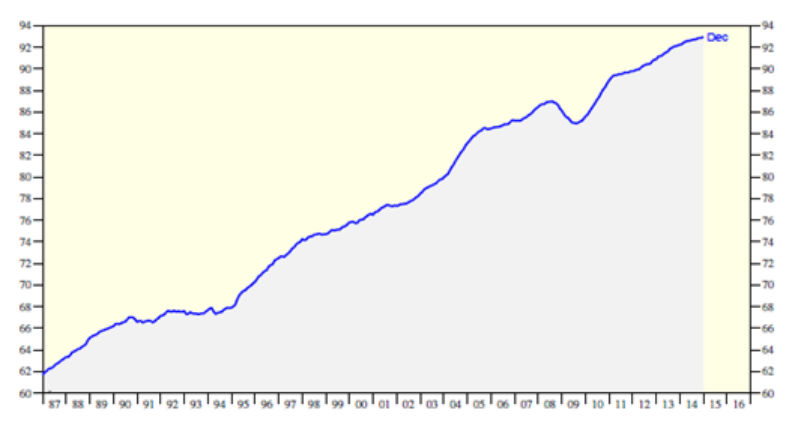
\includegraphics[width=\textwidth]{Marcteoric/Augmentdemandapetroli.png}
     	\caption{Demanda mundial de petroli, valor mig per any}
\end{figure}

En les grans ciutats ja comencen a aparèixer polítiques que prohibeixen l'entrada a vehicles que superen un cert grau de contaminació, ja que l'acumulació d'aquest pot pujar els nivells de contaminació de la ciutat per sobre del que regeix la llei. Els vehicles elèctrics no contaminen \newline pràcticament res, si no tenim en compte el seu procés de fabricació. Els vehicles híbrids funcionen amb electricitat fins que el motor ja ha de donar una certa potència, això ja suposa que el vehicle ha d'anar a una gran velocitat, fora de les velocitats màximes permeses en una zona urbanitzada. A més a més, el preu de la gasolina és molt elevat comparat amb el de l'electricitat. 

El preu d'un vehicle de combustió o un vehicle que funciona amb electricitat no és tant distant, no estem parlant que un cotxe elèctric pugui arribar a costar el doble d'un de gasolina, els preus es troben bastant parells, tot i que encara són més econòmics els de combustió. Es preveu que per al 2022 el cost total sense subsidi per als propietaris de bateria caurà per sota de la d'un vehicle de combustió. 

Per tots aquests motius i els preus assequibles dels vehicles elèctrics, el mercat dels VE es troba en augment. La previsió per als següents anys és que la demanda creixerà de forma exponencial. Al 2040 es preveu que els vehicles elèctrics seran un 35\% de les ventes mundials d'automòbils.

\begin{figure}[H]
		\centering
    	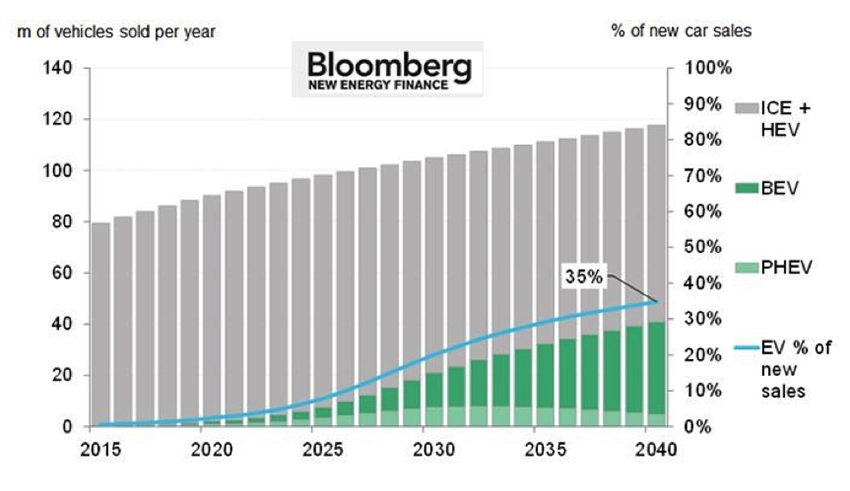
\includegraphics[width=\textwidth]{Marcteoric/ev-sales-distrib.png}
     	\caption{Previsió d'increment de la venda de vehicles elèctrics.}
\end{figure}

A la figura 2.2 es mostra de forma detallada la previsió de l'evolució del mercat dels vehicles. En primer lloc tindríem els ICE + HEV. Aquests vindrien a ser els vehicles que funcionen per combustió (dièsel/gasolina) i els híbrids que també fan servir la combustió. Es pot veure com són els que lideren encara el mercat, tot indicant que el petroli seguirà sent la font d'energia principal per als vehicles en general. 

En segon lloc tindríem els BEV(Battery Electric Vehicle) que són els vehicles que funcionen mitjançant bateries. Aquests assoliran un 30\% \newline d'increment l'any 2040. Per qüestions ecològiques que podrien succeir en el futur aquest valor pot decréixer considerablement si s'estableixen límits de contaminació molt baixos. Les subvencions de l'estat per als vehicles elèctrics també podria girar la balança i que agafessin en el futur un major pes.
 

En última instància hi ha els PHEV ( Plug-In Hybrid Electric Vechicle) que són els vehicles híbrids endollables a la corrent. Encara és incert el futur d'aquest tipus de vehicles i per això no hi ha gran confiança en aquests.

\section{Mercat dels vehicles elèctrics (no cotxes)}

Tot i que el món dels vehicles elèctrics està totalment centrat en els cotxes, també existeixen altres vehicles que fan servir l'electricitat com a font \newline d'energia. El controlador que es plantejarà en tot aquest projecte està pensat molt més per a aquest tipus de vehicles que no pas per a cotxes. Entre aquests vehicles podríem trobar el patinet elèctric, Hoverboard i la bicicleta elèctrica entre d'altres. No només això sinó que també el nostre controlador pot estar emprat per a vehicles dedicats a persones amb mobilitat reduïda com podria ser una cadira de rodes elèctrica o els típics "tricicles" que fa servir la gent gran. Per últim caldria posar els vehicles radiocontrol(RC), des de llanxes fins avions. 

Per a la majoria de vehicles esmentats no és precís aconseguir carnet de conduir o bé una llicència ni assegurança, però ve cal conèixer la normativa que regula l'ús d'aquests vehicles en llocs urbans. Cada municipi té els seus permisos i prohibicions. La normativa pot canviar depenent del pes o bé la velocitat màxima. Per això s'aconsella informar-se sobre la legislació del seu ajuntament. Sobretot a les grans ciutats és on la legislació és més estricta. Un exemple d'aquest podria ser la legislació actual de Barcelona sobre els patinets elèctrics. Els patinets elèctrics conformen els vehicles elèctrics de Tipus B.

\begin{figure}[H]
		\centering
    	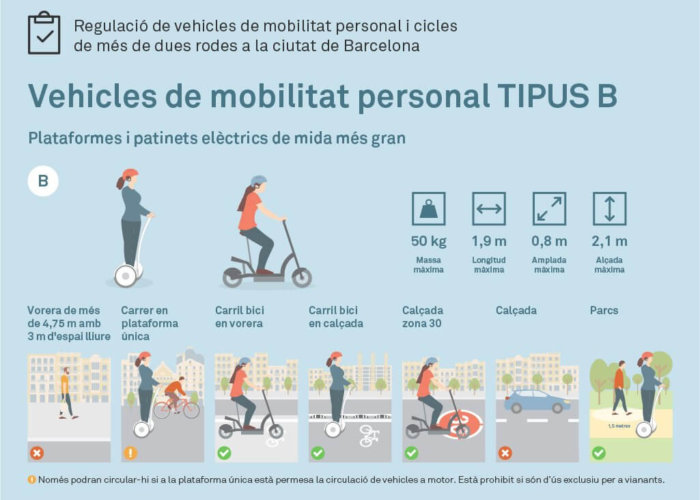
\includegraphics[width=12cm, height=7cm]{Marcteoric/normativaBCNpatinetselectrics.jpg}
    	\caption{Normativa de vehicles tipus B a Barcelona.}
\end{figure}

Si es parla de l'autonomia dels altres vehicles elèctrics no s'apropa ni de bon tros a l'autonomia d'un cotxe elèctric. Les autonomies d'aquests tipus de vehicles poden arribar als 40 minuts aproximadament, sent la bicicleta qui té una major autonomia. Depenent de la potència del motor, de la capacitat de la bateria i també com es condueixi aquest vehicle aquest temps pot variar. Un bon manteniment de la bateria també suposa una major durabilitat en l'autonomia. Ara es mostraran alguns vehicles elèctrics que són els que tenen un impacte més gran al mercat.

\subsection{Patinet elèctric}
El patinet elèctric és una opció alternativa de transport ecològic per circular a nivell econòmic sense gastar res en gasolina. Són sustentables, lleugers, pràctics i ràpids. Són útils tant per aquelles persones amb mobilitat reduïda, com per estudiants, treballadors i persones amb l'objectiu de desplaçar-se d'una forma senzilla d'un lloc a un altre en un curt període de temps, estalviant gasolina i transport públic.

L'enorme majoria dels patinets tenen un motor anomenat Brush (amb escombretes de llarga durada), de gama econòmica. Els patinets elèctrics dissenyat per la conducció del peu, on el seu diàmetre de roda és més gran, disposen d'un altre gènere de motor anomenat Brushless, que vindria a fer el mateix que el motor Brush, però sense escombretes. 

L'autonomia del patinet elèctric és la combinació de múltiples factors: La capacitat de la bateria (Volts i Amperes), la potència del motor (Watts), càrrega del patinet elèctric (massa pròpia), càrrega (massa conductor), inclinació del terreny i velocitat.
En línies generals, un patinet elèctric acostuma a tenir una autonomia d'entre 40 minuts en models de 800W a 55-60 minuts en els models de 1000-1500W.
\bigskip

\newpage 
\subsubsection{Xiaomi Mi Scooter}  
El Xiaomi Mi és el patinet elèctrics més venguts a la web d'Amazon. Està pensat per a una persona de fins a 75Kg. Té un abast de fins a 30Km amb una sola càrrega. Pot arribar a velocitats de fins a 35Km/h. El seu preu ronda els 380€. 
\begin{figure}[H]
		\centering
    	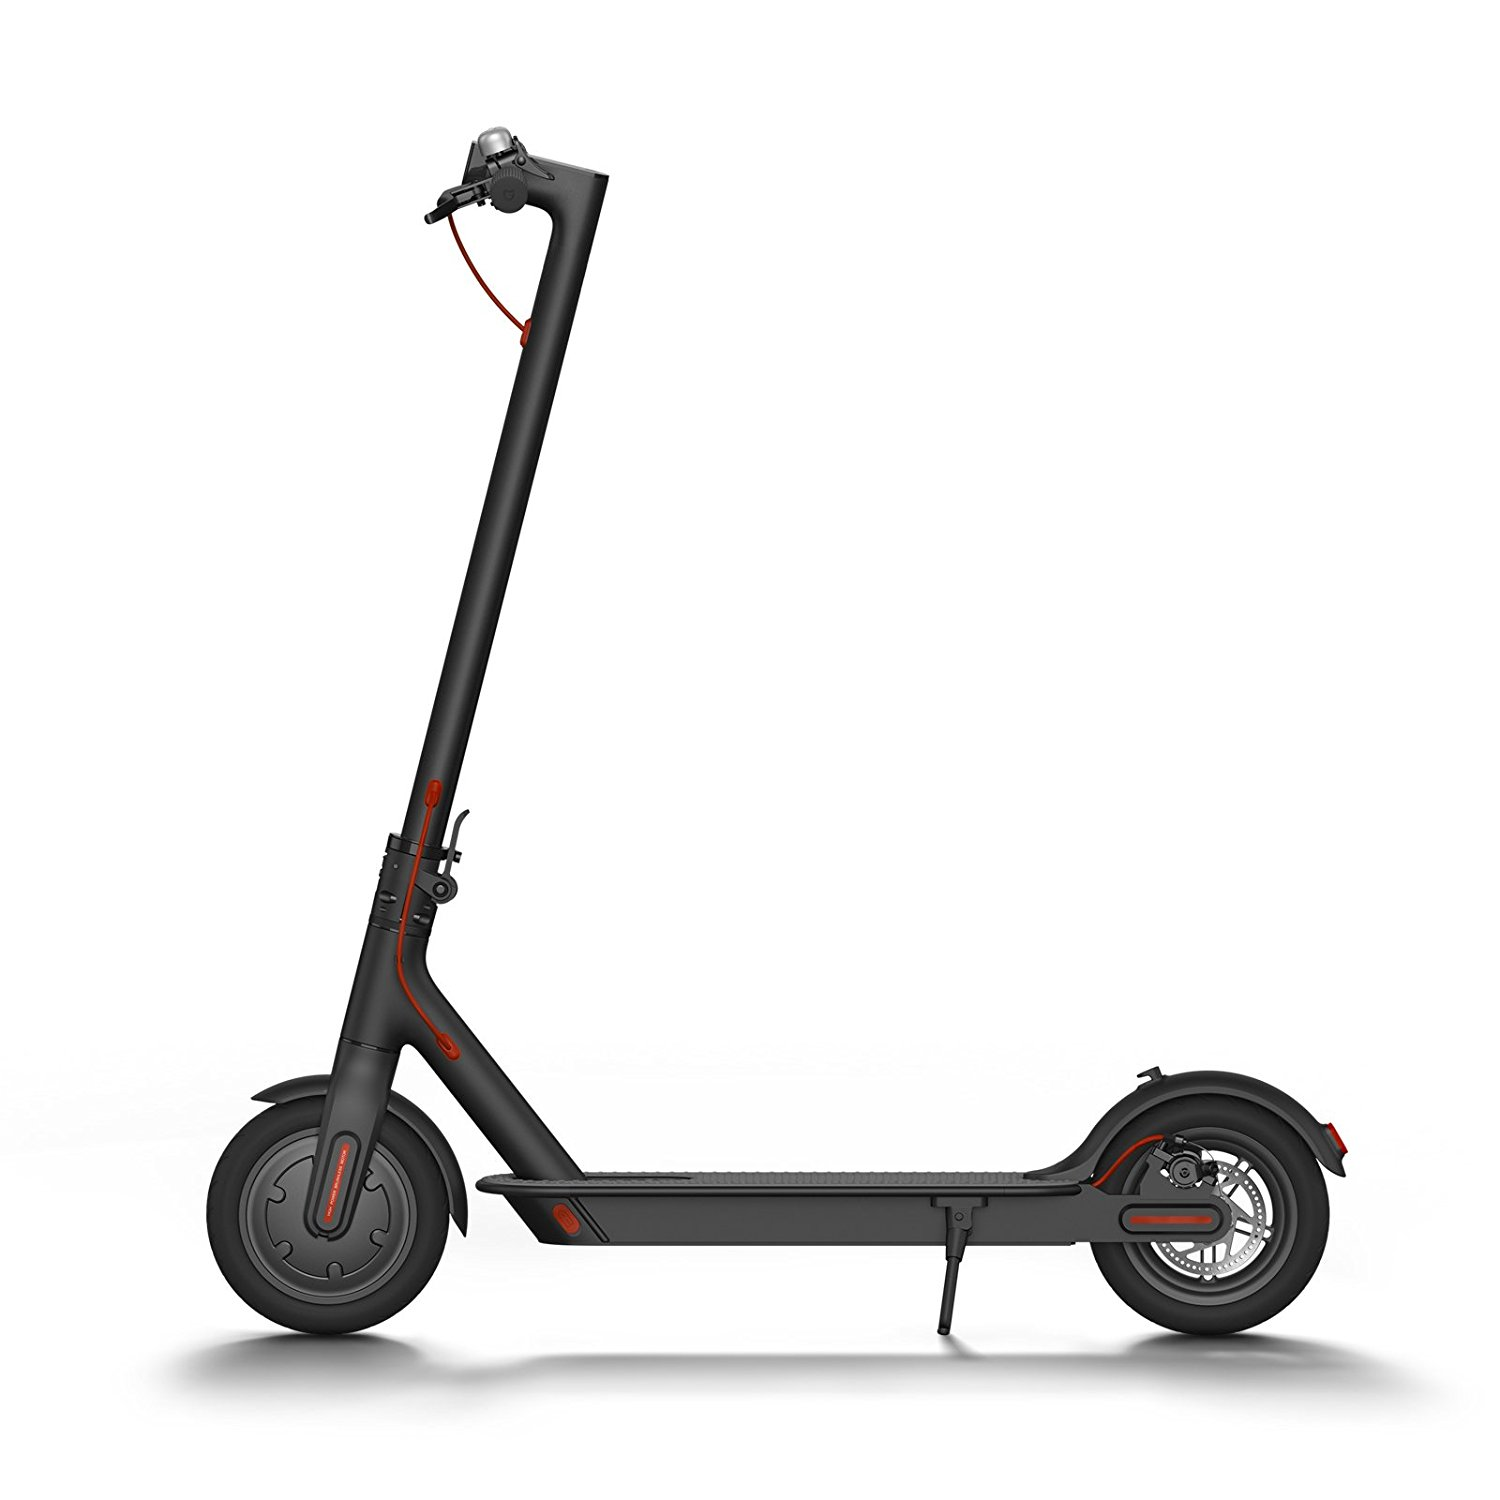
\includegraphics[width=10cm, height=10cm]{Marcteoric/patinetelectricxiamoi.jpg}
     	\caption{Xiaomi Mi Scooter.}
\end{figure}

\subsubsection{Homcom Patinet elèctric} 
El Homcom és un patinet plegable elèctric tipus Scooter, aquest model es trobaria a la gama baixa de patinets elèctrics. Està pensat per a una persona de fins a 50Kg. Té un abast d'entre 10-15Km amb una càrrega sencera. Pot arribar a una velocitat de fins a 12Km/h. El seu preu ronda els 100€.
\begin{figure}[H]
		\centering
    	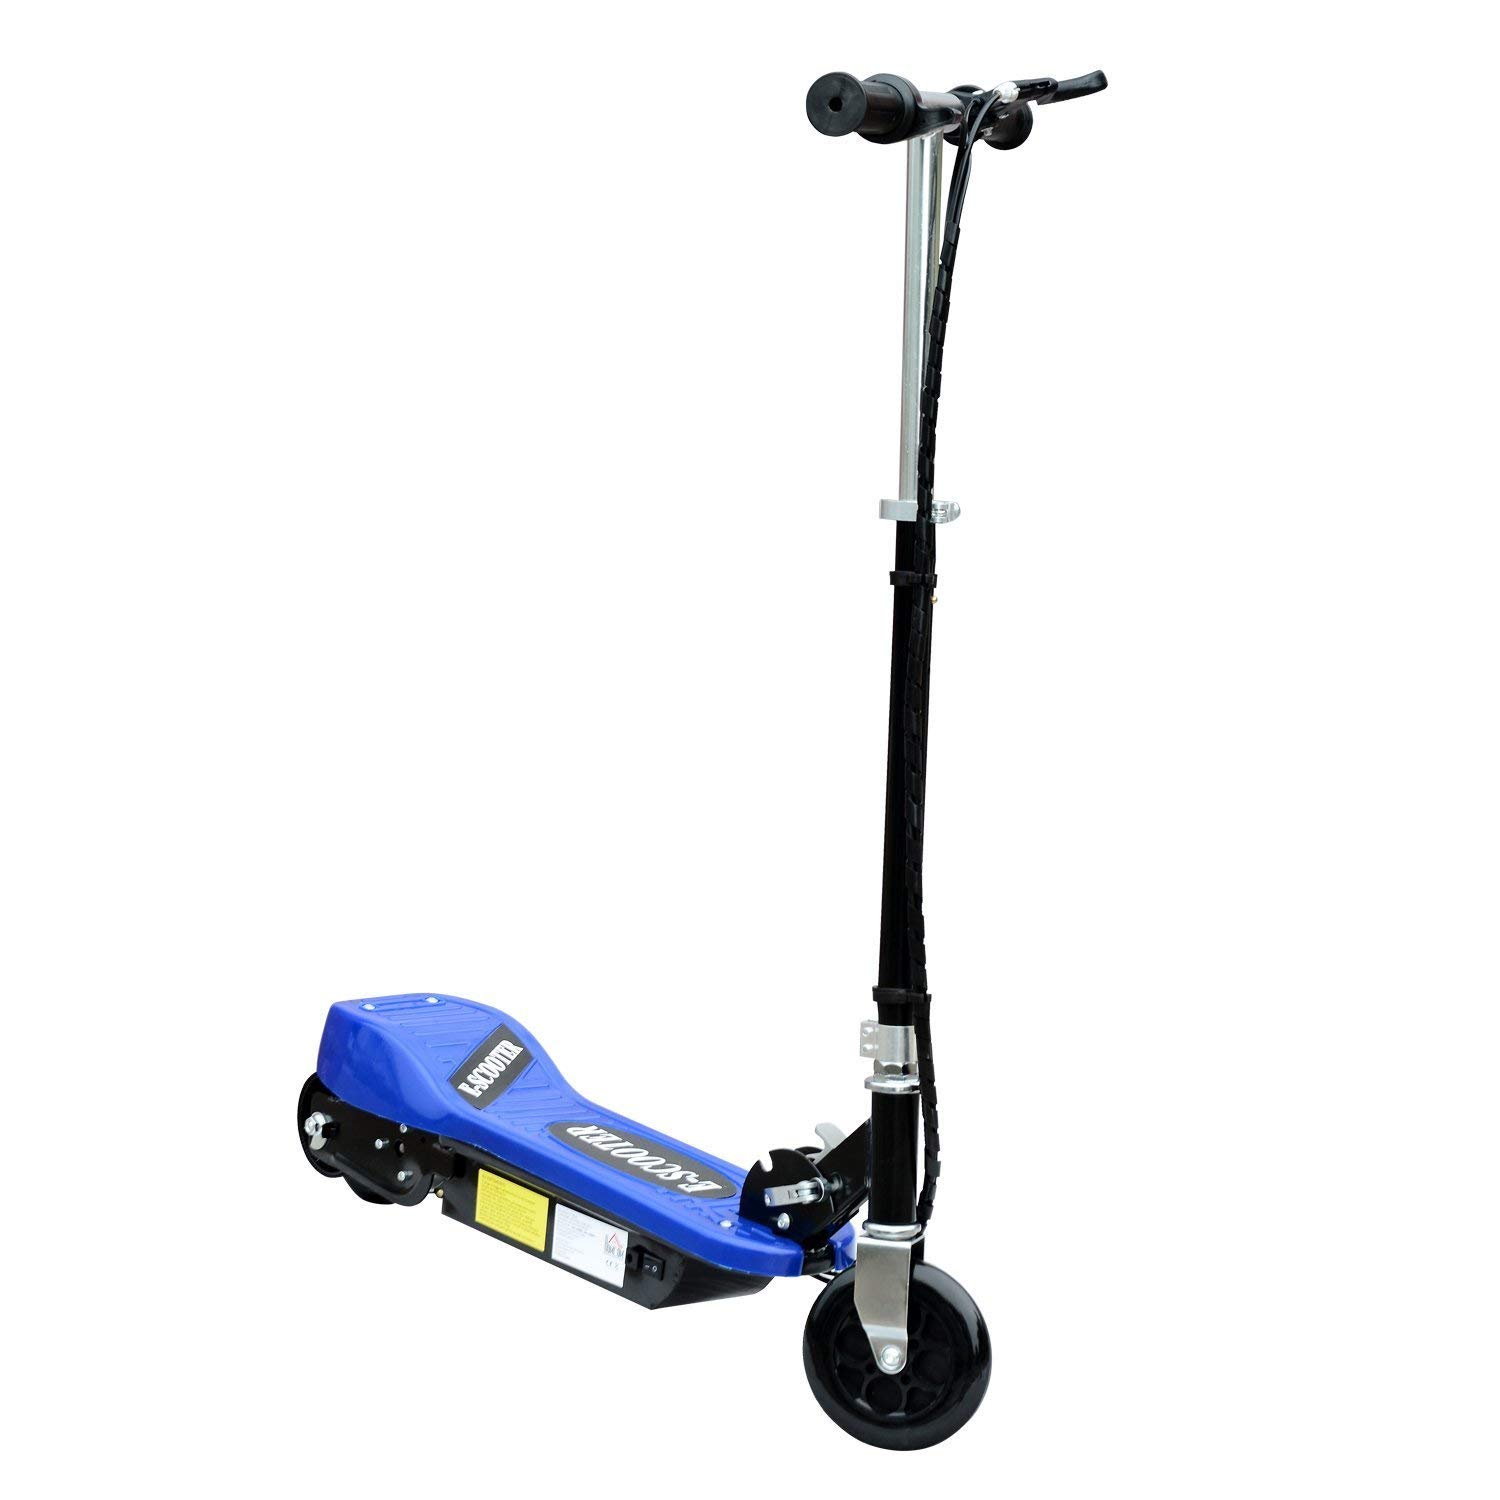
\includegraphics[width=8cm, height=8cm]{Marcteoric/Homcompatinetelectric.jpg}
     	\caption{Homcom patinet elèctric}
\end{figure}

\subsection{Hoverboard}
Aquests patinets han aparegut fa poc temps. Són únics en la forma en la que funcionen ja que s'autoequilibren, de tal forma que l'usuari pot accelerar i frenar tan sols movent el seu cos cap endavant o cap enrere. De la mateixa manera, girar és tan senzill com inclinar lleugerament el cos cap a un costat o l'altre. El funcionament d'aquest patinet es basa en el funcionament de diferents mecanismes. En primer lloc, les bateries es connecten a dos motors elèctrics independents en cada roda. Per altra banda, es troba el component més important per a mantenir l'equilibri, el giroscopi. Aquest detecta quan canvia d'orientació el patinet per a, d'aquesta forma, poder mantenir l'orientació adequada. 

El giroscopi funciona mitjançant un sensor magnètic que detecta la direcció de moviment i la velocitat rotacional de la roda. 
Tot el sistema es troba connectat a una unitat central de processament (CPU). El giroscopi mesura constantment l'orientació de la roda, i envia un senyal a la CPU per a que es processi e interpreti. D'aquesta forma, si el patinet s'inclina cap endavant s'envia l'ordre d'accelerar els motors per a compensar aquesta inclinació. Pel contrari, si s'inclina cap enrere es produirà l'efecte invers. Ara es mostraran dos exemples per veure com estan implantats aquests productes al mercat. \newline \bigskip

\subsubsection{Hooboard} 
El Hooboard és un Hoverboard de gama alta. Té una autonomia de fins a 15Km i una velocitat màxima de fins a 15Km/h. Està composat per dos motors de 400W i el seu preu ronda els 500€.
\begin{figure}[H]
		\centering
    	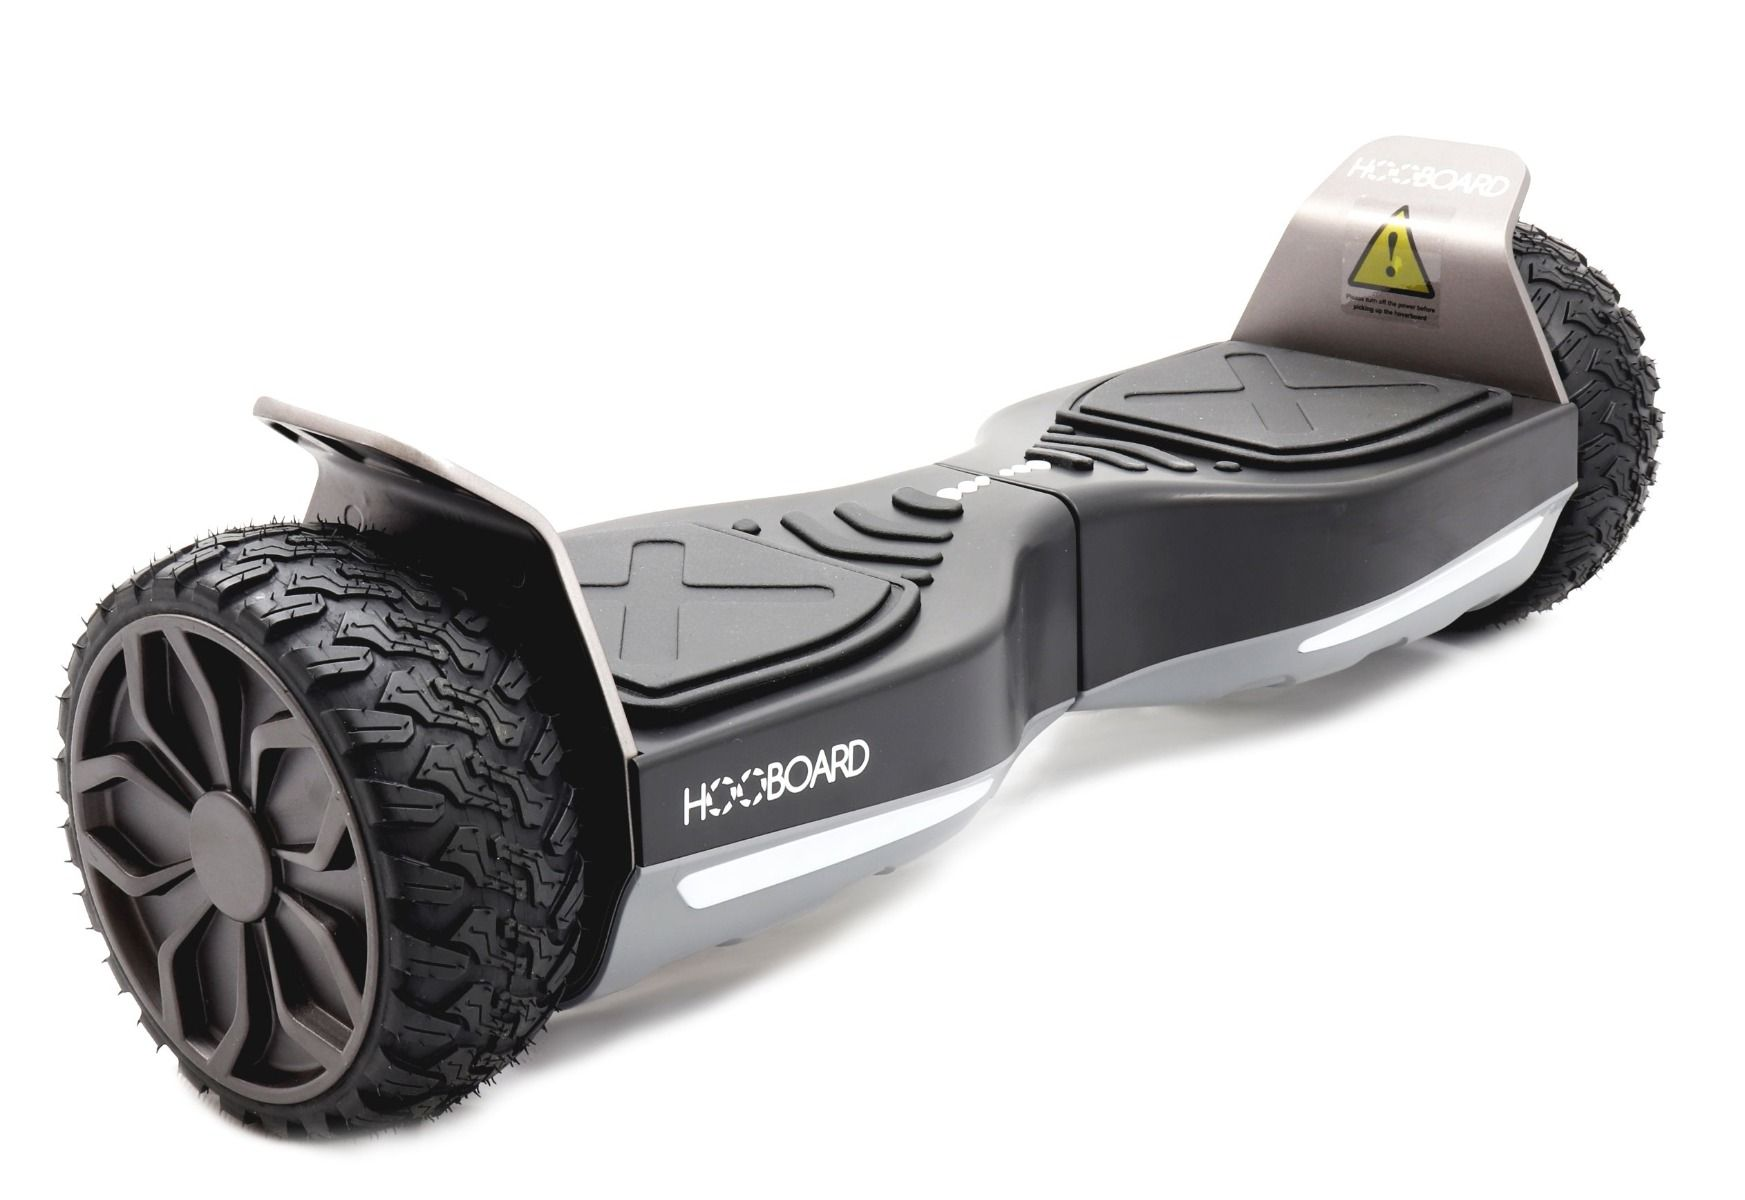
\includegraphics[width=7cm, height=5cm]{Marcteoric/hooboard.jpg}
     	\caption{Hooboard}
\end{figure}


\subsubsection{BEBK Hooverboard} 
El BEBK Hooverboard és un Hooverboard que funciona mitjançant motors elèctrics Brushless. Consta de dos motors de 350W. Pot arribar a velocitats de fins a 12Km/h i una autonomia de fins a 18Km. El seu preu ronda els 150€.
\begin{figure}[H]
		\centering
    	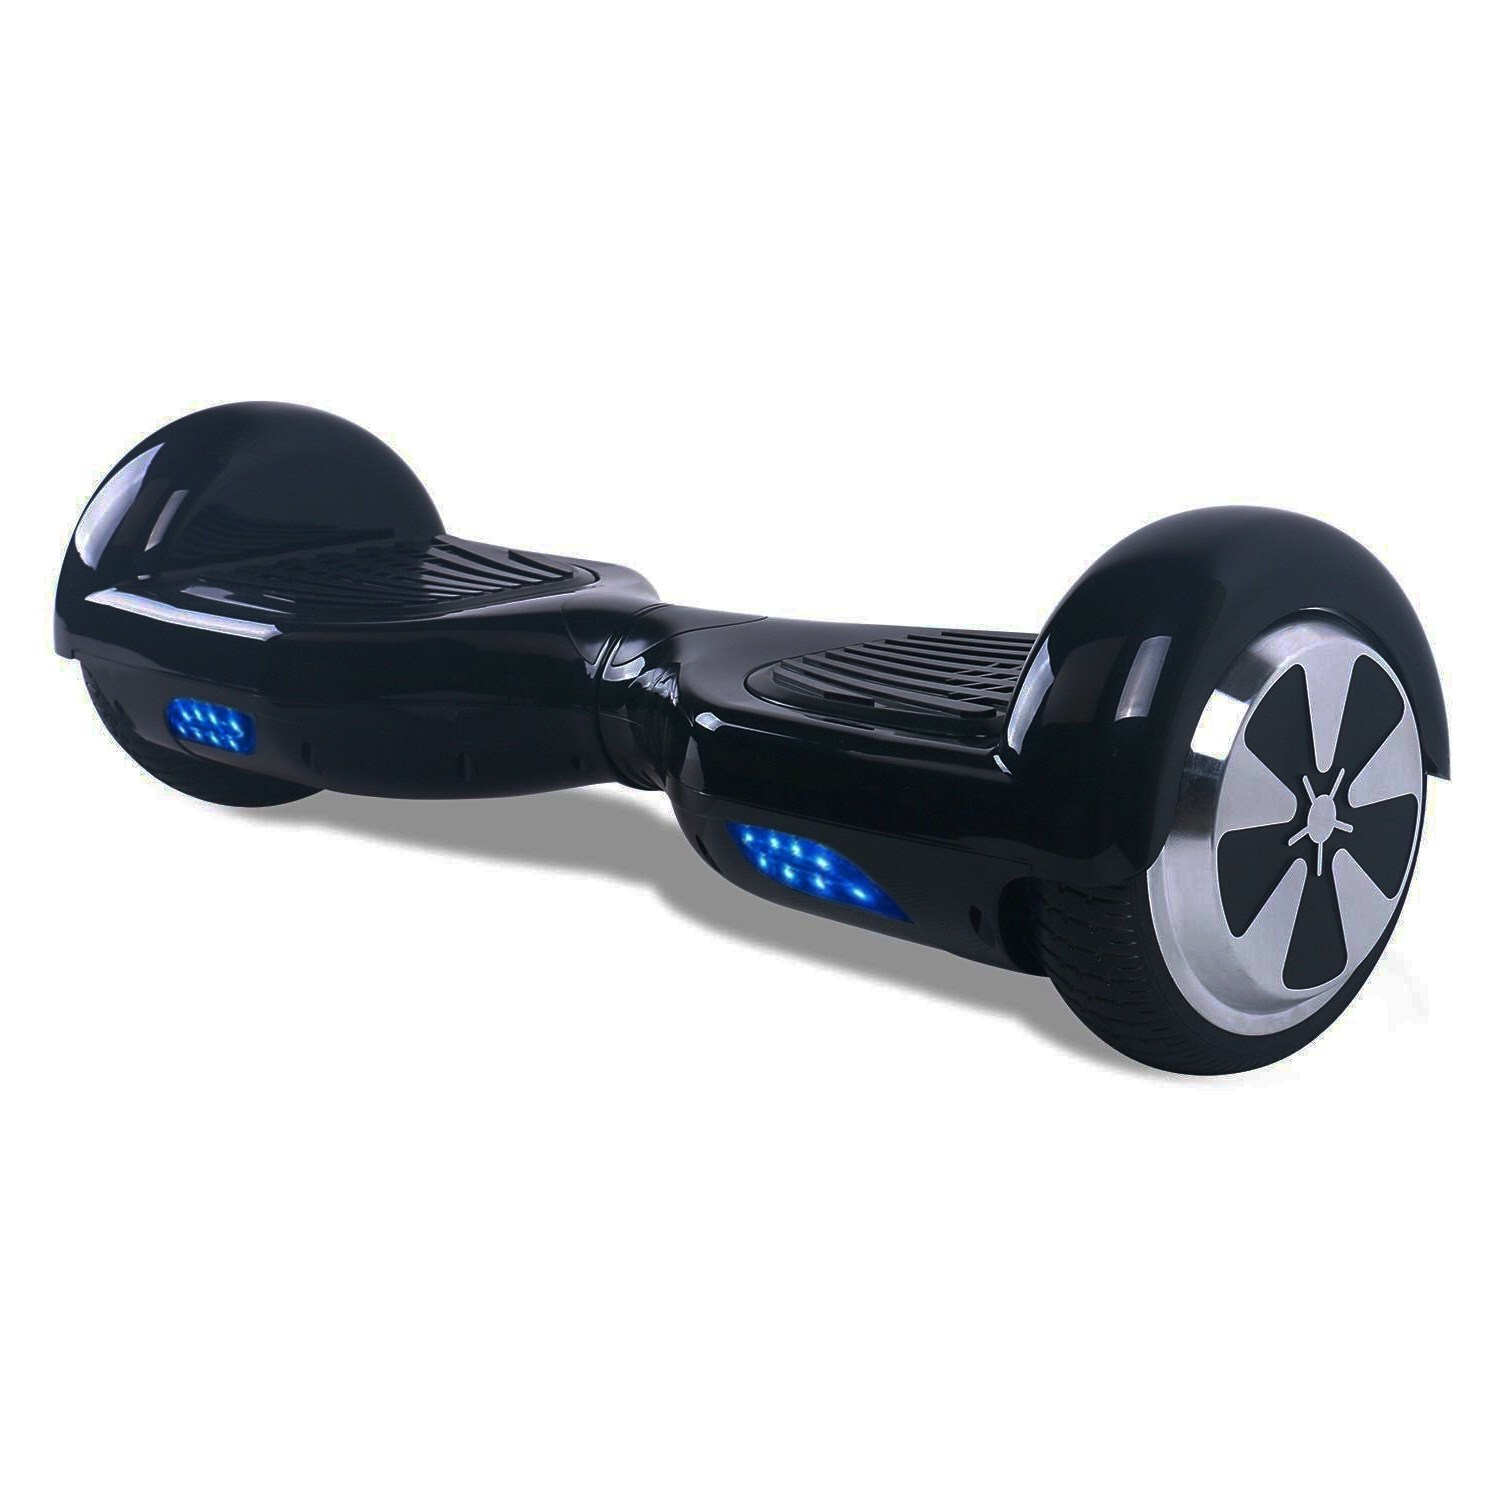
\includegraphics[width=7cm, height=7cm]{Marcteoric/bebkhooverboard.jpg}
     	\caption{BEBK Hooverboard}
\end{figure}

\subsection{Bicicleta elèctrica}
Al 2016 les ventes de bicicletes elèctriques van arribar, en tot el món, a uns 35 milions d'unitats. La millora de la tecnologia de les bateries d'ions de liti està donant com a conseqüència bicicletes elèctriques més lleugeres, més econòmiques i cada cop més similars a les bicicletes tradicionals.

Les altes tasses d'urbanització, la millora de la tecnologia de les bateries i els components de les bicicletes, les polítiques locals relacionades amb la contaminació, el desig creixent d'abandonar modes de transport motoritzats, el seu major rendiment i baix cost impulsen la indústria de la bicicleta elèctrica. Les bicicletes elèctriques es troben situades en una posició ideal per a ser les majors beneficiades d'aquesta tendència de canvi, pel seu baix cost en relació amb l'automòbil, per no requerir carnet pel seu maneig i per l'existència, cada cop en major mesura d'infraestructures especialment dedicades a elles. \newline \bigskip

             
\subsubsection{Extrbici XF800 Electric ATV } 
L'Extrbici XF800 Electric ATV és una bicicleta elèctrica que pot portar una càrrega de fins a 160Kg, pot arribar a 50Km/h amb una autonomia relativa de fins a 80Km. El seu preu rondaria els 1900€
\begin{figure}[H]
		\centering
    	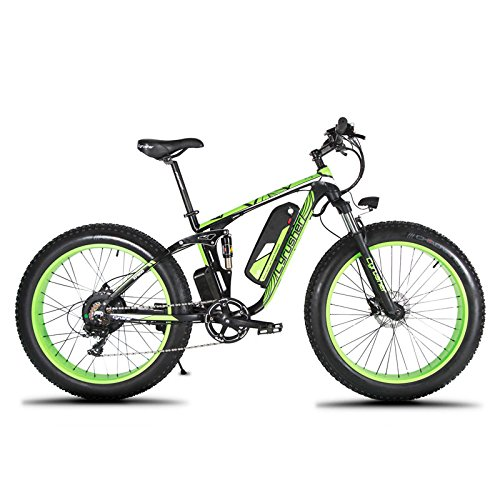
\includegraphics[width=8cm, height=8cm]{Marcteoric/extrbicixf800electricatv.jpg}
     	\caption{Extrbici XF800 Electric ATV}
\end{figure}
                      
\subsubsection{FOLLOW UP E05 }
El FOLLOW UP E05 és una bicicleta elèctrica que pot portar una càrrega de fins a 100Kg, pot arribar a 22Km/h amb una autonomia de fins a 30Km. Funciona amb motor Brushless de 250W i el seu preu ronda els 400€.
\begin{figure}[H]
		\centering
    	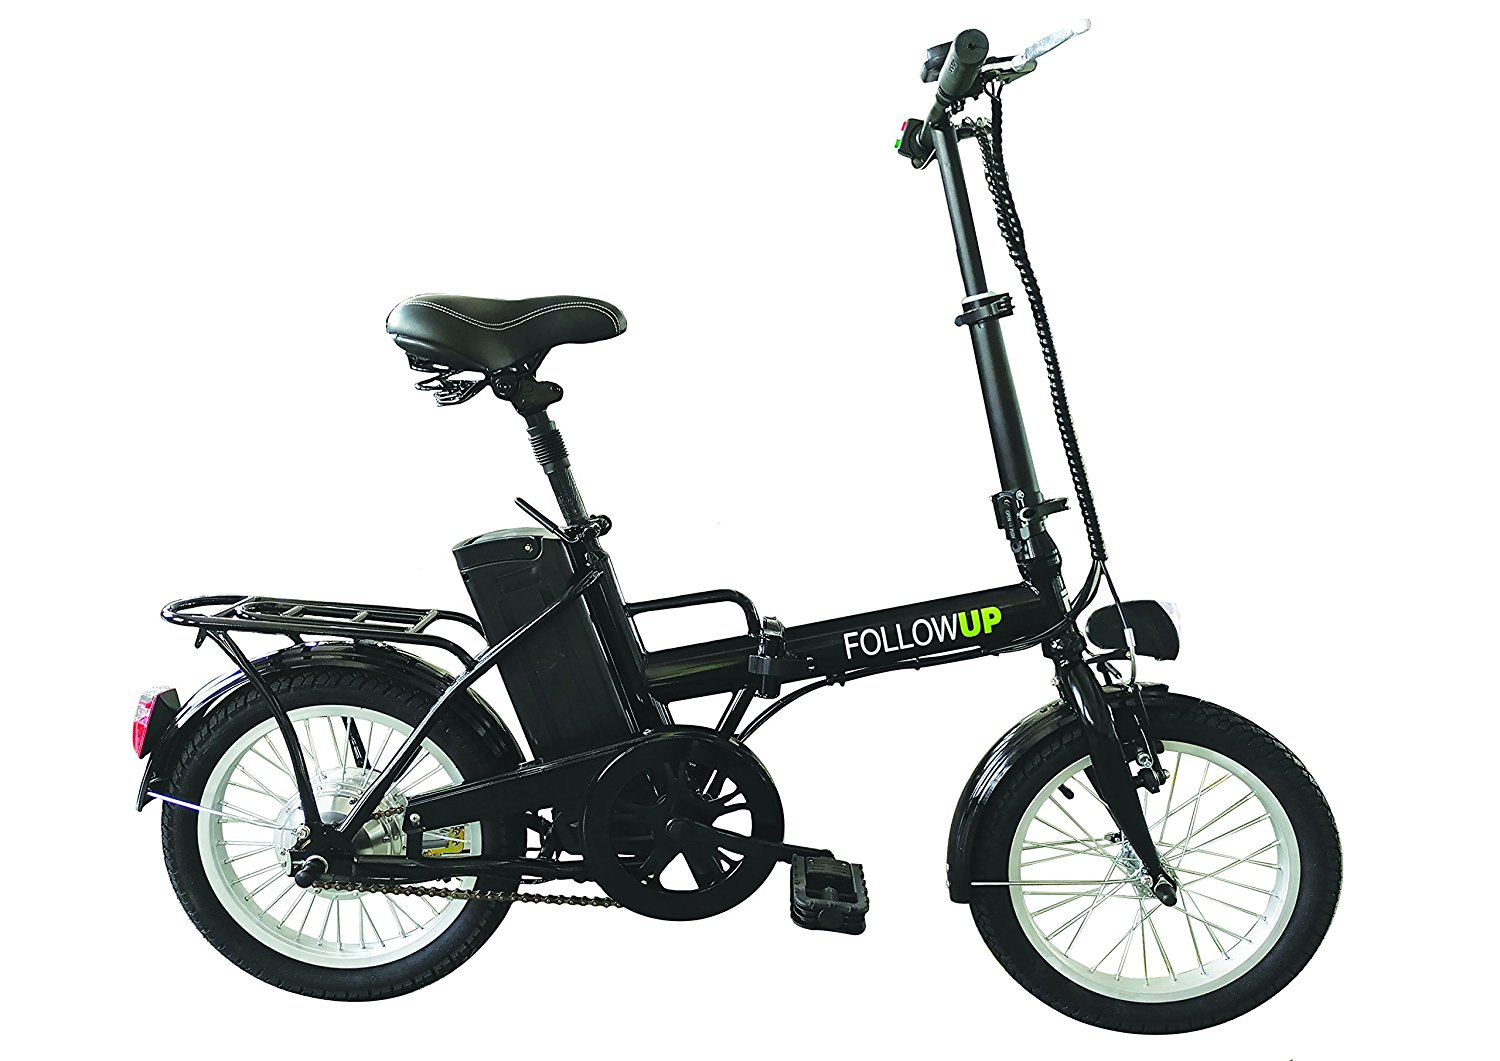
\includegraphics[width=10cm, height=7cm]{Marcteoric/followupe05.jpg}
     	\caption{FOLLOW UP E05}
\end{figure}

\section {Mercat de les bateries emprades per als VE}
Les bateries d'ions de liti ja formen part de la vida quotidiana i estan incloses en telèfons mòbils, tauletes i raspalls de dents elèctrics, entre d'altres aplicacions. En els últims anys s'han produït diferents avenços tecnològics en aquest tipus de bateries per a poder ser emprades en els vehicles elèctrics. Encara que l'adopció dels vehicles elèctrics no estigui sent tan positiva com s'esperava, les bateries ja suposen un component cada cop més rellevant dins de la indústria automobilística. Donat que les bateries són una part significativa dels costos d'un vehicle elèctric, existeixen considerables incentius per augmentar l'eficiència dels seus processos de producció, reduir els seus costos i millorar el seu rendiment. El sistema elèctric es beneficiarà del desenvolupament d'aquestes bateries, al construir una solució per emmagatzemament de l'energia generada per les tecnologies renovables intermitents, que permetran reforçar la seva seguretat de subministrament.

Respecte als reptes que té aquesta tecnologia a superar, cal destacar la falta d'una única tecnologia d'emmagatzemament que sigui capaç de cobrir totes les necessitats del mercat. Això provocarà que el sistema pugui contemplar la incorporació de diferents tipus de bateries. 

Addicionalment, a l'igual que qualsevol altre component del sistema elèc- \newline tric, els sistemes de gestió de bateries hauran de lidiar amb els possibles atacs tecnològics que puguin sofrir. En definitiva, el desenvolupament dels vehicles elèctrics permetrà avançar en les tecnologies de bateries \newline d'emmagatzemament. Les bateries hauran de considerar-se com a part de l'estratègia de les energies renovables, contribuint a arribar a un sistema energètic més eficient.

\subsection{Previsió de mercat per al futur de les bateries}

Com ja s'ha comentat prèviament, les bateries jugaran un paper molt important dintre dels vehicles elèctrics. Això vol dir que ja s'implementen estratègies per tal d'optimitzar el màxim els costos i rendiment d'aquestes. A la dècada del 2030 podríem estar parlant que el preu de baixada respecte el 2010, que és quan van començar a aparèixer de forma global les bateries d'ió-liti, estaria suposant aproximadament una reducció de cost de fins al 75\%. No només es reduiran els preus de les bateries, sinó que la compra \newline d'aquestes bateries augmentarà considerablement en els últims anys arribant a valors que superin els catorze mil milions de dòlars l'any 2026.
\begin{figure}[H]
		\centering
    	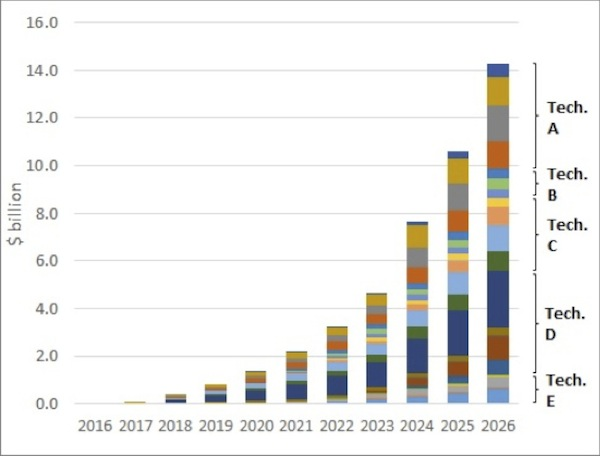
\includegraphics[width=13cm, height=8cm]{Marcteoric/ventabateries2026.jpg}
     	\caption{Previsió de ventes de bateries en funció del tipus de vehicle.} 
\end{figure}

\subsection{L'hora de l'economia del liti}
Les bateries de liti estan totalment consolidades a la vida quotidiana. Són necessàries per alimentar des de petits dispositius fins a sofisticats vehicles elèctrics. La previsió és que el seu consum augmenti en els pròxims anys, especialment fomentat per l'auge de l'Internet de les Coses i altres aplicacions tecnològiques.

Degut a la predicció del decreixement del cost d'aquest tipus de bateries s'està impulsant de forma massiva aquest mercat. Aquesta caiguda de preus és probable que provingui d'un augment de la demanda degut a la propagació dels cotxes elèctrics, que està permetent als fabricants augmentar la producció. 
\begin{figure}[H]
		\centering
    	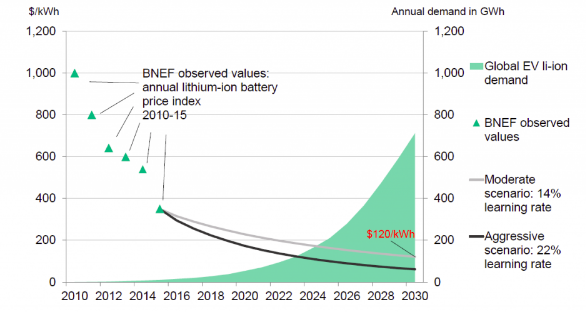
\includegraphics[width=13cm, height=8cm]{Marcteoric/mercatbaterialitioion.png}
     	\caption{Previsió del mercat de les bateries d'ions del liti.} 
\end{figure}

\section{Recerca de gestors de bateries al mercat}
Al mercat actual no existeixen controladors de vehicles totals, és a dir, un controlador que s'encarregui de tot el procés de control de la bateria fins al control del motor. Al mercat queda diferenciat en aquests dos grans blocs que normalment són compatibles entre ells. És per això que cal buscar per separat els gestors de bateries i els drivers del motor. Com el meu projecte va enfocat als BMS exposaré un exemple per després contrastar-ho amb la nostra idea de prototip. El BMS que es mostrarà a continuació es l'Orion BMS.

\subsection{Orion BMS}
Si es busca un BMS de confiança per a gestionar bateries de liti l'Orion BMS és una opció a tenir molt en compte. És un molt bon gestor de bateries altament valorat en el mercat. La seva fiabilitat i totes les seves característiques fan que sigui un BMS de molt alta gama. Compta amb una interfície per a que l'usuari el pugui configurar. Pot controlar des de 24 fins a 180 cel·les i el seu preu es troba entre els 1,000\$ i els 2,300\$.

Les seves característiques elèctriques serien les següents:

\begin{figure}[H]
		\centering
    	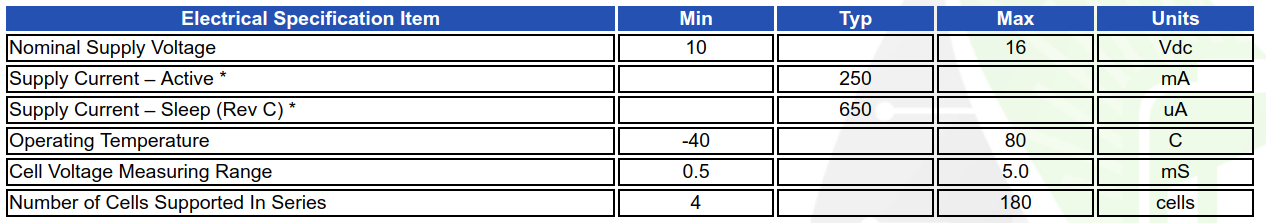
\includegraphics[width=\textwidth]{Marcteoric/electricalspecsorionbms.png}
     	\caption{Característiques elèctriques de l'OrionBMS.}
\end{figure}

Les seves especificacions generals serien les següents:

\begin{figure}[H]
		\centering
    	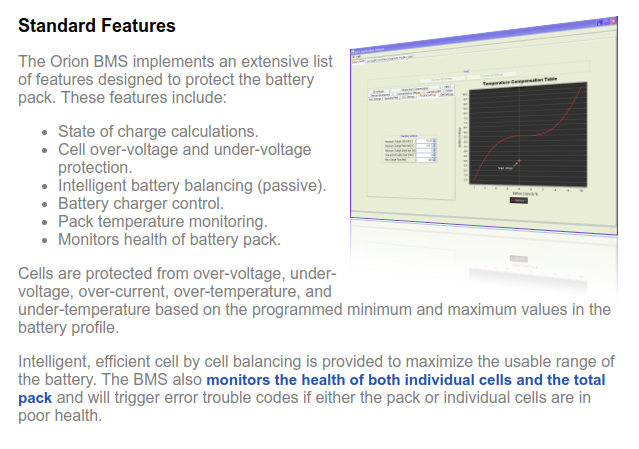
\includegraphics[width=12cm,height=5.5cm]{Marcteoric/stdftsorionbms.png}
     	\caption{Especificacions generals de l'OrionBMS.}
\end{figure}

La seva interfície per a l'usuari és la següent:

\begin{figure}[H]
		\centering
    	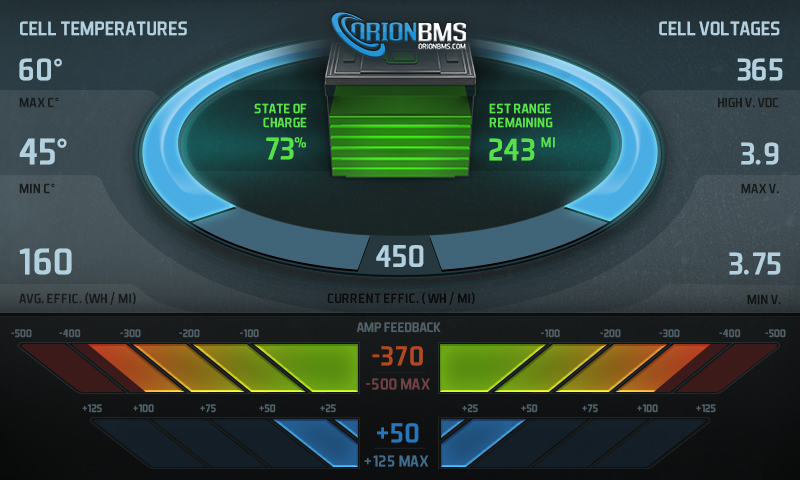
\includegraphics[width=\textwidth,height=7cm]{Marcteoric/orionbmsinterface.jpg}
     	\caption{Interfície de l'OrionBMS per a l'usuari.}
\end{figure}

No es vol entrar molt en detall ja que aquests fabricants tenen protocols privatius els quals no indiquen com realitzen per exemple l'estimació del SOC, un dels principals paràmetres a tenir en compte en un BMS. Sent tot privat és molt complicat contrastar-ho a nivell tècnic.

Els comentaris respecte aquest BMS són molt positius, però tenim encara la qüestió de que són encara molt cars. Si el nostre BMS l'aconseguim realitzar podríem estar competint a nivell de preu de venta, pensant en el nostre projecte com a producte. Si només el contemplem com un projecte per a nosaltres per aconseguir gestionar correctament una bateria, el preu disminuiria altament, per tant a nivell de preu estem en una molt bona posició.

\section{Recerca de projectes de codi obert de BMS}

Existeixen molts projectes de codi obert basats en gestors de bateries. Uns només mostren el software i altres només donen el hardware. És molt complicat doncs implementar un BMS en la seva totalitat en projectes de petita escala. No obstant, hi ha un projecte que s'ha diferenciat de la resta per ser un dels més complexes. Aquest projecte s'anomena Fox BMS.

\subsection{Fox BMS}
Avui en dia existeix un dels projectes més grans d'un disseny de BMS de codi lliure anomenat Fox BMS. És gratuït, obert i flexible per a entorns de recerca i desenvolupament per al disseny de BMS. La part més increïble és que és la primera empresa que dóna en la seva totalitat tant la part de hardware com la part de software. El fet d'oferir tot el projecte a la comunitat ha fet que la pròpia comunitat hagi desenvolupat encara més aquest projecte. Aquesta comunitat no està només composada per petites comunitats de gent, o individus, sinó que també grans empreses han participat en aquest projecte. El fet de que les grans empreses hagin participat en aquest projecte ha sigut el punt clau per a que aquest projecte sigui mundialment conegut en l'entorn de les bateries.

Els creadors d'aquest BMS han desenvolupat fins i tot un vehicle elèctric, obert al mercat, que funciona amb aquest gestor de bateries. L'estructura complerta d'aquest projecte es mostra a la següent figura:

\begin{figure}[H]
		\centering
   	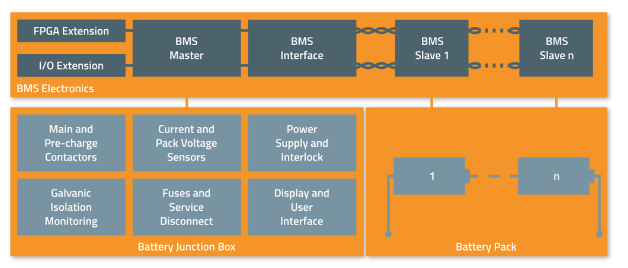
\includegraphics[width=\textwidth, height=6cm]{Marcteoric/estructurafoxbms.png}
     	\caption{Arquitectura del FOX BMS.} 
\end{figure}

El FOX BMS és un BMS modular de desenvolupament, amb l'objectiu de controlar les bateries per a l'automoció, l'aviació, l'espai, vaixells, trens, bateries industrials i per a energies renovables. És un projecte que està sempre en desenvolupament. Totes les característiques que dóna aquest BMS queden reflectides en la següent figura:

\begin{figure}[H]
		\centering
   	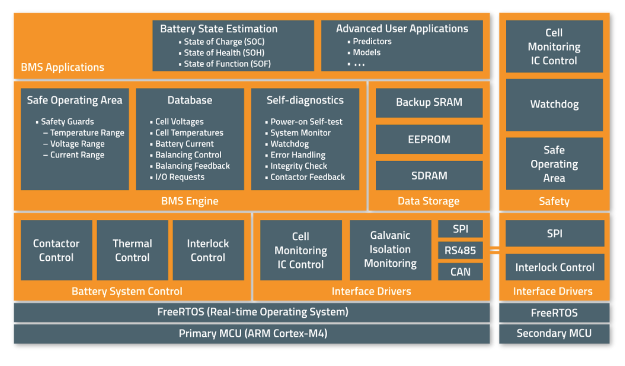
\includegraphics[width=\textwidth, height=6cm]{Marcteoric/aplicacionesfoxbms.png}
     	\caption{Característiques del FOX BMS.} 
\end{figure}

Les funcions principals d'aquest BMS són compartides amb la majoria de BMS del mercat. Bàsicament és poder fer l'estimació tant del SOC com del SOH, que és principalment el control constant de les cel·les per assegurar que funcionen correctament. També controlen la temperatura de les cel·les. No obstant, aquest projecte compta amb moltes més característiques que fan que sigui un dels BMS més potents del mercat. \newline D'aquestes característiques destaquen tant el monitoreig constant de les cel·les com algorismes que prediuen aspectes futurs que poden succeir a les cel·les. D'aquesta manera el sistema queda molt més robust ja que prediu els possibles errors amb un cert marge de temps, suficient com per evitar problemes. 
\bigskip
\begin{figure}[H]
		\centering
   	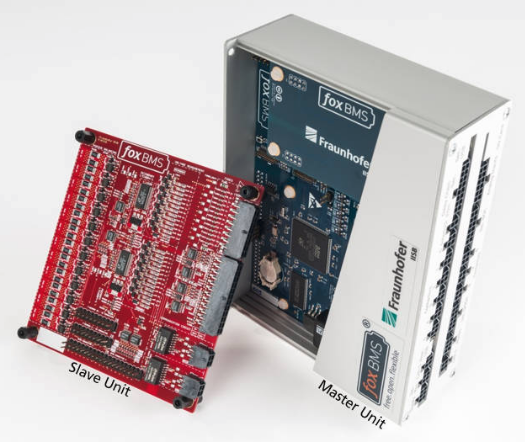
\includegraphics[width=8cm, height=7cm]{Marcteoric/foxbmsimatge.png}
     	\caption{Model de venta del FOX BMS.} 
\end{figure}

Aquest projecte és massa complex per a una persona que comença a \newline conèixer el món dels gestors de bateries. És per això que només s'han esmentat els seus aspectes principals. 

\section{Marc del projecte}
Per desenvolupar un BMS cal conèixer en primer lloc quines bateries existeixen i quines són les seves característiques principals. Això quedarà explicat en el següent capítol del projecte, en l'apartat de bateries. Un cop vistes les diferents bateries es procedirà a fer l'elecció d'un tipus d'aquestes, el qual servirà de base per a la implementació del BMS. És a dir, que el BMS es realitzarà en funció del tipus de bateria que s'esculli. Un cop escollida la bateria es tornarà a indagar sobre els diferents conceptes amb els quals treballa un BMS i finalment es procedirà en la implementació teòrica d'un BMS. Aquest integrat quedarà representat de forma esquemàtica amb \newline l'electrònica mínima que requereix per a veure la implementació d'aquest. 

\chapter{Bateries}
\label{chap:Bateries}

Avui en dia ens trobem rodejats de bateries: en els telèfons mòbils, en els portàtils, en els automòbils, etc. Hi ha de molts tipus: d'àcid-plom, de níquel i hidrur metàl·lic, de liti... En un futur seran potser l'element més important per a la tecnologia, ja que es convertiran en la font d'energia més emprada per a qualsevol aparell sense fil. 

Per a fer un gestor de bateries, és essencial conèixer el camp de les bateries, de tots els conceptes que cal tenir en compte, tant avantatges com desavantatges i així poder valorar d'una forma més crítica per a la realització d'un prototip, escollir primerament quines serien les bateries que es farien servir, per tal de poder fer un BMS més adaptat a les necessitats d'aquesta. 

\section{Concepte de bateria}

Una bateria és un dispositiu que permet produir electrons a partir d’una reacció química, el que es coneix com reacció electroquímica. Si fem una ullada a qualsevol bateria podem observar com aquesta posseeix dos terminals o bornes. Un d’ells sol estar marcat amb un signe positiu “+” mentre que l’altre posseeix un signe negatiu “-”. Al cablejar aquests dos terminals, els electrons flueixen, tan ràpid com poden, des del terminal negatiu cap al terminal positiu. Normalment es sòl col·locar algun tipus de càrrega en aquesta connexió, com una llum o un motor.

A l’interior de la bateria, una reacció química produeix aquests electrons a una tassa determinada (resistència interna). Per a que la reacció tingui lloc, els electrons han de poder desplaçar-se des del pol negatiu al positiu. Aquesta és la raó per la qual podem teòricament deixar una bateria desconnectada i no perdre aquesta energia. Mentre que si deixem el circuit connectat, el flux d’electrons farà que la bateria es descarregui.

Les bateries es componen d’una o varies cel·les. De fet el terme bateria fa al·lusió a que les cel·les es col·loquen una darrera de l’altre en sèrie per augmentar la capacitat i la tensió de l’acumulador elèctric. Existeix una certa similitud amb el terme pila que es va començar a fer servir perquè les cel·les formen una pila ja que es col·loquen unes damunt de les altres. Però que es una cel·la? Doncs és una espècie de caixa tancada on en el seu interior hi ha dos elèctrodes submergits en un electròlit. Els elèctrodes a la vegada es comuniquen amb l’exterior mitjançant bornes que és on la bateria es connecta al sistema elèctric.

Dintre de les cel·les, entre cada un dels elèctrodes i electròlit, es produeixen unes reaccions químiques reversibles que són las que cedeixen o absorbei- \newline xen electrons. Això genera una tensió elèctrica entre els elèctrodes i per tant entre les dues bornes de la cel·la.                    

\section{Funcionament i usos}
Els processos químics que s'efectuen dins una bateria es coneixen com reaccions redox o de reducció-oxidació. Així dit d'una forma col·loquial en la reducció, els reactius es combinen per a formar altres substàncies químiques més reduïdes i durant aquest procés absorbeixen electrons. \newline L’oxidació és el procés invers. Les substàncies reduïdes es combinen per a formar altres compostos més oxidants i durant el procés s’alliberen \newline càrregues negatives(electrons). Quan la bateria s’està descarregant en \newline l’elèctrode negatiu es produeix una reacció d’oxidació i en el positiu de reducció. Quan la bateria està carregant succeeix l’efecte contrari, l’oxidació es produeix en l'elèctrode positiu i la reducció en el negatiu.

Aquestes reaccions redox no es poden donar de forma indefinida. Després de centenars o milers de cicles de càrrega-descàrrega, el material dels elèctrodes es va debilitant i espatllant de mica a mica a mida que es fan servir fins a espatllar-se completament. Aquesta degradació dels elèctrodes depèn del tipus de tecnologia i de les condicions d’ús: temperatura de funcionament, profunditat de descàrrega...

Actualment, la investigació de millors bateries es centra en la tecnologia d'ions de liti ja que és l’element químic que més tensió genera al produir-se la reacció redox; 3.7V. On s’està treballant per millorar la capacitat de les actuals bateries és en els elèctrodes. Quan major sigui la superfície de contacte dels elèctrodes amb l'electròlit, les reaccions químiques es podran produir en major volum i per tant augmentar la seva capacitat.                 

\section{Mètodes de càrrega de bateries}
L'objectiu d'un carregador és carregar la bateria. Però hi ha moltes altres característiques que poden millorar el funcionament d'un carregador i concedir protecció a la bateria que s'estigui carregant. Aquestes característiques integrades són les que protegeixen la bateria d'un mal funcionament.

Els carregadors de bateries ofereixen característiques o algorismes de \newline càrrega especials els quals tenen com a objectiu millorar el funcionament d'una bateria, reduint el temps de càrrega i augmentant la seva vida útil.

Els conceptes que s'han de tindre en compte a l'hora de dissenyar un carregador de bateria o el algorisme que el controli són:

\begin{itemize}
    \item L'adaptació del voltatge i la intensitat en funció de la temperatura redueix l'evaporació de l'electròlit i els danys en els elèctrodes.
    \item Un alt corrent acabarà reduint la vida útil de la bateria.
    \item La càrrega a polsos pot ajudar a una càrrega complerta.
    \item Una correcta limitació del voltatge redueix l'evaporació de l'electròlit prevenint l'efecte \textit{dry-out}\footnote{Assecament de l'electròlit d'una bateria}.
\end{itemize}

Tradicionalment els carregadors de bateries més simples no regulaven bé els límits de tensió i corrent, únicament es dedicaven a injectar-la. Amb els avenços del sector s'han desenvolupat carregadors de major qualitat capaços de reduir els temps de càrrega, de millorar la protecció contra sobre voltatges i augmentar la vida útil. Tots aquests motius fan que sigui molt més viable treballar amb bateries a nivell econòmic i de seguretat. S'han desenvolupat diferents models els quals seran exposats de forma teòrica a continuació:

\subsubsection{Càrrega a corrent i tensió constants}
És un mètode simple de càrrega que dóna bons resultats sempre i quan els límits de corrent i tensió estiguin ben definits. La càrrega de la bateria comença sent a corrent constant fins que arriba a una determinada tensió en els pols de la bateria. A partir d'aquest moment la càrrega continua però ara a tensió constant i variant la intensitat la qual va reduint-se fins a arribar a un valor en el qual es considera que la bateria està totalment carregada. També es pot controlar si la bateria està completament carregada en funció del temps de càrrega, encara que aquest mètode no és el més aconsellable. 

\subsubsection{Càrrega per goteig}
Aquest mètode és molt semblant a l'anterior, amb la diferència de que aquest permet carregar la bateria fins al 100\% de la seva capacitat. És un mètode efectiu però lent. Aquest tipus de càrrega sol estar associat a bateries d'àcid-plom les quals tenen un corrent baix de gasificació. La idea d'aquest mètode consisteix en subministrar en el procés final de càrrega un corrent molt petit que a condicions de temperatura i tensió pot arribar a ser inferior a una trentena part de la intensitat nominal de la bateria. Aquest mètode de càrrega és també conegut com càrrega de manteniment i s'utilitza per a compensar l'auto-descàrrega de les bateries. 

\subsubsection{Càrrega mitjançant polsos}
Aquest mètode de càrrega consisteix en enviar corrent a la bateria durant períodes molt curts de diversos mil·lisegons en comptes d'estar permanentment amb tensió de càrrega. La duració del pols és la que determina el nivell final de corrent de càrrega subministrada. L'utilització d'un carregador de bateries per polsos aconsegueix mantenir la joventut de la bateria i fer-la viure molt més temps.

\section{Tipus de bateries}
Depenent del material amb el qual estiguin construïts els elèctrodes i de les substancies que formen l’electròlit existeixen diferents tipus de bateries. 

\subsection{Bateries d'un sol ús o recarregables}
Abans de parlar dels tipus de bateries en funció del seu material és important separar els dos grans grups del món de les bateries. Aquests dos grans grups són les bateries recarregables i les d'un sol ús, també conegudes com primàries i secundàries. Les bateries o acumuladors d'un sol ús, com el seu nom indica són d’un únic ús, després es tornen inservibles ja que la reacció química interior s’ha esgotat. Les més comunes d’aquest tipus serien les de zinc carboni o les alcalines, les primeres de menor rendiment que les segones. Les utilitzem en tot tipus d’objectes com comandaments a distància, joguines o llums portàtils... 
\smallskip \newline
Les bateries recarregables ofereixen l’avantatge de tornar a ser carregades per una nova utilització quan han estat descarregades. Les més convencionals són les d'àcid-plom, o conegudes també com bateries humides. Han sigut les utilitzades fins ara en cotxes o motos, per exemple. Les recarregables de major rendiment fins ara han estat d’ions de liti; molt més petites i lleugeres, amb un rendiment superior i una càrrega més ràpida. Aquestes són les utilitzades en dispositius mòbils portàtils, com tauletes o telèfons intel·ligents i en vehicles on es busqui aconseguir un alt rendiment.

\subsection{Bateries o piles alcalines}
Aquests acumuladors són habitualment d'un sol ús i fan servir hidròxid de potassi com el seu electròlit, així com una reacció química entre el zinc i el diòxid de magnesi per generar el corrent elèctric. Les piles alcalines destaquen per un corrent de gran estabilitat, emprades en la majoria de joguines per nens, les llanternes convencionals o els comandaments a distància.

Les piles alcalines han avançat per eliminar el contaminant mercuri que es produïa en el seu interior, de totes maneres, sempre s’han de llençar en punts de recollida de reciclatge, ja que segueixen sent altament contaminants per al medi ambient.

S’han de prendre precaucions amb les piles en desús, en especial amb els nens, ja que pot generar fugues d’hidròxid de potassi, que és altament contaminant i pot generar irritacions a la pell, les vies respiratòries o als ulls. És sempre aconsellable no barrejar piles de diferents tipus, substituir totes les piles quan una s’esgota i guardar-les en un lloc sec quan no fem servir el dispositiu.

\begin{figure}[H]
	\centering
    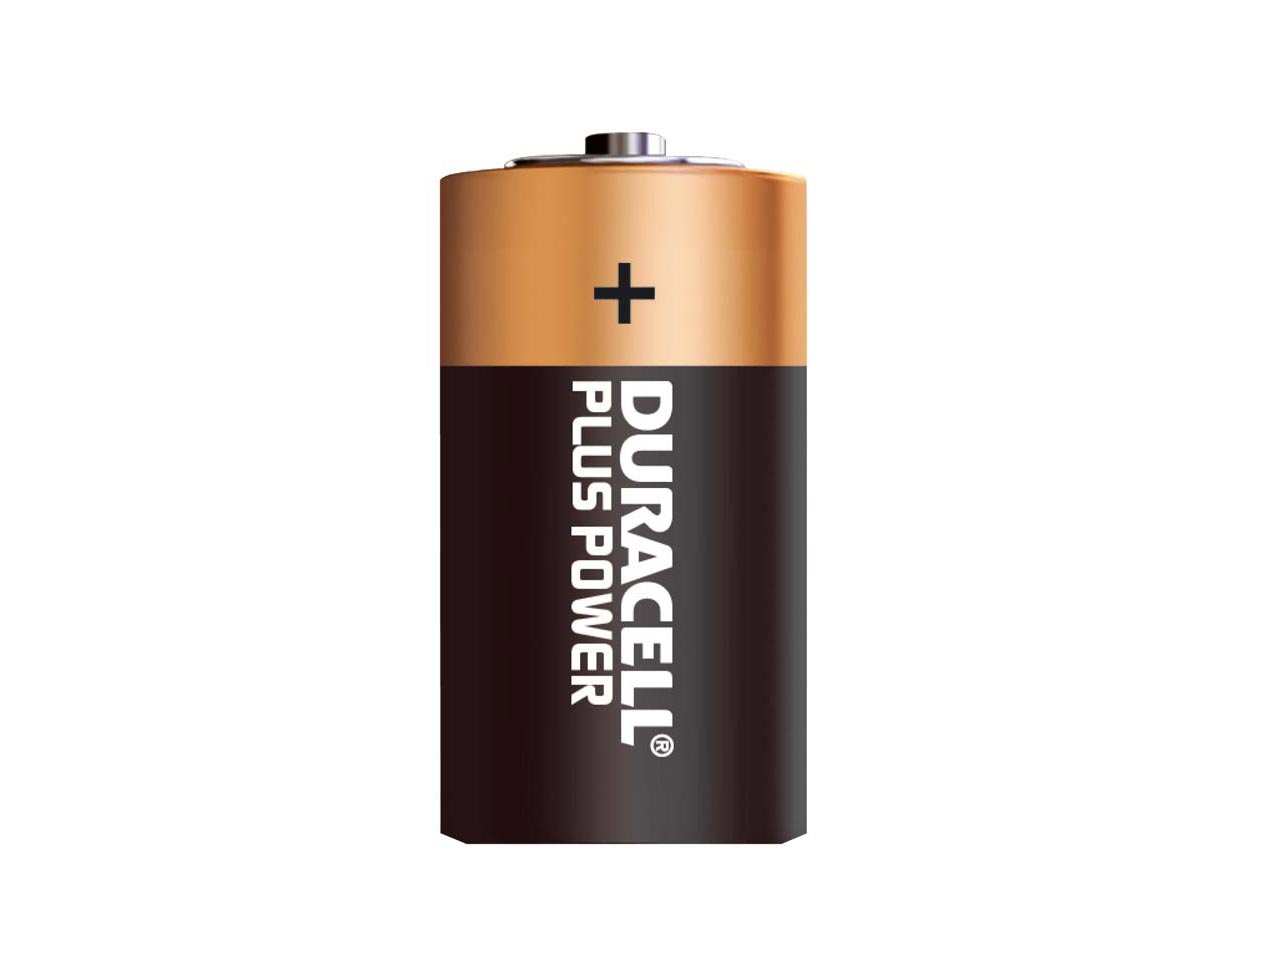
\includegraphics[width=6cm, height=6cm] {Bateries/pilaalcalina.jpg}
    \caption{Bateria o pila alcalina.}
\end{figure}

\subsection{Bateries d'àcid-plom}
Són els acumuladors més comuns fins ara en el món de l’automoció. Aquestes bateries estan formades per dos elèctrodes de plom. Durant el procés de càrrega el sulfat de plom de l’interior perd electrons i es redueix així en plom metall en el seu pol negatiu, mentre que en el pol positiu es forma l'òxid de plom. De la mateixa manera, durant el procés de descàrrega s’inverteix el procés i serà el moment en el que l’òxid de plom format en el pol positiu es transformi un altre cop en sulfat de plom, així com el plom elemental del pol negatiu s’oxidarà per convertir-se igualment en sulfat de plom. Aquest procés genera l’intercanvi d’electrons que aprofitarem per generar energia elèctrica mitjançant un circuit elèctric.

El principal avantatge de les bateries d’àcid-plom és el seu cost, així com una simple fabricació en sèrie. Per contra, són bateries que no es poden sotmetre a sobrecàrregues o descàrregues intenses, són extremadament contaminats, no es caracteritzen per una densitat d’energia massa alta i són molt pesades.

Hem de saber que els acumuladors d’àcid-plom no duren tota la vida, aquestes bateries formen cristalls i serà aleshores quan els processos de carrega-descarrega deixaran d’actuar correctament. Quan això succeeixi no tindrem un altre remei que canviar la bateria, això es coneix com una bateria sulfatada.
\bigskip \bigskip
\begin{figure}[H]
	\centering
    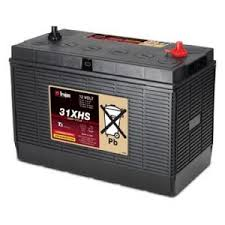
\includegraphics[width=6cm, height=6cm] {Bateries/acidplom.jpg}
    \caption{Bateria d'àcid-plom.}
\end{figure}

\subsection{Bateries de niquel ferro (NI-FE)}
Uns acumuladors formats per uns tubs fins enrotllats per làmines d’acer niquelat formen aquestes bateries. En l’interior dels tubs s’utilitza hidròxid de níquel i com electròlit una barreja de potassa càustica en aigua destil·lada. Aquests acumuladors poden carregar i descarregar perfectament sense efecte memòria ja que formen cristalls de ferro que conserven els elèctrodes en els processos. 

Els acumuladors de níquel ferro són fàcils de fabricar i a un preu baix. A més a més són molt menys contaminants que la resta d’acumuladors, se'ls hi estima una vida útil de més de 80 anys i poden funcionar en qualsevol temperatura damunt l'escorça de la terra. El seu principal inconvenient és un rendiment de només el 65\%. Actualment encara podem trobar algunes funcionant, per emmagatzemar energia generada per plaques solars o turbines eòliques. Per les seves similituds, es diu que les bateries de grafè han ressuscitat aquest tipus de bateries de níquel ferro, encara que això sí, millorant l’inconvenient del rendiment.
\bigskip
\begin{figure}[H]
	\centering
    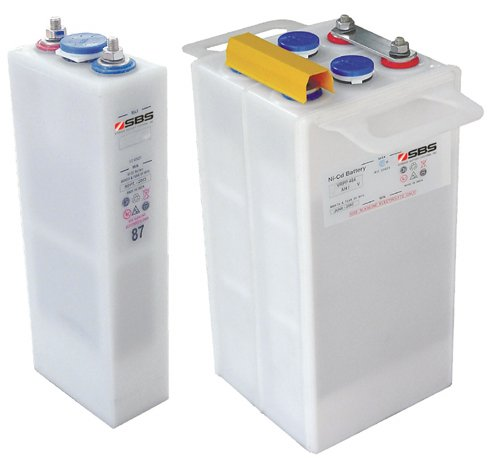
\includegraphics[width=7cm, height=7cm] {Bateries/niquelferro.jpg}
    \caption{Bateria de níquel-ferro}
\end{figure}
\newpage

\subsection{Bateries de níquel-hidrur (Ni-MH)}
Acumuladors que empren un ànode d’hidròxid de níquel i un càtode que està format per una aliatge d’hidrur metàl·lic. Uns acumuladors en els que no preocupen tant la seva càrrega per l’efecte memòria ja que l’aguanten millor que els anteriors. Per contra, no poden ser utilitzades a baixes temperatures ja que perden molt rendiment.

Aquesta classe d’acumuladors de níquel-hidrur són perfectament recarregables i han estat les pioneres en la utilització de vehicles elèctrics. \newline També en l’electrònica de gran consum en forma de pila recarregable, que requereix d'un carregador específic.
\begin{figure}[H]
	\centering
    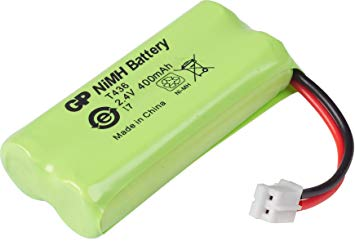
\includegraphics[width=6cm, height=6cm] {Bateries/niquelhidrur.jpg}
    \caption{Bateria de níquel-hidrur.}
\end{figure}

\subsection{Bateries de liti}
Els acumuladors de liti són coneguts actualment com els de major rendiment. La principal competència per a les noves bateries de grafè. Són les utilitzades en l'electrònica de gran consum com tauletes i mòbils intel·ligents, per les seves petites dimensions, reduint el seu pes i donant un excel·lent rendiment fins ara en comparació amb la resta de bateries del mercat.

\subsubsection{Bateries d'ions de liti (Li-Ion)}
Els acumuladors d'ions de liti s’han convertit en els més utilitzats per a dispositius electrònics. Gràcies a la seva sal de liti emprada com electròlit genera la reacció química per fer corrent elèctric. Les bateries d'ions de liti destaquen per la seva alta densitat energètica, acumuladors petits i lleugers amb elevada unitat de càrrega, i per un mínim efecte memòria, és a dir, permeten càrregues i descàrregues sense veure afectat el rendiment de l’acumulador. De totes maneres, en aquesta classe de bateries no tot són avantatges. La seva vida útil es considera mitja, no s’estima que aguantin més de tres anys aproximadament, i la seva duració en les principals aplicacions d'electrònica no és superior a un dia per l’habitual. 
\begin{figure}[H]
	\centering
    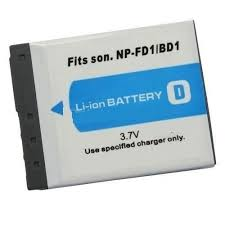
\includegraphics[width=5cm, height=5cm] {Bateries/Li-ion.jpg}
    \caption{Bateria d'ions de liti.}
\end{figure}

\subsubsection{Bateries de polímer d'ions de liti (LiPo)}
Els acumuladors de polímer de liti són una variació de les anteriors. Amb una densitat energètica superior i millores en la tassa de descàrrega. Tot i ser una classe de bateries que milloren les d'ions de liti el seu principal inconvenient és que queden pràcticament inútils si es descarreguen per sota del seu mínim de 3V.
\begin{figure}[H]
	\centering
    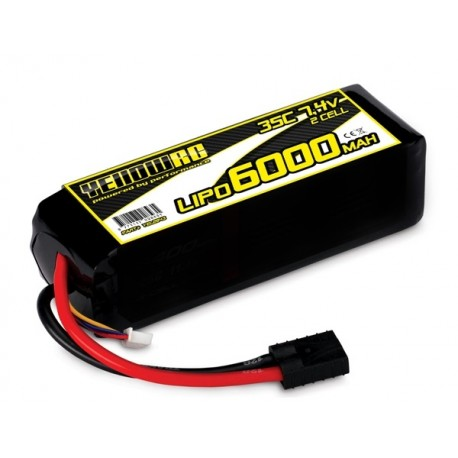
\includegraphics[width=6cm, height=7cm] {Bateries/lipo.jpg}
    \caption{Bateria de polímer d'ions de liti.}
\end{figure}

\subsection{Bateries de grafè}
Aquestes bateries encara estan en desenvolupament. No s’ha acabat de trobar encara un equilibri que pugui estabilitzar el pros i els contres \newline d’aquest tipus de bateries. Els polímers de grafè són un nano material format per carboni pur amb àtoms disposats en patró hexagonal. En el fons es tracta d’un material molt similar al grafit, però amb major duresa, flexibilitat i elasticitat. No obstant, el punt més interessant d’aquest nano-material transparent és la seva altíssima conductivitat elèctrica, a més a més de la seva capacitat per generar electricitat al ser assolits per la llum. 
En termes pràctics, les bateries de grafè tenen una velocitat de càrrega molt més ràpida i una densitat d’energia moltíssim més elevada que el que mai podran oferir les bateries d’ions de liti. També un altre punt a tenir en compte és que són molt menys pesades que les bateries habituals. Això porta lloc a un gran interès sobre aquestes bateries en el món de l’automoció, ja que es pot arribar a reduir el pes de la bateria fins a un 75\% a més a més de donar totes les característiques esmentades anteriorment.
\begin{figure}[H]
	\centering
    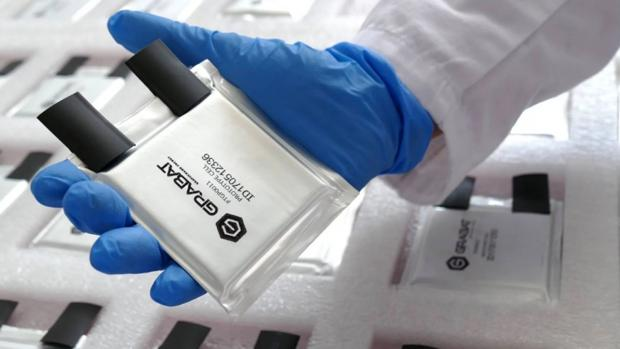
\includegraphics[width=9cm, height=7cm] {Bateries/grafeno.jpg}
    \caption{Bateria de grafè.}
\end{figure}                                    

\section{Bateries de liti com a font d'energia per al nostre vehicle elèctric}
En primer lloc el que cal saber per entendre millor aquest tipus de bateries és tindre un petit coneixement de les característiques que permet el liti. El liti és un metall alcalí, inflamable, blanc platejat, dúctil i molt poc pesat que es caracteritza per corroir-se amb rapidesa quan entra en contacte amb l’aire. No existeix en estat lliure en la naturalesa encara que si està present en compostos com en l'escorça terrestre. La presència del liti en la naturalesa és molt comuna ja que es troba en 65 parts per milió de l'escorça terrestre. A més a més el liti no es pot submergir sota l’aigua perquè podria cremar i el contacte amb la pell podria ocasionar lesions, pel que és indispensable que el fabricant de les bateries de liti compti amb materials i mètodes de fabricació que compleixin la normativa i exigències vigents. Encara que nombroses investigacions afirmin que el liti té propietats molt interessants que encara no s’han estudiat en profunditat, actualment l’ús principal del liti és per a les bateries de liti, oferint excel·lents propietats en comparació amb altres tipus de bateries molt comunes en el mercat.

Les bateries de liti, es caracteritzen per carregar-se més ràpid, durar més, comptar amb una major vida útil i oferir més densitat energètica, pel que en menys espai es pot obtenir una major autonomia i treure-li més partit a les bateries de liti.

\begin{figure}[H]
	\centering
    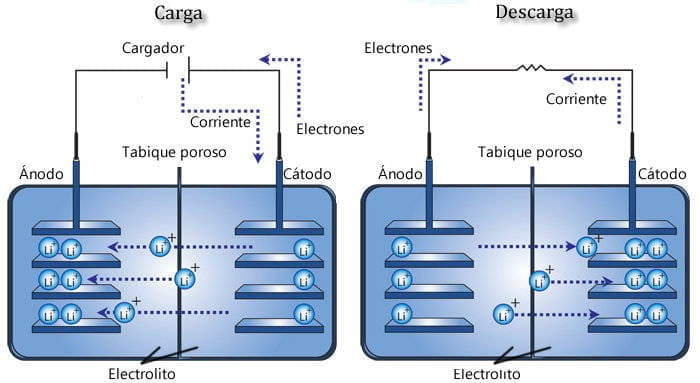
\includegraphics[width=\textwidth, height=7cm] {Bateries/cargadescargalitio.jpg}
    \caption{Funcionament d'una bateria de liti}
\end{figure}

Existeixen tres tipus de bateries de liti:
\begin{itemize}
    \item Bateries d’òxid de cobalt/liti: Tenen el benefici de l’alta densitat \newline d’energia, que encara que a vegades pugui comportar problemes de seguretat, solen tractar-se de bateries de gran durabilitat.
    \item Bateries de liti/òxid de magnesi: Es tracta de la bateria més emprada pel seu alt nivell de seguretat, però el seu rendiment no sempre és eficient quan s’experimenten altes temperatures.
    \item Bateries de liti/fosfat de ferro: Es tracta de la bateria amb les majors característiques de seguretat amb una llarga vida útil, de més de 2000 cicles. 
\end{itemize}

\subsection{Bateries d'ions de liti}
Les bateries d'ions de liti són un dispositiu dissenyat per a \newline l'emmagatzemament d’energia elèctrica que empra com electròlit una sal de liti que aconsegueix els ions necessaris per a la reacció electroquímica reversible que té lloc entre el càtode i l'ànode.

Les propietats de las bateries de Li-Ion, com la lleugeresa dels seus component, la seva elevada capacitat energètica i resistència a la descarrega, juntament amb el poc efecte memòria que sofreixen o la seva capacitat per a funcionar a un elevat nombre de cicles de regeneració, ha permès dissenyar acumuladors lleugers, de petita mida i variades formes, amb un alt rendiment, especialment adaptats a les aplicacions de la indústria electrònica de gran consum. Des de la primera comercialització d’un acumulador basat en la tecnologia Li-Ion a principis dels anys 90, el seu ús s’ha popularitzat en aparells com telèfons mòbils, agendes electròniques, ordinadors portàtils i lectors de música.

No obstant, la seva ràpida degradació i sensibilitat a les altes temperatures, que pot resultar en la destrucció per inflamació o inclús explosió, requereixen, en la seva configuració com a producte de consum, la inclusió de dispositius addicionals de seguretat, resultant en un cost superior que ha limitat l’extensió del seu ús a altres aplicacions.

En el context del creixent encariment de combustibles derivats del petroli, la industria de l'automòbil ha anunciat el seu desenvolupament, proliferació i comercialització de vehicles amb motors elèctrics basats en la tecnologia de les bateries d’ions de liti, amb els que es pugui disminuir la dependència energètica d’aquestes fonts a la vegada que es manté la baixa emissió de gasos contaminants.

\subsection{Bateria de polímer de liti (LiPo)}

Les bateries de polímer d'ions de liti són piles recarregables, compostes generalment de vàries cel·les secundàries idèntiques en paral·lel per augmentar la capacitat del corrent de descàrrega, i estan sovint disponibles en sèries de paquets per augmentar el voltatge total disponible.

Les bateries LiPo funcionen seguint el mateix principi que les bateries d'ions de liti, l’intercanvi d’electrons entre el material de l'elèctrode \newline negatiu i el material de l'elèctrode positiu mitjançant un conductor. Per evitar que els elèctrodes es toquin directament, es col·loca entre ells un material amb porus microscòpics, que permeten tan sols als ions de liti (i no a les partícules dels elèctrodes) migrar d’un elèctrode a l'altre.

Les bateries LiPo estan classificades pel numero de cel·les “S” pel qual estan formades. Així una bateria 4S estaria composta per 4 sub-bateries connectades en sèrie. A més a més la capacitat d’aquestes bateries queda indicada en “mAh”. A major nombre de mil·liamperes (mAh) més capacitat de càrrega. Quan parlem d’una bateria amb una capacitat de 2200 mAh estem dient que aquesta bateria és capaç de descarregar a 2,2 A en una hora.

\subsection{Avantatges i desavantatges de les bateries LiPo}

Els principals avantatges i desavantatges que tenen aquestes bateries són els següents:
\begin{itemize}
    \item No presenta sulfatació.
    \item Alta densitat de càrrega.
    \item No existeix la necessitat d'una càrrega prolongada quan són noves.
    \item Índex d'auto-descàrrega baix.
    \item Són bateries que generen un menor impacte en el medi ambient.
    \item Varietat de models disponibles tant en càrrega com en mida, un fet molt important que li dona versatilitat.
    \item No requereixen de tant manteniment com altres bateries, no necessiten descàrregues periòdiques ja que no presenten efecte memòria.
\end{itemize}

Però no tot són avantatges. També presenten una sèrie de desavantatges a tenir molt en compte:
\begin{itemize}
    \item Envelliment: Les bateries d'ions de liti estan exposades a envelliment per diversos motius. Un excés de temperatura, un elevat nombre de càrregues i descàrregues que provoca una degradació, també la provoca (i en això és on es diferencia d'altres tipus de bateries) el deteriorament durant el temps que estan emmagatzemades amb càrrega. 
    \item Requereixen protecció: Les cel·les d'ions de liti no són tan robustes com altres tecnologies recarregables. Han de tenir un sistema de protecció davant de sobrecàrregues i descàrregues profundes, temperatura...
    \item Cost: Les bateries LiPo tenen un cost de fabricació més alt que altres bateries.
    \item Rapid disassembly: Aquest és un dels problemes en els que més es treballa per evitar. Es pot donar per la presència de partícules metàl·liques microscòpiques que arriben a curtcircuitar la cel·la, però aquesta causa és cada cop més rara ja que els fabricants de bateries s'enfoquen en l'eliminació d'aquestes partícules, encara que l'eliminació total d'aquestes és impossible. Però el verdader problema està en que els curtcircuits es provoquin dins la cel·la, allà les proteccions externes són ineficaces per parar la reacció que es produeix. Si degut a un defecte en la bateria o a un mal ús d'aquesta la bateria s'escalfa en excés, aquesta temperatura pot afectar a la integritat de la capa d'aïllament d'una de les cel·les. Si aquesta capa falla es produeix un curtcircuit en que les temperatures poden arribar als 500ºC i la cel·la pot incendiar-se o explotar. Això a la vegada pot afectar a les cel·les properes i pot originar una reacció en cadena. 
\end{itemize}

\subsection{Riscs en l'ús de bateries LiPo}

El funcionament i la qualitat d'una bateria LiPo ve determinat pel \newline voltatge donat per la cel·la i la temperatura d'aquesta. Aquests són els factors més importants a tenir present sobre una bateria LiPo. 

\subsubsection{Riscs en la sobrecàrrega}
Si el voltatge de càrrega s'incrementa per sobre del seu màxim aconsellable de 4,2V provoca que circuli un corrent excessiu, el que deriva als següents problemes:
\begin{itemize}
    \item Sobreescalfament: Un excés de corrent en la càrrega incrementa \newline l'escalfament de la cel·la. 
    \item Formació de plaques de liti: Quan el corrent de càrrega resulta excessiu , els ions de liti no s'acomoden suficientment ràpid entre els estrats d'intercalació de l'ànode, sinó que s'acumulen en la superfície de l'ànode formant una placa de liti metàl·lic. Aquesta formació de plaques es tradueix en que després en la descàrrega hi haurà una quantitat menor d'ions de liti lliures suposant una pèrdua de capacitat de la bateria. 
\end{itemize}

\subsubsection{Riscs en la sobre descàrrega}
De la mateixa manera que sotmetre a la cel·la a un voltatge de càrrega excessiu causa problemes el descarregar-la en excés genera un molt important que és la descomposició dels materials dels elèctrodes.
\begin{itemize}
    \item Càtode: Mantenir les cel·les a voltatges inferiors de 2 volts de manera prolongada provoca la descomposició gradual del càtode. Durant aquesta descomposició s'allibera oxigen de l'òxid de liti tot provocant un augment de la pressió dins de la cel·la. Es pot arribar a manifestar d'una forma violenta si no disposen d'una sortida més controlada.   
   \item Ànode: El col·lector de corrent de l'ànode de coure es dissol en \newline l'electròlit. Aquest provoca que augmenti l'auto descàrrega de la bateria i que quan s'intenti recarregar la cel·la, en el moment que el seu voltatge augmenti en dos volts, els ions de coure que s'han dissolt en l'electròlit es precipitaran com coure metàl·lic i no necessàriament es dipositaran en el dipòsit de coure de l'ànode. Això és un comportament de risc que pot causar en última instància un curtcircuit entre elèctrodes.

\end{itemize}

\subsubsection{Riscs a baixes temperatures de funcionament}
L'índex de reaccions químiques està relacionat amb la temperatura. \newline La reducció de la temperatura de funcionament d'una cel·la implica reduir el nombre de reaccions químiques que es produeixen dins d'aquesta. Això es tradueix en una reducció del corrent que pot suportar la cel·la durant la càrrega i la descàrrega. Implica una pèrdua de potència útil de la cel·la i un augment del dany generat a aquesta durant la càrrega. Si es carrega la cel·la amb un corrent superior a l'admissible els ions de liti en comptes d'inserir-se entre els estrats es dedicaran a formar plaques de liti.


\subsubsection{Riscs a altes temperatures de funcionament}
Operar a temperatures excessives produeix una sèrie de problemes, la majoria relacionats amb la destrucció de la cel·la. Una temperatura elevada provoca un augment del nombre de reaccions químiques que es produeixen en la cel·la i fa que el corrent de la cel·la augmenti. Això que en principi sembla bo no ho és ja que un augment en el corrent ve de la mà amb un augment de la potència dissipada en la resistència interna de la cel·la, potència que es dissipa en escalfor i fa que encara augmenti més la temperatura. De no controlar-ho a la cel·la succeiria una fuga tèrmica.

\subsubsection{Fuga tèrmica}
La primera etapa en una fuga tèrmica és la destrucció de la capa SEI\footnote{Solid Electrolyte Interface} en l'ànode degut a un sobreescalfament d'aquesta o a una perforació. El sobreescalfament pot estar produït per un excessiu corrent, una sobrecàrrega de la cel·la o per una temperatura ambient massa elevada. La destrucció d'aquest estrat comença a una temperatura relativament baixa, 80ºC. Un cop que es danya la capa l'electròlit reacciona amb l'ànode de carboni tal i com succeeix durant la formació original de la capa SEI, ara d'una manera més descontrolada. Considerant que és una reacció exotèrmica contribueix a aquest augment de temperatura de la cel·la. 

A mesura que la temperatura de la cel·la creix el calor generat en l'ànode provoca la descomposició dels dissolvents orgànics emprats en l'electròlit alliberant aquests gasos inflamables com el metà. Aquesta descomposició sol començar als 110º, això depèn de la naturalesa de l'electròlit on en alguns casos pot arribar a començar als 70º. El gas generat s'acumula augmentant la pressió dins la cel·la. Encara que la temperatura de la cel·la augmenti per sobre del punt d'inflamació no s'inicia la combustió degut a que no hi ha oxigen. Les cel·les solen estar equipades amb algun mecanisme capaç d'alliberar pressió de la cel·la sense posar a aquesta en risc, evitant així l'explosió. Però una vegada els gasos són alliberats a l'atmosfera i a aquesta temperatura cremen.

Als 135º aproximadament es fon el separador provocant un curtcircuit entre els dos elèctrodes. L'escalfor generat en aquest curtcircuit provoca la descomposició de l'òxid del càtode el que allibera oxigen, tot permetent que els gasos i l'electròlit que queden a l'interior de la cel·la cremin,. Aquesta combustió eleva tant la temperatura i la pressió de la cel·la que aquesta explota. La temperatura a la qual es sol descompondre el càtode és d'aproximadament 200ºC.

\subsection{Seguretats a tenir en compte en les bateries LiPo}

Les bateries LiPo són bastant delicades. Si bé una bateria amb bon ús i bon manteniment pot arribar a realitzar més de 300 cicles de càrrega i descàrrega, una bateria mal cuidada pot no arribar ni als 50 cicles. A més a més, el seu ús incorrecte, en especial les sobrecàrregues, pot produir que les bateries LiPo cremin. Per això, per treballar amb bateries de forma segura i per allargar la vida útil de les mateixes, és important seguir uns certs consells:

\begin{itemize}
    \item Mai deixar desateses les bateries mentre carreguen, poden cremar. \item Carregar-les en un lloc on no hi hagi materials inflamables. 
    \item Necessari carregar-les amb un carregador específic.
    \item Mai s'ha de deixar que els terminals entrin en contacte entre ells, ja que això provocaria un curt-circuit i podria fer que la bateria \newline s'incendiés.
    \item Deixar refredar les bateries a la temperatura ambient després de fer-les servir abans de carregar-les.
    \item Mai carregar les bateries per sobre del voltatge indicat pel fabricant. Hi ha perill que cremin. Tampoc s'han de carregar en llocs molt freds (menys de 5ºC) ni molt calents. La temperatura ideal de funcionament d'una bateria LiPo es troba entre els 30 i 40ºC. Per sota, la bateria no treballa al 100\% i per sobre de 60ºC la bateria ja comença a malmetre's. 
\end{itemize}
La millor forma d'emmagatzemar les bateries durant molt temps és deixant-les a un 40\% de la seva càrrega. Ha de ser un lloc sec i a una temperatura entre 5 i 25ºC.Existeixen fundes especials ignífugues que s'utilitzen per emmagatzemar les bateries de forma segura.

Mai s'ha de fer servir una bateria que es vegi danyada o voluminosa. Si en qualsevol moment s'observa que la bateria LiPo s'infla o derrama líquid, cal desconnectar-la i observar-la durant uns 10 minuts o 20 minuts en un lloc segur. Això podria provocar l'ignició de la bateria degut als components químics que entren en contacte amb l'aire.

\subsection{Característiques de la càrrega de bateries LiPo}
Per seguretat i per prolongar la vida de la bateria hem de tenir en compte com es realitza una càrrega segura d'una bateria d'ions de liti. A continuació es mostrarà el procés de càrrega d'una cel·la d'ions de liti, en una càrrega genèrica no una específica.

Concretament estem parlant de bateries de Li-ion fabricades amb els materials de càtode tradicionals de cobalt, níquel, manganès i alumini de càrrega típicament a 4.2V/cel·la. La tolerància es +/- 50mV/cel·la. 

Un dels principals conceptes que s'han de tenir en compte és que en les bateries de liti els voltatges de tall no tenen una flexibilitat com altres bateries. En augmentar el voltatge també s'augmenta la capacitat, però anar més enllà de l'especificació pot sobrecarregar la bateria. Els circuits de protecció incorporats en el paquet no permeten excedir el voltatge establert.
Voltatges més alts provocarien estrès a la bateria, comportant a una reducció de la seva vida útil. És més preocupant el problema de seguretat que pot comportar aquest excés de tensió.

A continuació es mostrarà una gràfica en la que es poden veure les diferents fases de càrrega de la cel·la.

\begin{figure}[H]
	\centering
    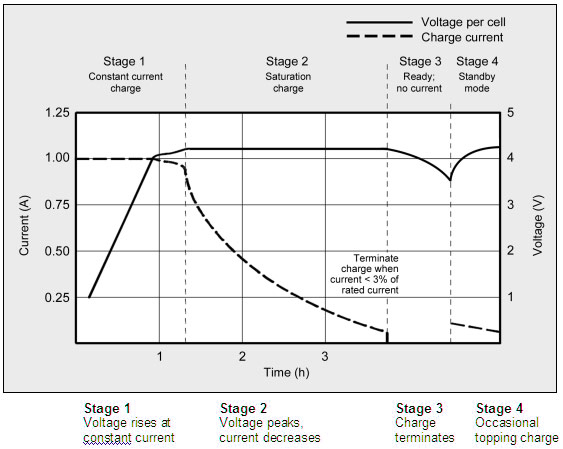
\includegraphics[width=\textwidth, height=8cm] {Bateries/cargabatlipo.jpg}
    \caption{Etapes de càrrega d'una bateria LiPo.}
\end{figure}

A l'etapa 1 es veu com la velocitat de càrrega d'una bateria típica és d'entre 0,5 i 1A. La càrrega complerta es produeix quan la bateria arriba al llindar de voltatge i el corrent cau al tres per cent del corrent nominal. Aquest punt es pot apreciar al final de l'etapa 2 i inici de l'etapa 3. En lloc de càrrega lenta, alguns carregadors apliquen una càrrega màxima quan la tensió cau a 4.05V/cell (etapa 4).

El temps total de càrrega és aproximadament d'unes tres hores en funció del mètode de càrrega. Quan la bateria queda completament carregada la seva temperatura pot augmentar fins a 5ºC. Si s'augmenta el corrent de càrrega la bateria no es carregarà abans, sinó que arribarà abans al pic de tensió. No obstant  l'etapa 2 (saturació) requerirà més temps.

Una bateria de liti no pot absorbir la sobrecàrrega i és precís que quan s'arribi a la càrrega complerta el corrent sigui tallat. Si aquest continua es poden formar plaques de liti metàl·lic que són un factor de perill ja que poden causar curtcircuits. També augmenta l'estrès de la bateria si es manté durant un bon temps el voltatge de pic de 4,2V.

Un cop que la càrrega es termina, el voltatge de la bateria comença a disminuir, el que alleuja l'estrès de tensió. Amb el temps, el voltatge de circuit obert s'assentarà entre 3,6 i 3,9V/cel·la. S'ha de tenir en compte que una bateria de Li-ion que ha rebut una càrrega totalment saturada mantindrà la tensió més alta que una on la seva càrrega ha estat ràpida i sense càrrega de saturació.

La següent gràfica mostra la relació entre tensió, corrent i capacitat que succeeix en la càrrega d'una cel·la.

\begin{figure}[H]
	\centering
    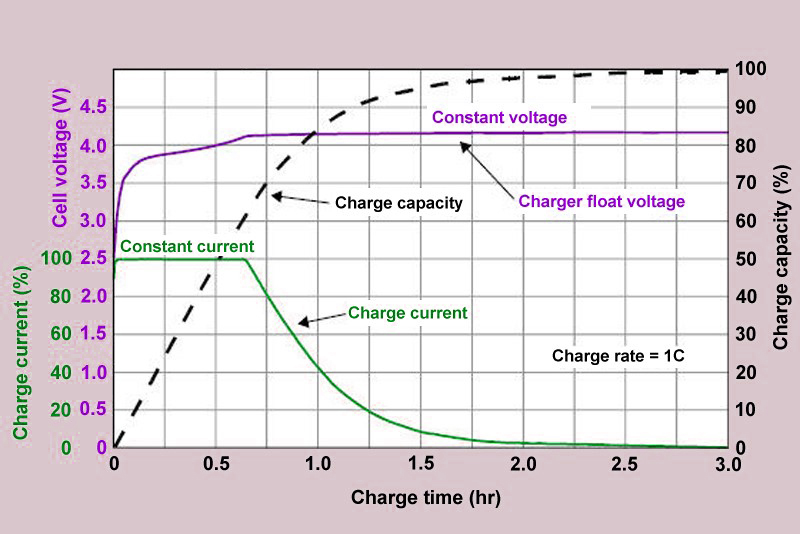
\includegraphics[width=\textwidth, height=7cm] {Bateries/VICgrafica.jpg}
    \caption{Evolució del voltatge, el corrent i la capacitat en la càrrega d'una bateria LiPo.}
\end{figure}

Alguns carregadors apliquen una breu càrrega d'anivellació per compensar la petita auto-descàrrega de la bateria i el consum del circuit de protecció. El carregador pot arrencar quan el voltatge de circuit obert de la cel·la cau a 4.05V i tanca de nou a 4.2V.

Un dispositiu portàtil ha d'estar apagat durant la càrrega. Això permet que la bateria arribi a un voltatge llindar establert sense problemes, i permet acabar la càrrega amb corrent baix. Una càrrega parasitària confon el carregador mitjançant la pulsació de la tensió de la bateria i altera la mesura del corrent en la fase de saturació.

Les bateries d'aquest tipus treballen amb seguretat dins dels límits fixats però es tornen inestables si es sobrecarreguen amb una tensió superior a l'especificada. Es comencen a formar plaques de liti en l'ànode mentre que en el càtode es produeix un material oxidant, perd estabilitat i produeix CO2. Si no s'activa cap mecanisme de seguretat pot desencadenar en una fuga tèrmica. 

\subsection{Característiques de la descàrrega de bateries LiPo}

Les cel·les d'una bateria de liti no han de ser descarregades massa, per norma l'equip hauria d'interrompre la descàrrega quan el voltatge d'una cel·la arribi als 3V. Si el seu voltatge baixa dels 2.7V el circuit de protecció de la bateria posarà la bateria en mode espera i una recàrrega ja no serà possible amb la majoria dels carregadors comercials. No s'han de recarregar cel·les on la tensió hagi caigut per sota dels 1,5V doncs poden haver-se format derivacions de coure en l'interior de l'ànode i poden produir un curtcircuit.

A continuació es mostrarà una gràfica en la que es pot veure la relació del voltatge en funció de la capacitat durant la descàrrega a diferents intensitats.

\begin{figure}[H]
	\centering
    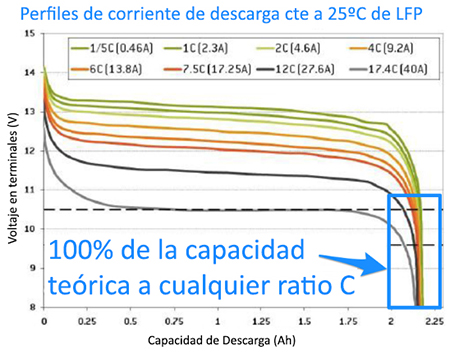
\includegraphics[width=10cm, height=10cm] {Bateries/graficadescargabatlipo.jpg}
    \caption{Descàrrega d'una bateria LiPo a diferents intensitats.}
\end{figure}

\chapter{Gestió de bateries: BMS}
\label{chap:BMS}


Un BMS (Battery Management System) és un sistema electrònic que \newline s'encarrega de gestionar una bateria, des de la càrrega i la descàrrega com el balanceig i el control de la temperatura. Així doncs, ha de poder contemplar certs paràmetres d'una bateria per maximitzar el seu rendiment, mantenir o allargar la seva vida útil, en el nostre cas ens centrarem amb bateries LiPo que són un tipus de bateries amb molta densitat energètica que necessiten disposar d'un BMS.

Un BMS està composat per un hardware i un software que controlen la càrrega i la descàrrega d'una bateria garantint al mateix temps una operació confiable i segura. Això implica el control dels nivells de corrent i tensió, de les condicions de càrrega i descàrrega, de la limitació de la finestra d'operació respecte del SOC i/o la temperatura, de la gestió tèrmica, del balanç en tensió entre les cel·les, etc. Un apropiat sistema de gestió capaç de predir la màxima energia i potència disponible per una connexió i desconnexió segura de les cadenes farà que millorin el seu ús. Un BMS no només controla les funcions d'emmagatzemament per optimitzar la vida útil, eficiència i seguretat del dispositiu, si no que proveeix una precisa estimació dels estats de la bateria per a la gestió energètica. 

\newpage

Els BMS compten amb dos importants enfocaments operacionals, monitoratge i control, que no poden ser separats durant l'operació, per exemple, per garantir un apropiat, ràpid i precís control de la càrrega i descàrrega de les bateries és necessari un sistema de monitoreig que analitzi el voltatge, el corrent, la temperatura interna, SOC i SOH (State of Health), tot protegint la bateria contra situacions perilloses com sobrecàrregues i descàrre- \newline gues profundes.

\begin{figure}[H]
	\centering
    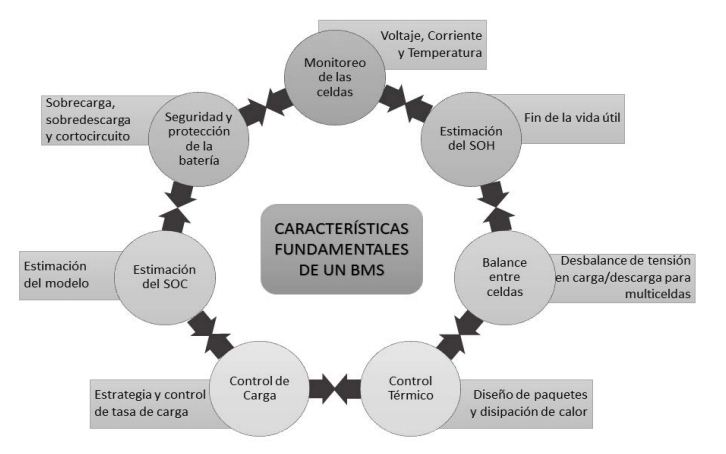
\includegraphics[width=\textwidth, height=10cm] {BMS/diagramabms.png}
    \caption{Característiques fonamentals d'un BMS.}
\end{figure}

\section{Perquè es necessita un BMS?}
El motiu principal de la necessitat d'un gestor de bateries és el fet de que les bateries encara han de millorar molt tecnològicament i han de ser més segures. La majoria de les bateries funcionen prou bé dintre d'uns certs marges, fóra d'aquests la bateria perilla. El problema principal de les bateries de liti és que són molt intolerants a sobrecàrregues i descàrregues profundes, si aquestes coses no es protegeixen no només perilla la bateria, sinó que si la bateria està instal·lada dins d'un vehicle i explota podria provocar greus conseqüències. És per això que si un òptim BMS que controli les condicions operacionals de la bateria per a prolongar la seva vida útil i garanteixi la seva seguretat a través de l'estimació dels paràmetres SOC i SOH, és molt important. 
Tot això és possible gràcies a que el BMS posseeix característiques per al control i monitoreig de l'estat de cada cel·la i així conèixer el seu estat actual, predir la seva capacitat i controlar l'intercanvi energètic. Encara aquí la precisió en l'estimació juga un paper fonamental, fins al punt de convertir-se en un factor normatiu que posseeix diferents conflictes: precisió dels sensors i sistemes d'adquisició de dades, necessitat d'arribar a un objectiu tècnic donat, esforç degut al rendiment de la bateria, qualitat dels models i algorismes emprats. Per tant, una confiable estimació del SOC i SOH no només és \newline  necessària contra descàrregues profundes o sobrecàrregues, prolonga la vida de la bateria i la prediu.  

És vital que tot BMS porti sensors de temperatura per a monitorar en tot moment les cel·les. Ja sabem que les bateries de liti tenen un alt risc si es surten dels límits que permet el fabricant. És per això que cal controlar la temperatura de les cel·les per tractar d'evitar que es puguin arribar a encendre i que malmetin el BMS. Si per exemple una cel·la d'una bateria està carregant-se per sobre del seu voltatge, aquesta comença a augmentar la seva temperatura ja que hi està circulant més corrent. Si no s'aplica cap mesura, la cel·la pot arribar a incendiar-se, provocant inclús danys a les altres cel·les i, en el pitjor dels casos, cremar tota la bateria o explotar. Això comporta que s'estableixin unes certes mesures de seguretat i no hi ha millor opció que el BMS. En el fons s'encarrega de protegir les bateries i protegir a l'individu que estigui manipulant-les.

\section{Quins elements té en compte un BMS?}
Un BMS pot controlar l'estat de la bateria tal com es representen diversos elements, com ara:
\begin{itemize}	
	\item Voltatge: tensió total, voltatges de cel·les individuals, tensió mínima o màxima de cel·les o tensió de taps periòdics.
    \item Temperatura: temperatura mitjana, temperatura d'entrada de refrigerant, temperatura de sortida del refrigerant o temperatures de cel·les individuals.
    \item Estat de càrrega (SOC) o profunditat de descàrrega (DOD), per indicar el nivell de càrrega de la bateria.
    \item Estat de salut (SOH), una mesura diferentment definida de la capacitat restant de la bateria com a percentatge de la capacitat original.
    \item Estat de potència (SOP), la quantitat de potència disponible per a un interval de temps definit, tenint en compte el consum d'energia actual, la temperatura i altres condicions.
    \item Fluid refrigerant: per a bateries d'aire o de refrigeració fluida.
    \item Corrent : actual dins o fora de la bateria. 
    \item frenada regenerativa: controlarà la recàrrega de la bateria redirigint l'energia recuperada de tornada al paquet de bateria.
    \item Corrent màxim de càrrega com a límit de corrent de càrrega.
    \item Corrent de càrrega màxim com a límit de corrent de descàrrega.
	\item Energia [kWh] lliurada des de l'última càrrega o cicle de càrrega.
	\item Impedància interna d'una cel·la (per determinar la tensió del circuit obert).
	\item Càrrega [Ah] lliurada o emmagatzemada (de vegades aquesta característica es diu comptador Coulomb).
	\item Energia total lliurada des del primer ús.
	\item Temps total de funcionament des del primer ús.
	\item Nombre total de cicles.
    \item Eliminant energia de les cel·les més carregades connectant-les a una càrrega (com mitjançant reguladors passius).
\end{itemize}

\section{Quins càlculs realitza un BMS?}
Un BMS pot calcular valors basats en els ítems d’abaix, com:
\begin{itemize}
	\item Corrent de càrrega màxim com a límit de carrega de corrent (CCL charge current limit).
	\item Corrent de descàrrega com a límit de descarrega de corrent (DCL discharge current limit).
	\item Energia (KWh) entregada des de l’última càrrega o cicles de càrrega.
	\item Impedància interna d’una cel·la (per determinar el voltatge en circuit obert).
	\item Càrrega (Ah) entregada o emmagatzemada (a vegades aquesta característica és nombrada comptador Coulomb).
	\item Energia total entregada des del primer ús.
	\item Nombre total de cicles.
\end{itemize}

Hi ha una gran llista de funcions que pot arribar a desenvolupar el BMS, amb l'actual electrònica i gràcies als microcontroladors és possible arribar a monitoritzar tots aquests paràmetres. No obstant, no es requereixen tenir tots aquests paràmetres per a donar un bon ús a les nostres bateries. El paràmetre que més ens interessa com a usuaris és el SOC. Amb l'estimació del SOC ja s'engloben els voltatges, temperatures i corrents. 

El SOC és l'estat de càrrega, expressat com un percentatge del total de la capacitat màxima que té. Normalment les bateries estan composades per un compost de cel·les. De la mateixa manera que es vol saber l'estat de la bateria, el BMS pot calcular l'estat de cada una de les cel·les i en funció del resultat, descarregar o carregar aquella cel·la més o menys per estabilitzar totes les cel·les de la bateria. El SOC ens permet conèixer en tot moment l'estat de les cel·les.

\section{Estat de càrrega (SOC)}
L'estimació de l'estat de càrrega és essencial per assolir el comportament òptim d'un sistema que controli vehicles elèctrics, ja que el que es vol és poder maximitzar l'utilització del motor elèctric respecte al de combustió.

L'estat de càrrega (SOC) d'una bateria o una cel·la correspon al percentatge de la seva capacitat total d'energia que encara es troba disponible en un determinat moment. No existeix una manera directa de mesurar el SOC d'una bateria degut a l'edat, el voltatge de càrrega, temperatura, velocitat de descàrrega entre altres que afecten la mesura del SOC. El desenvolupament d'una mesura de l'estat de càrrega és un procés molt complex, per la qual es defineix usualment com una estimació en lloc d'una mesura o determinació com a tal. No hi ha un únic procés adequat per a mesurar el SOC.

Un dels factors més importants que afecten a l'estimació del SOC d'una bateria és l'envelliment. Degut als cicles de càrrega i descàrrega, la capacitat de les cel·les que formen la bateria decreix amb el temps. Aquest fet indueix a actualitzar el màxim estat de càrrega disponible per a la bateria periòdicament ja que és la referència per calcular el percentatge abans mencionat. En cas de prendre com a referència el valor nominal per a la capacitat de la bateria, l'estimació pot contenir errors de pes. El procés electroquímic dins de les cel·les al carregar-se i descarregar-se sempre pren un temps finit i no sempre és menor que l'estímul elèctric que càrrega la bateria. Durant el procés de càrrega pot donar-se un pols de descàrrega i no ser realitzat per complert donant lloc a imprecisions en l'estimació del SOC. A més a més, els processos tant de càrrega com descàrrega consumeixen energia i l'energia subministradora per la bateria serà menor que l'utilitzada per a carregar-les. Aquesta proporció rep el nom d'eficiència de Coulomb i pot afectar fins a un 3\% de la capacitat disponible. 

El SOC s'entén com la quantitat de càrrega encara disponible en relació amb la capacitat de la bateria. L'estat de càrrega es calcula amb la relació entre la diferència de la capacitat nominal de la cel·la i la capacitat restant per un costat i la capacitat nominal per l'altre. L'estat de càrrega és 1 quan s'arriba a l'estat complert de càrrega i 0 després d'una descàrrega complerta.

\begin{figure}[H]
	\centering
    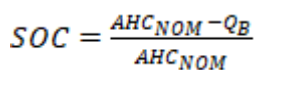
\includegraphics[width=5cm, height=3cm] {BMS/Coulombcountingformula.png}
    \caption{Fórmula elemental per al càlcul del SOC.}
\end{figure}

\begin{itemize}
    \item SOC: Estat de la càrrega de la bateria.
    \item Qb: Càrrega restant.
    \item AHCnom: Capacitat nominal (Hora - Ampere).
\end{itemize}

Abans de parlar dels mètodes més comuns per fer l'estimació del SOC d'una bateria, cal parlar d'un concepte clau en el món de les bateries i el SOC. Aquest concepte és l'histèresi. L'histèresi és la tendència d'un material a conservar les seves propietats. Les bateries estan composades per materials ferromagnètics els quals també tenen una tendència a conserver les seves propietats. En el cas de les bateries i parlant ja en els termes del BMS vindria a ser l'evolució del voltatge en el temps respecte les característiques del material de la cel·la. Com ja hem comentat prèviament dues bateries amb les mateixes característiques tècniques sobre una mateixa càrrega no es descarreguen igual.

És per això que la bateria pot estar a un mateix voltatge però a diferent capacitat. Per tant existeix un rang en el que no podem assegurar únicament amb el voltatge la capacitat. És per això que s'inclouen més variables a l'algorisme per tal d'afinar molt més el SOC.

\begin{figure}[H]
	\centering
    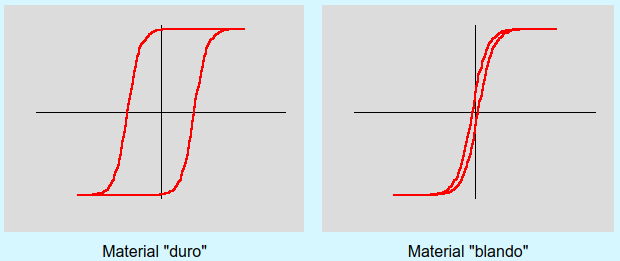
\includegraphics[width=\textwidth, height=7cm] {BMS/histeresis.png}
    \caption{Cicle d'histèresi en funció del material.}
\end{figure}

\subsection{Mètodes d'estimació per al SOC}
Existeixen diferents mètodes per a fer l'estimació del SOC. Els més comuns són els següents:

\begin{itemize}
    \item Mesura directa: Es tracta d'un mètode teòric i hipotètic ja que es basa en la hipòtesi d'un corrent de descàrrega constant. Aquest valor es multiplicat pel temps de descàrrega total de la bateria obtenint-se la capacitat de la pila de bateries. Com es fàcil d'intuir, es tracta d'un mètode inviable ja que el corrent de descàrrega és variable a la pràctica i, a més a més, els usuaris han de conèixer l'estimació del SOC sense descarregar la bateria o, al menys, abans de la descàrrega total de la mateixa.
   
    \item Mesura de la gravetat específica: També és conegut com a mesura de la densitat relativa i és necessari tenir accés a l'electròlit líquid intern de la bateria. Existeix una relació matemàtica entre la densitat de l'aigua i la d'una substància electròlit descendent linealment amb la descàrrega de la cel·la de bateria. Per tant, mesurant la densitat de l'electròlit s'obté una estimació del SOC de la cel·la. Encara que es tracta d'un mètode bastant precís, no és capaç de determinar la capacitat total de la bateria. 
   
    \item Impedància interna: Amb els cicles de càrrega i descàrrega, la composició dels components químics interns a una cel·la canvien i això deriva en una variació de la impedància interna. Aquest paràmetre també és un indicatiu del SOC però la seva mesura pot ser molt difícil durant el funcionament real d'una bateria i, a més a més, té una gran dependència amb la temperatura.
   
    \item Estimació basada en voltatge: Aquest mètode es basa en una relació directa entre el voltatge actual de la bateria i la capacitat disponible de la mateixa. Es tracta d'un mètode poc precís degut al comportament no lineal de molts tipus de bateries amb respecte el voltatge com les d'ió liti. Es pot observar una caiguda abrupta de la tensió a prop de la imminent descàrrega total de la bateria, el qual suposa una situació crítica per la gran majoria de les aplicacions electròniques mòbils. Aquestes característiques fan de la mesura basada en voltatge un bon mètode per estimar els moments de càrrega total i de \newline descàrrega imminent però no per a valors intermedis.
   
    \item Estimació basada en intensitat: També coneguda com Coulomb \newline Counting. Consisteix en la integració del corrent entrant i sortint en la bateria. Bàsicament, aquest mètode integra en el temps la intensitat que carrega i descarrega les cel·les i el seu resultat es la càrrega emmagatzemada en l'interior de les mateixes. És qualificat com el mètode més precís per l'estimació del SOC degut a la mesura directa de la càrrega fluint cap i des de la bateria. No obstant, aquest mètode necessita ser combinat amb algun mètode d'estimació de les condicions de mesura com per exemple el moment d'inici del procés de càrrega. Aquesta estimació és la més emprada en ordinadors, equips mèdics i altres dispositius portàtil.
\end{itemize}  

\section{Control de la temperatura}
Com ja s'ha anat esmentat al llarg del projecte, les bateries han de poder funcionar dintre d'un rang de temperatures. Fora d'aquest rang, tant la bateria com l'usuari pot sofrir danys. Sortir dels rangs de temperatura de funcionament que indica el fabricant és un dels majors errors que es pot cometre quan es manipula una bateria.

El control de la temperatura no es té en compte únicament per a que miri que les cel·les no surtin dels rangs. També es té en compte quan la bateria es troba dintre dels seus rangs de treball. La diferència de temperatura entre cel·les dintre dels rangs òptims de treball d'aquestes, també ens dóna informació profitosa. Normalment la cel·la més calenta, serà la que estigui més carregada i/o bé que hi estigui passant el major corrent. És per això que calcular de forma periòdica la temperatura ajuda al càlcul de l'estat de la cel·la, i per tant, del SOC. Com ja s'ha comentat en el punt anterior l'estimació del SOC ens dóna la idea de la capacitat actual de la cel·la. Si no es tingués en compte la temperatura, l'estimació seria molt menys precisa. A més a més, és una variable vital de monitoreig per a prediccions de futur en aplicacions molt complexes.

La temperatura és l'indicatiu més pròxim que ens indica si la bateria es troba en un estat de risc o no. Pot ser que a dins d'una bateria, les cel·les no estiguin correctament balancejades i per tant hi hagin problemes de capacitat a la bateria. El fet de que no estiguin balancejades no vol dir que el BMS s'hagi de parar, simplement ha de balancejar. Òbviament si es surten de les condicions de funcionament de les cel·les es provocaria una parada per part del BMS, però només en casos on és exagerat el desbalanceig. En canvi, per a qualsevol detecció de sobre temperatura o sota temperatura és necessari fer una parada forçosa del BMS ja que hi està havent un problema. 

En resum el control de la temperatura és totalment necessari i el fet de no tenir-la en compte ja fa que surti del concepte de BMS.

\newpage

\section{Balanceig entre cel·les}
El balanceig és una de les funcions principals que ha de realitzar el BMS. Més enllà d'actuar com protecció en condicions inadequades per a la bateria de manera que s'eviti el danyar les cel·les, una bona gestió del balanceig permetrà completar els cicles de càrrega i descàrrega òptimament de mode que s'aprofiti la capacitat energètica disponible en la bateria.

\begin{figure}[H]
	\centering
    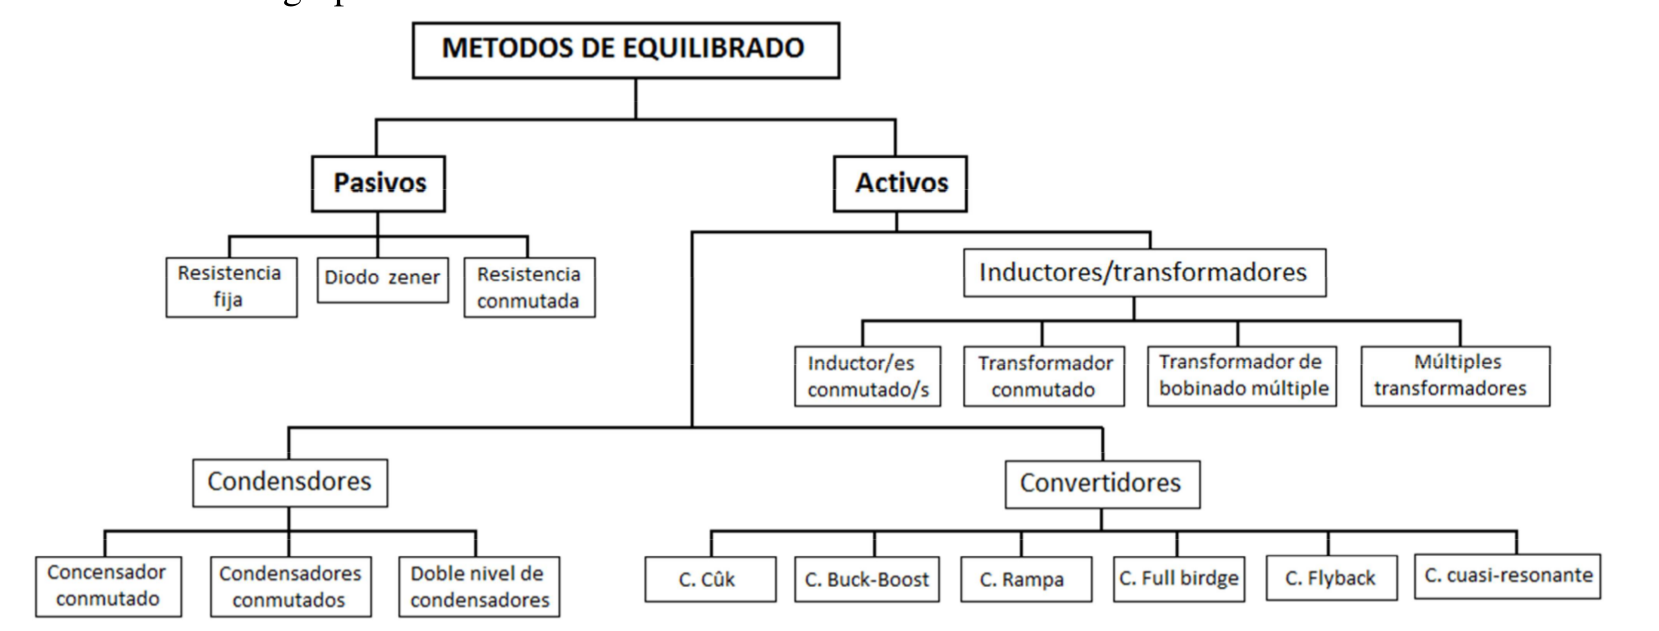
\includegraphics[width=\textwidth, height=12cm] {BMS/metodosequilibrado.png}
    \caption{Mètodes de balanceig de cel·les.}
\end{figure}

\subsection{Causes del desbalanceig de cel·les}
Les principals causes del desbalanceig a les cel·les queden indicades en els següents punts:

\begin{itemize}
    \item Quan es fa el muntatge d'una bateria amb cel·les a diferents nivells de càrrega.
    
    \item Quan es munten cel·les amb el mateix estat de càrrega però diferent historial de cicle. En aquest cas, si bé el sistema d'entrada està balancejat, el desbalanceig començarà a fer-se evident de forma ràpida. El major problema d'aquest desbalanceig es que més enllà de poder-se corregir mitjançant gestions del BMS, tornarà a aparèixer en quan es realitzin cicles ràpids de càrrega i descàrrega. A la pràctica, \newline l'emprar cel·les idèntiques amb diferent ciclat té un efecte similar a posar cel·les amb diferent capacitat. Les cel·les perden capacitat de càrrega/descàrrega conforme són ciclades. Això es per tant un factor que s'ha d'evitar.
    
    \item Per les pròpies diferències entre cel·les producte de toleràncies en la fabricació. Aquestes diferències són causa de petites desviacions de la capacitat real respecte el disseny, de diferents corrents d'auto descàrrega, etc. Aquest és el cas més comú de desbalanceig. Les petites diferències de funcionament entre cel·les es podrà compensar amb l'algorisme de balanceig del BMS de mode que a la pràctica no s'haurien de veure problemes greus de desbalanceig. Com a molt s'ha d'optar per fabricants que garanteixin desviacions petites en el comportament de les cel·les per així eludir part del problema.
    
    \item En molts casos, és el propi BMS el que provoca efectes de desbalanceig. Principalment en bateries amb un nombre de cel·les per sobre de 3, es solen emprar esgraons d'alimentació de mode que grups de cel·les alimenten parts de l'electrònica, i així demanar de forma equivalent a cada cel·La. A la realitat el que succeeix és que hi ha cel·les que contribueixen més a l'alimentació de control que altres i això a llarg plaç podria ser causa d'un desbalanceig de cel·les. El sistema de gestió de balanceig ha de ser capaç de contrarestar aquest efecte, que a més a més, és a molt llarg plaç doncs els consums dels sistemes de gestió śon de molt poca potència.
\end{itemize}

\subsection{Balanceig passiu}
És el balanceig més emprat. Es basa en descarregar la cel·la o cel·les més carregades mitjançant una resistència. Aquesta tècnica empra una \newline resistència per dissipar l'excés de càrrega que pot acumular una cel·la fins que la seva tensió de sortida cau per sota del punt de voltatge de regulació. És per això que també reben el nom de balanceig dissipatiu. Els grans avantatges del mode passiu són el baix cost de components i la simplicitat en el disseny i control. Òbviament, el gran inconvenient és que tota l'energia manejada en el procés de balanceig és una energia perduda.

L'algorisme bàsic es pot fer més complex tenint en compte altres variables de decisió com pot ser la tensió de cel·la o el mode en el que es trobi la bateria. Per un costat, és convenient establir una tensió mínima de cel·la per la qual la gestió de balanceig es desactivi. Això garanteix que en sistemes amb baix estat de càrrega de les cel·les, el balanceig les descarregui encara més.

Una altra configuració habitual és permetre el balanceig només quan la bateria es troba en mode càrrega. Imaginem la bateria amb un estat de càrrega X, i es deixa durant setmanes o mesos sense ús. Si el balanceig actua, pot provocar que l'estat de carrega real al cap de les setmanes sigui molt diferent al que indica la bateria. Per altra banda, en un procés de carrega complert es produeix l'actualització de l'estat de càrrega del sistema, amb el qual no afecta en aquest aspecte el tenir activat el balanceig.

\begin{figure}[H]
	\centering
    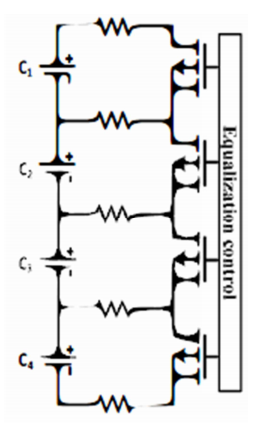
\includegraphics[width=7cm, height=7cm] {BMS/balanceopasivoresistcomutada.png}
    \caption{Balanceig passiu per resistència commutada}
\end{figure}

El dimensionat del circuit de balanceig es basa en decidir el corrent màxim de balanceig. Aquest valor ha de ser un compromís entre diferents aspectes. Per un costat, interessaran corrents alts de mode que un possible desbalanceig sigui corregit el més ràpid possible per part del BMS. Pel contrari, sobredimensionar aquest circuit implica utilitzar transistors mosfets i resistències de major potència, amb el que això suposa un cost de components així com espai per a l'electrònica.

\subsection{Balanceig actiu}
El balanceig actiu de les cel·les d'una bateria està adquirint cada cop més importància ja que soluciona els principals defectes del balanceig passiu. També presenta els seus propis inconvenients, per a un gran nombre de cel·les pot arribar a resultar una cosa antieconòmica. El principal avantatge d'aquest equilibrat és que no dissipa la càrrega que tenen en excés les cel·les sinó que l'utilitza per equilibrar cel·les menys carregades a través de condensadors o inductors aconseguint un ús més eficient de l'energia i un major compte sobre la bateria, el que augmenta la seva vida útil.

Els principals inconvenients d'aquest tipus de balanceig són:
\begin{itemize}
    \item Complexitat i cost de l'electrònica associada al balanceig.
    \item Complicació en la gestió del balanceig.
    \item Sorolls de commutació.
\end{itemize}

El mètode principal en la majoria d'implementacions de BMS amb balanceig actiu es realitza mitjançant una càrrega capacitiva. És a dir, fent servir un condensador.

Aquest mètode es basa en curtcircuitar la cel·la més carregada a un condensador i a continuació buidar aquest sobre la cel·la adjacent més descarregada. Aquest mètode té moltes limitacions.

Per una banda l'electrònica de commutació ha de poder manejar els pics de corrent que es produiran en els processos de càrrega i descàrrega. Les pèrdues d'energia poden estar al voltant del 50\%. Un altre problema és que la capacitat de transferència d'energia és proporcional a la diferència de tensions entre les cel·les de càrrega i descàrrega amb lo que el balanceig serà efectiu només en els extrems dels cicles de càrrega per ser les zones on es donaran les majors diferències de tensió entre cel·les. Aquests pics de corrent a més a més provocaran soroll en l'electrònica de control que ha de ser tingut molt en compte per evitar problemes en les mesures.

El balanceig es farà lent a mesura que hi hagi més cel·les en sèrie. Si es suposa que hi ha 3 cel·les en sèrie, sent la cel·la 1 la més carregada i la cel·la 3 la més descarregada. Idealment el balanceig actiu per càrrega capacitiva hauria de carregar el condensador amb la cel·la 1 i descarregar-ho a la 3, però com no són cel·les adjacents primerament es tindrà que transferir potència de la 2 a la 3 a menor ritme i després de la 1 a la 2. Si ara en comptes d'haver-hi 3 cel·les tenim 30 i volem descarregar la 10 i transferir-la a la 30, caldrà passar per les 18 cel·les intermèdies i per tant, és un procés lent.

\begin{figure}[H]
	\centering
    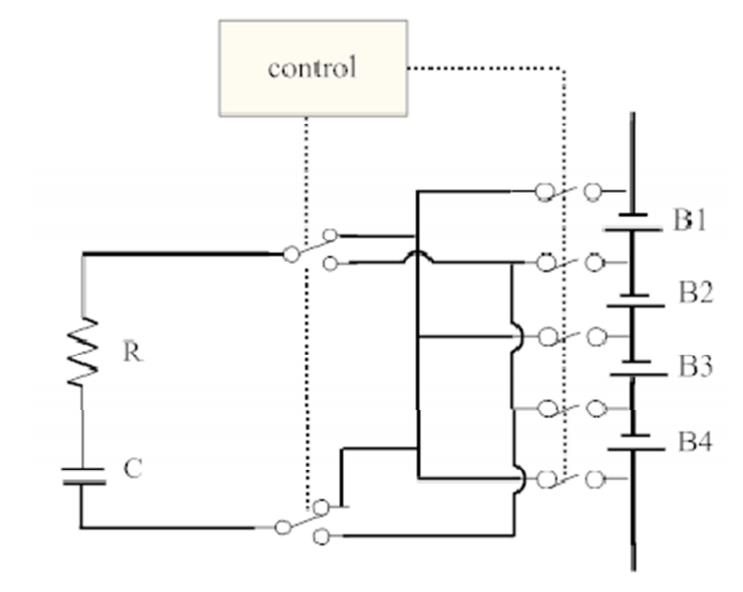
\includegraphics[width=8cm, height=8cm] {BMS/balanceoactivocondensador.png}
    \caption{Balanceig actiu per condensador commutat.}
\end{figure}  

Existeix un segon mètode que està començant a veure's en diferents implementacions del balanceig actiu. Aquest mètode aprofita la càrrega d'una bobina des de la cel·la més carregada per després bolcar l'energia emmagatzemada en aquesta bobina en la cel·la adjacent més descarregada. Millora l'aspecte d'eficiència amb respecte a la càrrega capacitiva principalment pel fet de que els pics de corrent provocats per la topologia capacitiva desapareixen. Això permet a més a més els requeriments en termes de corrent dels components involucrats en el balanceig.

En termes d'eficiència d'operació es pot aconseguir fins a un 90\%. Un altre gran avantatge amb respecte a mode capacitiu és que l'equilibri es pot aconseguir amb independència dels voltatges individuals de les cel·les.

Com aspectes negatius, a més a més d'incrementar els costos i espais dels circuits de balanceig, pot generar problemes de soroll que han de ser tinguts en compte. També, de la mateixa manera que en el cas de balanceig amb càrrega capacitiva, el procés pot alentir-se si hi ha cel·les al mig d'entre les cel·les amb valors de càrrega extrems.

\begin{figure}[H]
	\centering
    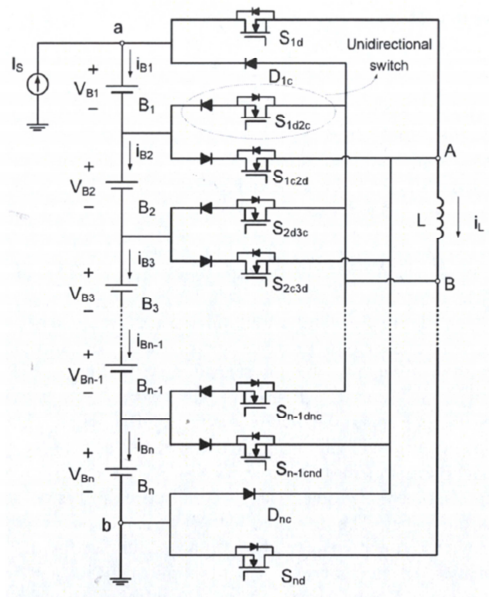
\includegraphics[width=5cm, height=6cm] {BMS/balanceoactivoinductor.png}
    \caption{Balanceig actiu per inductor commutat.}
\end{figure}    


\chapter{Prototip}
\label{chap:Prototip}

%Introducció
El nostre prototip consisteix en un BMS capaç de balancejar cel·les, controlar la temperatura i la càrrega i descàrrega. Aquests són els principals factors que cal controlar d'una bateria. Cal destacar que el BMS és modular, és a dir, que es poden afegir diferents mòduls per augmentar el nombre de cel·les i per tant el voltatge. D'aquesta manera depenent del nombre de cel·les hi hauran més o menys mòduls i per tant el nombre de bateries que pot controlar és més flexible. A més a més el nostre prototip incorpora un control extern del BMS basat en l'integrat d'Atmel (Arduino) de la placa BMS. Pel nostre prototip només s'ha arribat a plantejar la placa BMS mestre, no s'ha tingut en compte els BMS esclaus ja que no s'ha pogut assolir el projecte fins a l'objectiu plantejat a l'inici.

Avui en dia l'electrònica està molt avançada i és per això que no cal \newline necessàriament dissenyar un BMS des de zero, ja que es proveeixen certes parts, les quals faciliten molt la implementació. Aquests mòduls venen en forma d'integrats i pràcticament s'encarreguen de la part més complexe del que seria un BMS en la seva totalitat. És per això que ens hem basat en un d'aquests integrats per tal d'implementar de forma teòrica un prototip de BMS. 

\section{Selecció de l'integrat per al prototip BMS}
En primera instància, al moment d'indagar sobre possibles integrats per al nostre prototip vam veure un xip de la família Atmel que ens va cridar molt l'atenció. Aquest xip era el ATA6870N. La part bona d'aquest integrat és que ja hi havia un projecte a Internet el qual serviria molt bé com a guia. Aquest projecte proporcionava tant el hardware com el software del BMS i facilitava molt la seva implementació real. Quan vam veure que era viable vam escollir aquest integrat per al prototip. Dos mesos després de feina, quan vam començar a pressupostar el prototip, ja que el disseny ja el teníem, ens vam adonar que aquest integrat es va deixar de fabricar feia uns mesos ja que l'empresa Atmel va tancar. Per tal de no fer servir un integrat que estava fóra del mercat es va haver de redirigir tot el projecte amb l'elecció d'un nou integrat. Aquest integrat és el BQ76pl455a-q1. 

Aquest integrat supera en gran mesura la complexitat i abast de l'integrat d'Atmel. Controla més cel·les, té un disseny més elaborat, permet comunicacions aïllades entre mòduls, entre d'altres aplicacions. La part negativa es que no donen un disseny total d'un BMS ni el software. Per tant la implementació real es complica en gran mesura. Per anomenar d'una forma més còmoda aquest integrat li direm BQ.

\begin{figure}[H]
	\centering
    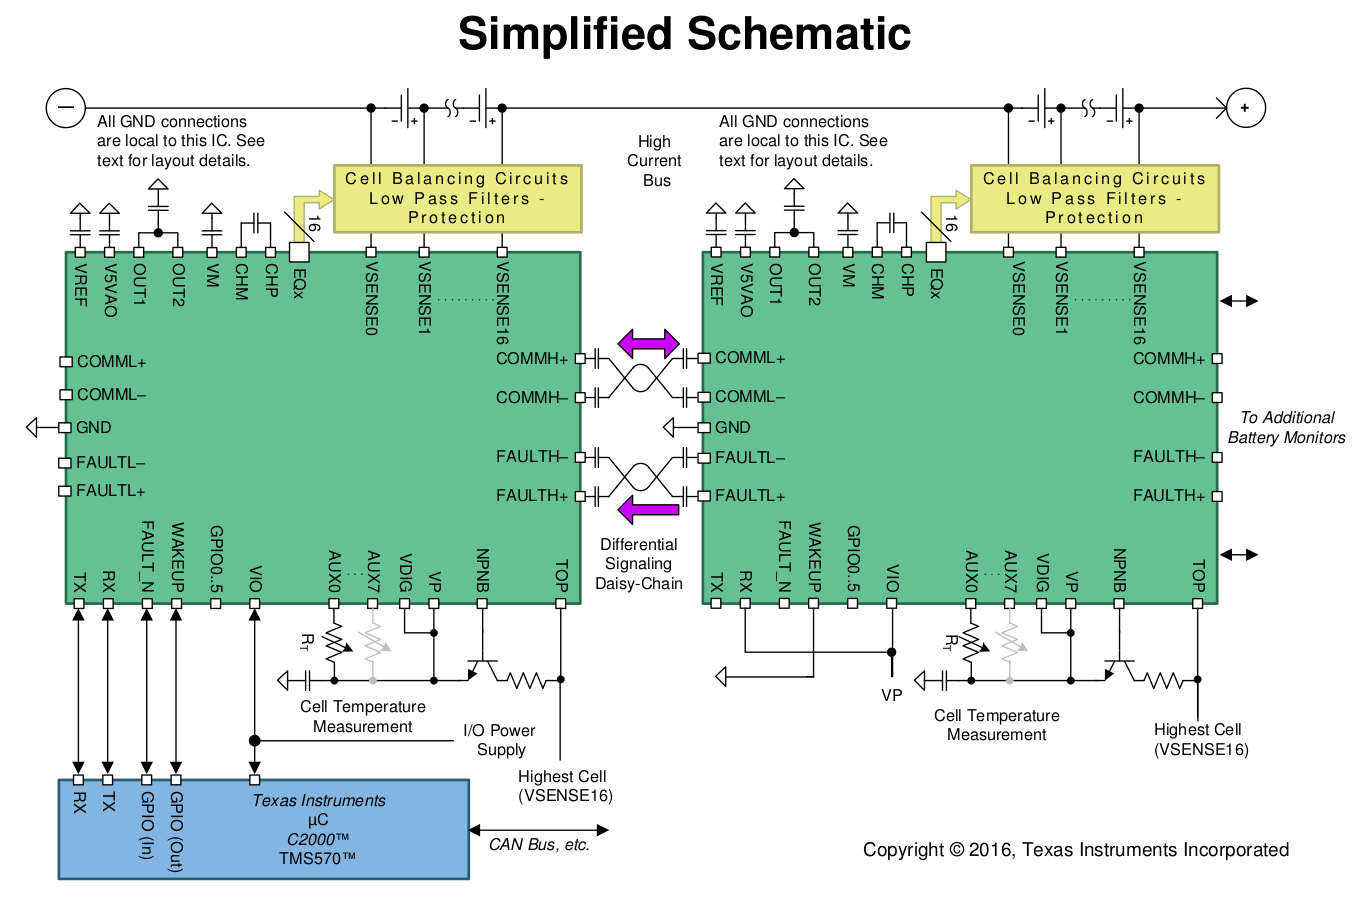
\includegraphics[width=\textwidth, height=10cm] {Prototip/esquematicsimplificat.png}
    \caption{Diagrama simplificat del BQ76pl455a-q1.}
\end{figure}

\section{Coneixent l'integrat BQ76pl455a-q1 }

El BQ és un integrat preparat per a monitorar i protegir fins a 16 cel·les, amb un disseny d'alta confiança per a motors elèctrics. La gran velocitat de l'integrat, la comunicació capacitiva aïllada diferencial i l'alta diversitat de possibles comunicacions ha fet que ens decantéssim per aquest integrat. Lo bo d'aquest integrat es que monitora i detecta un munt de diferents possibles condicions de falla, incloent: sobrevoltatge, sota voltatge, sobre temperatura i falles de comunicació. També té entrades digitals i analògiques per afegir monitoreig addicional i funcionalitats de programació. També incorpora una parada d'emergència en cas de sortir dels rangs de temperatura que s'admeten en una bateria.

Les aplicacions principals d'aquest integrat són per al control de vehicles elèctrics, sistemes de 48V quan només s'utilitza un únic integrat, per emmagatzemament d'energia (UPS) i per a bicicletes elèctriques.

A continuació s'esposarà el funcionament d'aquest integrat per a les diferents funcionalitats que proveeix.

\subsection{Màquina d'estats del BQ}

L'integrat escollit per aquest projecte té molts estats interns que succeeixen en la seva electrònica, però a grans trets estan diferenciat en tres estats: Shutdown, Idle i Wake up. L'estat de Shutdown seria quan la bateria no estigués connectada al BMS i per tant, no estigués rebent corrent el microcontrolador. També podria ser que es forcés una parada des del microcontrolador. És l'estat de parat. L'estat Idle és l'estat de funcionament i és on tot està funcionant, tant el balanceig, el monitoreig, processament de dades... En definitiva, tot el que envolta les funcions d'un BMS. L'estat de Wake up consisteix en el moment en el que el BQ passa d'estar de Shutdown a estat Idle. Es converteix en un estat ja que el seu procés és bastant complexe. De no ser així estaríem parlant de la màquina d'estats més simple que hi pot haver, que funciona o no funciona, encara que el BQ presenta algunes característiques especials quan està en mode Shutdown.

\subsubsection{Estat de funcionament (IDLE state)}
No s'entrarà en detall ja que és quan el BQ no es troba en cap dels altres dos estats. Simplement és quan l'integrat està en funcionament, és a dir, està realitzant la funció de control en un BMS. Sempre i quan surti de la funció de BMS sobre una bateria es trobarà en els altres dos estats. Al llarg d'aquest capítol es parlarà sobretot del funcionament del BQ com a BMS i per tant, estarem parlant tota l'estona de l'IDLE state.

\subsubsection{Estat d'encesa (Wake up state)}
L'estat d'encesa pot ser ocasionat per dos únics factors. En primer lloc l'integrat disposa d'un pin anomenat \textit{WAKEUP} que si es posa en estat alt quan el BQ està apagat el posa en estat d'encesa. Aquest pin només està pensat per a la placa mestre del BMS, la qual estaria connectada a un microcontrolador. El microcontrolador seria l'encarregat de posar en marxa l'integrat posant a nivell alt el pin de \textit{WAKEUP}. Aquest pin només té sentit per als BMS mestres ja que en cas de que hi hagin connectats mòduls esclaus, aquests seran activats mitjançant les comunicacions. 

En el cas en el que hi hagi un BMS mestre i diferents mòduls esclaus en el moment que s'apliqui un senyal que provoqui l'estat d'encesa quan l'integrat està apagat, cal que torni a nivell baix per a que l'integrat pugui tornar a l'estat de parada. En aquest moment, el BQ transmetrà el senyal d'encesa pels seus pins de communicació al següent mòdul esclau, on els pins de communicació el rebran i rebotaran cap al següent mòdul.

El pin de \textit{WAKEUP} usualment es troba a nivell baix. Si aquest pin es posa a nivell alt i l'equip ja havia estat avisat per parar-se, immediatament es tornarà a encendre i posar en estat de funcionament. Per evitar problemes, aquest pin no pot estar mai flotant, sempre cal que estigui definit a nivell alt o baix. Mentre l'integrat es troba en estat apagat els pins de communicació que connecten amb el mòdul adjacent més proper a la placa mestre estan escoltant per a si reben un senyal d'encesa. 

Si el pin de \textit{WAKEUP} es posa a nivell alt quan l'integrat està en l'estat de funcionament es provoca un reset i l'integrat torna a començar per l'estat de Wakeup.

\subsubsection{Estat de parada (Shutdown)}

L'estat de parada és l'estat de potència més baix disponible per al BQ. En aquest estat el BMS talla la potència de la bateria, deshabilita el monitoreig per a la majoria de blocs interns, inclosos els de control. Típicament, l'estat de parada són per a períodes llargs d'inactivitat quan la bateria no estigui sent carregada o descarregada. La part que ha de rebre el senyal per a que el BMS es posi en funcionament és a través del pin de \textit{WAKEUP} o per les comunicacions entre plaques mestre i esclau, ja que les comunicacions es queden en mode d'escolta en l'estat de parada. 

Per entrar en l'estat de parada, s'ha de deixar d'alimentar els pins que alimenten l'integrat; el VP i el VDIG. El pin VIO pot romandre alimentat en l'estat de parada. Els pins VP i VDIG han d'estar totalment desconnectats ja que sinó provocarien una potència negativa. El pin de \textit{WAKEUP} ha d'estar en tot moment a nivell baix per a què no tregui a l'integrat de l'estat de parada. 

Totes les condicions que poden provocar un estat de parada queden resumides en els següents punts:

\begin{itemize}
    \item A través del microcontrolador s'envia un ordre de \textit{SHUTDOWN}.
    \item Timeout ocasionat a les comunicacions.
    \item El voltatge VDIG té valors inferiors al seu llindar mínim.
    \item Un dels sensors interns de temperatura detecta un valor fora dels llindars.
    \item Detecció de falla en els controls de l'integrat.
\end{itemize}

En el nostre cas com que tot el disseny estarà implementat en una mateixa placa, i el pistejat d'aquesta serà fixa, no podrem aprofitar l'ús del VIO en el nostre BMS per alimentar al microcontrolador, ja que s'alimenta de la pròpia bateria que en estat de SHUTDOWN el microcontrolador la talla. 

\subsection{Voltatges de funcionament del BQ}

El BQ té la peculiaritat de que s'alimenta fent ús de la pròpia bateria que gestiona, si les cel·les no estan connectades el microcontrolador no funciona. Un integrat sol treballar a voltatges petits d'un valor d'entre 5 i 7 volts per norma general. Si s'alimenta de la pròpia bateria estem parlant de fins a valors d'uns 60V. Cal d'una electrònica externa per tal de convertir aquests 60V en un voltatge òptim per al microcontrolador. 

\begin{figure}[H]
	\centering
    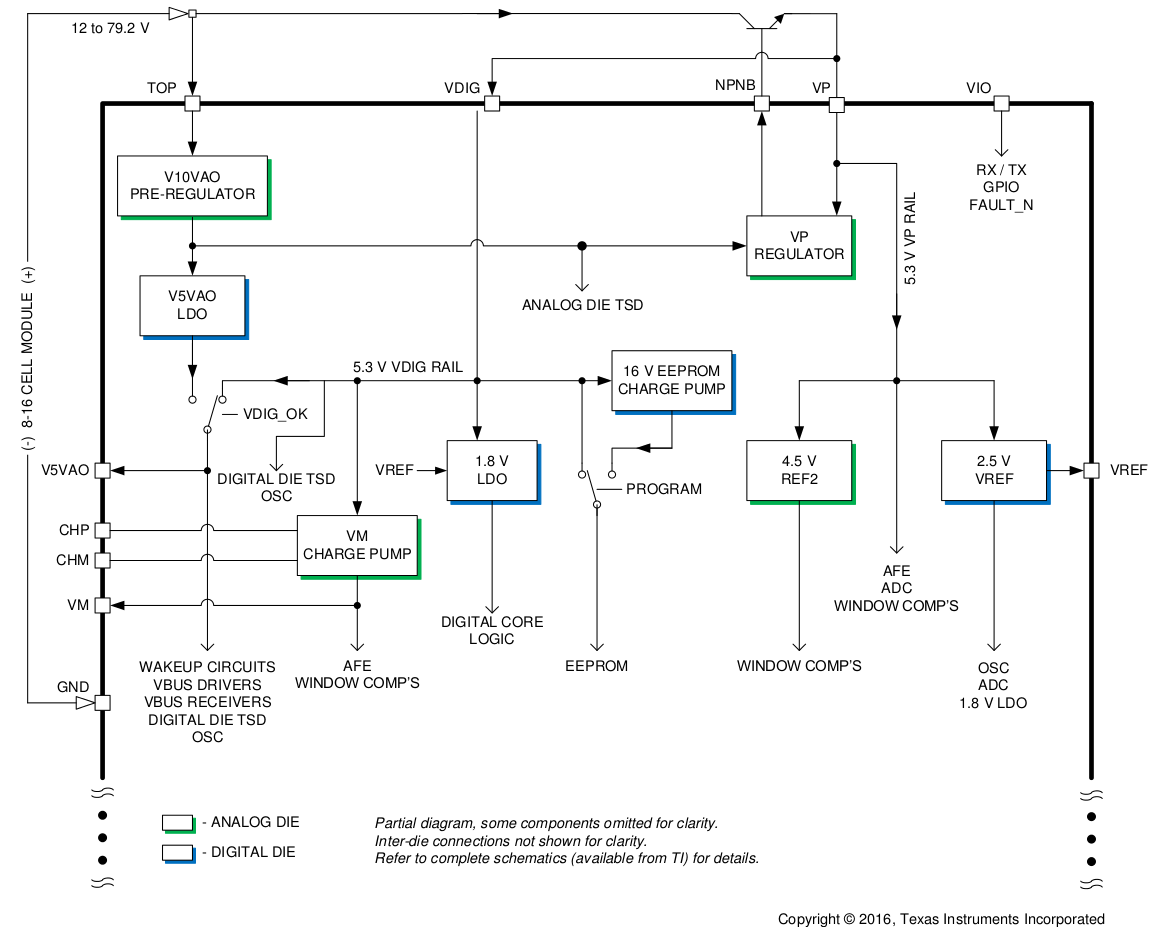
\includegraphics[width=\textwidth, height=10cm] {Prototip/diagramavoltaje.png}
    \caption{Diagrama complert de voltatge.}
\end{figure}

\subsubsection{Alimentació de l'integrat (VP i TOP)}
Com s'acaba de comentar els integrats treballen a uns valors electrònics molt inferiors al voltatge de la bateria que s'està tractant en aquest prototip. Els límits de l'alimentació d'entrada es troben entre -0.3 i 5.5V. Cal reduir doncs aquest voltatge elevat en uns valors vàlids per a l'integrat. El pin d'entrada d'alimentació és el VP. 

Per a tractar aquest voltatge el fabricant recomana l'ús d'un transistor NPN de potència per generar una nominal de 5.3V, que és el voltatge de funcionament òptim per a l'integrat. El tret del transistor es realitza internament mitjançant el pin NPNB. En el moment que la bateria es connecta, internament el pin NPNB s'activa i dispara el transistor per alimentar l'integrat. Quan arriba el senyal al transistor ja ve filtrat per dos filtres pas-baix per tal de reduir al màxim el soroll. És molt important controlar el corrent en aquest punt ja que la potència ve directa de les cel·les on està connectada. El corrent és de de la cel·la més alta fins a la cel·la més baixa del muntatge de cel·les. La cel·la més alta de la bateria es connecta també al pin TOP. Aquesta connexió es realitza amb un filtre pas-baix per evitar efectes de soroll, ja que les bateries en generen molt. El filtre pas-baix sol tenir una constant de temps similar a les entrades VSENSE.

El pin TOP també s'utilitza per a l'alimentació de l'integrat i com a mesura total de la bateria, un cop filtrat el senyal. Aquesta mesura és la que indica per medi del hardware l'activació del pin NPNB.

\subsubsection{Alimentació interna de l'integrat (VIO i VDIG)}
Del col·lector del transistor NPN de potència emprat per a l'alimentació de l'integrat, també se n'aprofita una part el pin VIO. Aquest pin s'encarrega d'alimentar la part de l'integrat encarregada de les comunicacions amb un microcontrolador. En concret dóna l'alimentació als pins de GPIO, als de communicació Serial (RX/TX) i al pin FAULTN. A més es pot emprar directament el voltatge de sortida del pin VIO per alimentar un microcontrolador. S'emprarà aquesta tècnica per alimentar el micro del nostre prototip i aprofitar ja els 5V filtrats que ens proporciona. Aquest pin pot no estar connectat, encara que es recomana en tots els casos que ho estigui, ja que cal d'un control extern que gestioni el BMS. 

A més a més no només s'aprofita una part del voltatge que entra a VP per a VIO, sinó que al disseny entra un tercer pin que és el VDIG. Aquest pin és l'encarregat de gestionar el voltatge per als components interns de l'integrat encarregats de realitzar els càlculs. Estem parlant dels ADCs que s'impliquen en els càlculs i lectures dels senyals per al correcte funcionament del BMS. El voltatge entrant per VDIG és regulat fins a 1.8 volts, voltatge al qual treballen els ADCs. El pin VDIG ha d'estar alimentat per a que l'integrat funcioni.

\begin{figure}[H]
	\centering
    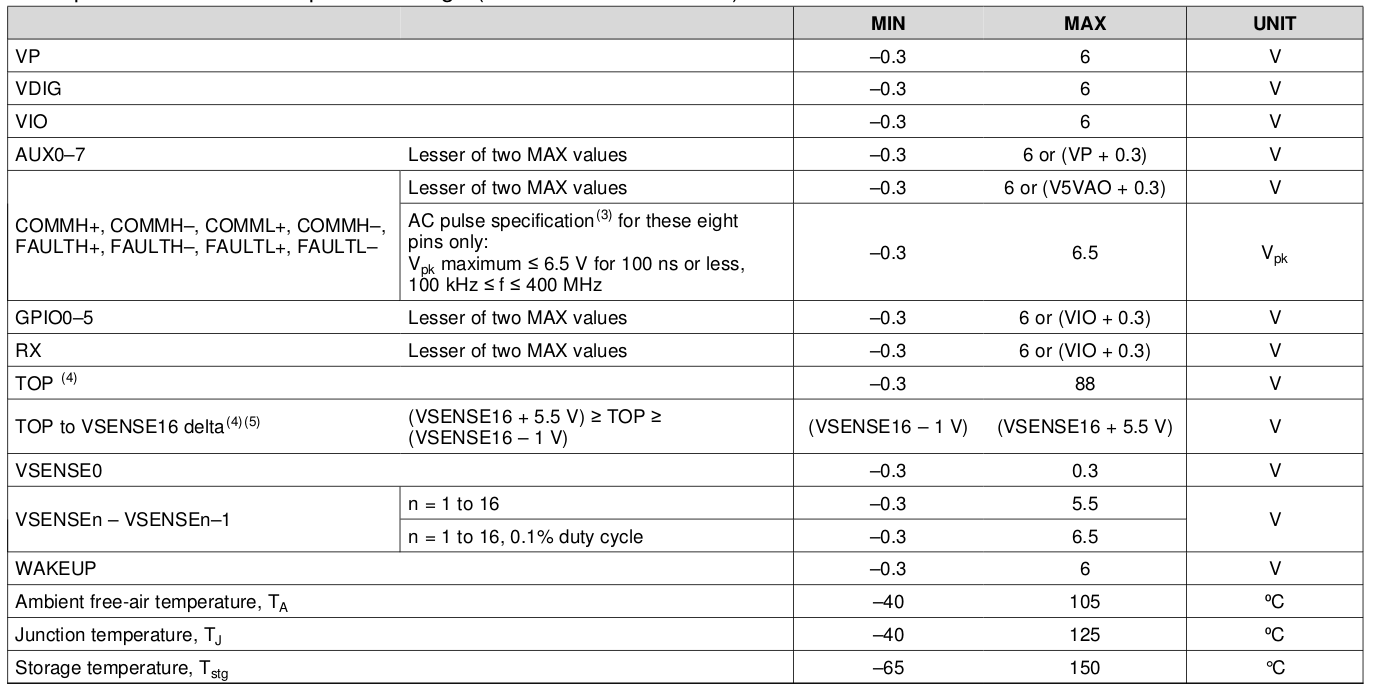
\includegraphics[width=\textwidth, height=8cm] {Prototip/nivelesvoltaje.png}
    \caption{Voltatges de funcionament del BQ76pl455a-q1.}
\end{figure}

\subsection{Balanceig de les cel·les}

Com s'ha anat comentant al llarg del projecte, el balanceig de cel·les és una de les tasques més importants que ha d'implementar un BMS. En termes simples ha de poder mesurar els voltatges de la cel·les i aplicar l'acció pertinent per a que estiguin balancejades en tot moment. Les lectures de les cel·les del nostre prototip es realitzen mitjançant el pin VSENSE (pin on es connecta el pol positiu d'una cel·la), aquest pint té un rang entre 1V i 4,95V. Aquesta lectura indica al microcontrolador el voltatge de cada cel·la i depenent d'aquest, part d'aquest voltatge que està circulant per la cel·la es dissiparà a través del pin EQ i el circuit de dissipació associat per tal d'igualar les capacitats de totes les cel·les. Cal afegir que un cop el voltatge entra al microcontrolador primerament és comparat en uns operacionals que ja per hardware indiquen si s'està detectant un sobrevoltatge o un sotavoltatge. En el moment que un d'aquests operacionals detecta un sobre o sotavoltatge, el microcontrolador ho processa detectant un estat de FAULT, pausant el sistema per evitar riscs sobre altres cel·les o el propi microcontrolador i avisant al microcontrolador d'un estat de FAULT. 
L'adquisició dels valors de voltatge de les cel·les es realitzen en el AFE (Analog Front End). El front-end és doncs on es monitoren fins a 16 cel·les. La programació del BQ es pot configurar per tal que monitori tot, un grup, o les cel·les connectades. El mostreig comença des de la cel·la més alta seleccionada i acaba amb la més baixa seleccionada. Durant la mesura, l'AFE tria la cel·la adreçada per un bloc lògic i el canvi de nivell del voltatge de cel·la detectant un guany d'1 fins el pin OUT1 referenciat a terra. La sortida analògica de l'AFE es connecta a OUT1 a través d'una resistència interna. Externament es connecta al pin OUT2 que és on està connectat l'ADC. Això es fa per aïllar internament la part que gestiona les cel·les amb la part que realitza els càlculs, evitant qualsevol tipus de soroll. En aquesta connexió externa entre l'AFE i l'ADC, el requeriment és posar un filtre RC extern per reduir el soroll a l'ample de banda.

 El BQ proporciona tant balanceig actiu com balanceig passiu, encara que és necessita un petit mòdul addicional per aplicar el balanceig actiu. A més a més el microcontrolador permet el balanceig passiu amb una connexió directa. També és la solució econòmica i per tant tots aquests factors han fet escollir aquest tipus de balanceig. 
 
 El balanceig passiu consisteix en dissipar energia a través de resistències de potències, les quals retenen part del corrent i ho transformen en energia calorífica. Cal tenir en compte quina és la potència que es vol dissipar per tal de fer servir una resistència o un altra. En el nostre cas la dissipació externa podrà ser de fins a 1W. El propi microcontrolador ja porta a l'entrada dels diferents VSENSEn una resistència que ja fa una primera limitació de voltatge.
 
 El BQ implementa doncs el balanceig de les cel·les a través dels pins de EQ1..EQ16. S'utilitzen 16 drivers de control, els quals el fabricant no explica el seu funcionament. Les configuracions de funcions disponibles del balanceig són de l'estil de comandes ON o OFF o específiques per a córrer en un temps específic. L'integrat també disposa d'un registre que habilita o deshabilita el balanceig. Aquest registre pot ser modificat per nosaltres per tal d'activar o desactivar el balanceig. Quan succeeix un problema aquest registre s'automodifica parant el balanceig i evitant possibles errors al BMS. A més l'integrat s'apodera de la sortida EQ de la cel·la i el connecta internament al VSENSE de la cel·la inferior reduint el balanceig de corrent a 0.

\subsection{Control de la temperatura}

La forma en la que aquest integrat controla la temperatura és molt bona. Disposa per defecte un sistema de control de temperatura intern, composat per dos sensors de temperatura connectats directament als ADCs, un per la zona de l'integrat que tracta les cel·les i l'altre per a la pròpia electrònica de control de l'integrat. Aquests sensors mostren la temperatura de forma automàtica al control, el control després té en compte aquests valors per si ha de forçar una parada o reduir el voltatge de les cel·les. El propi integrat ja porta incorporada una protecció per defecte molt bona, ja que es troben a dins de l'integrat. Aquests sensors estan totalment implementats pel fabricant i no cal de cap mena de configuració ja que es basen en les temperatures de funcionament dels components de l'integrat. 

\begin{figure}[H]
	\centering
    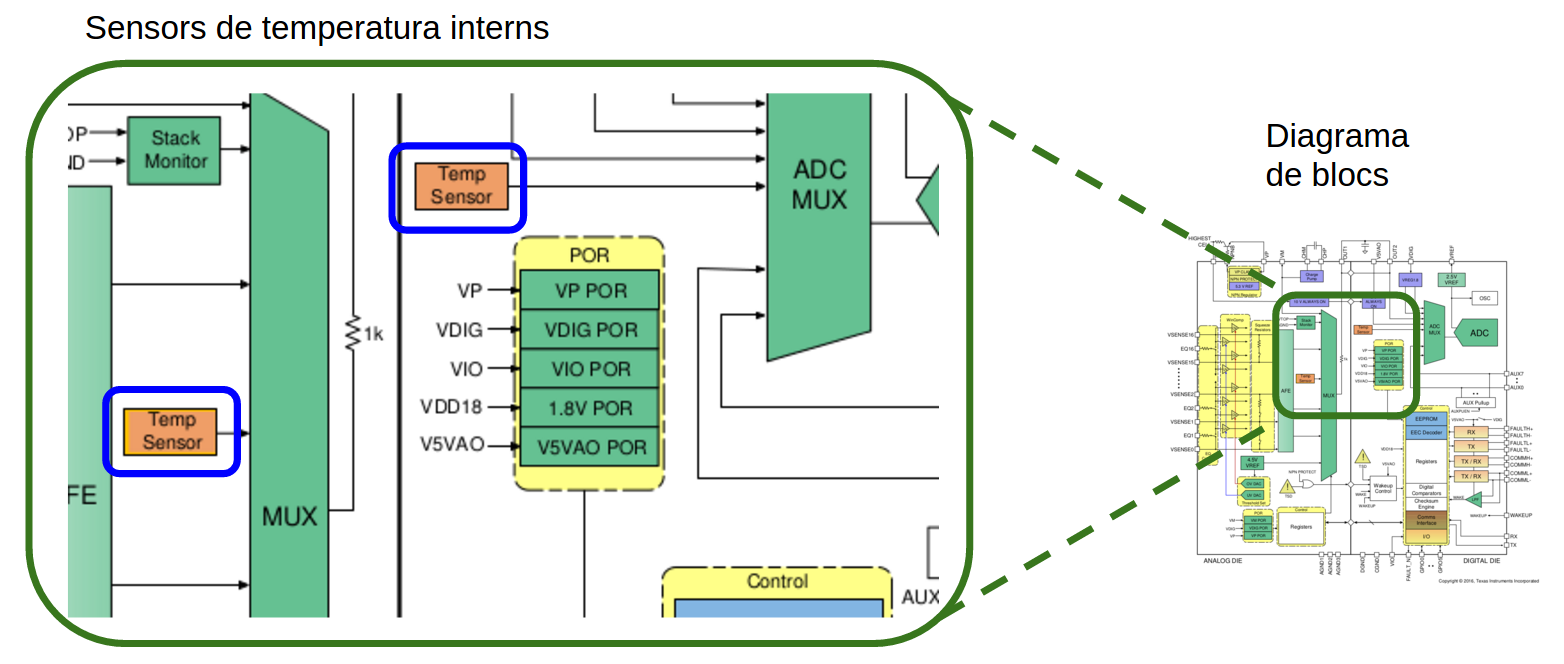
\includegraphics[width=\textwidth, height=7cm] {Prototip/sensorestemperaturainternos.png}
    \caption{Sensors de temperatura interns del BQ76pl455a-q1.}
\end{figure}

A part, el BQ disposa de fins a 8 entrades analògiques de 14 bits (AUX0..AUX7), amb un rang de 0 a 3V per a AUX0 i AUX1, i un rang de 0 a 5V per a la resta d'entrades. Aquests sensors es poden acotar mitjançant uns registres llindars, els quals permeten afinar molt més els rangs. L'ús més comú per aquestes entrades és mitjançant l'ús de termistors. Un termistor és un sensor de temperatura per resistència. El seu funcionament es basa en la variació de la resistivitat que presenta un semiconductor amb la temperatura. Bàsicament es pot mesurar la temperatura a través de termistors.

L'integrat per sí mateix, no té cap mena de control sobre aquests pins AUXn, és a dir que no és capaç de processar les temperatures mostrades per aquests. L'únic que realitza el control és l'enviament d'aquests valors a un microcontrolador. És el microcontrolador qui ha de processar les dades i donar ordre sobre el control. Per defecte, quan s'inicialitza l'integrat comença un comptador cada 1 segon que mostreja els sensors de temperatura, temps més que suficient per a veure l'estat d'una cel·la, ja que no varien tan ràpidament com veure la diferència en 1 segon. 

\subsection{Comunicació entre mòduls BQ}

Per aplicacions on es requereixi múltiples mòduls BQ (un mestre i la resta esclaus), l'integrat proveeix d'un bus de comunicació diferencial que permet al mòdul mestre controlar fins a 16 dispositius, únicament utilitzant una interfície UART. La connexió es realitza en forma de cadena, és a dir, si el mestre és el mòdul 1, els següents mòduls aniran connectats al mòdul adjacent n+1. 

En la configuració en pila, el procés normal de comunicació vindria a ser el següent: 
Primerament el microcontrolador envia una comanda mitjançant el Serial de l'integrat. Un cop el BQ mestre rep les dades, el control genera una communicació que és enviada a través dels diferents mòduls esclau emprant un protocol diferencial de comunicació privatiu del fabricant a través dels pins COMMH+/- i COMML+/-.

Cada equip de la cadena amortigua el senyal. El senyal no es sincronitza o es filtra, passa a través de la cadena i tots els mòduls veuen tota la informació del bus independentment de l'integrat objectiu del senyal. Els paquets arriben a l'ADC de cada un dels integrats i valida el paquet mirant l'adreça objectiu, el contingut del missatge i el CRC. 

\begin{figure}[H]
	\centering
    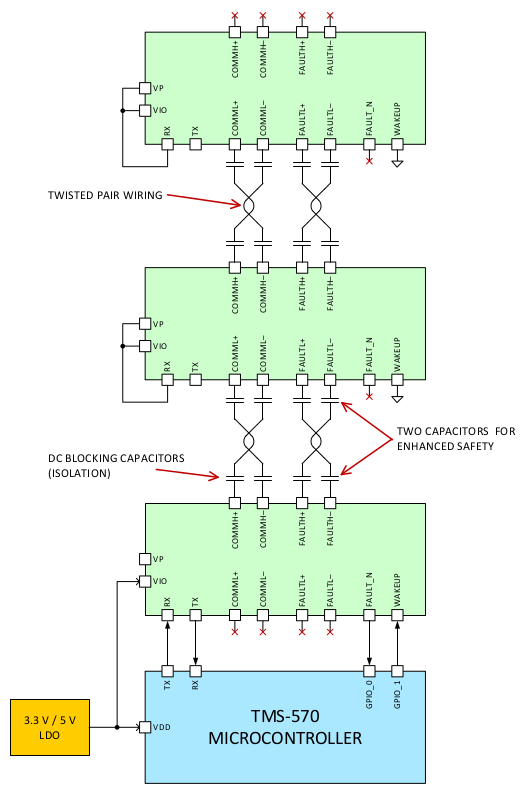
\includegraphics[width=10cm, height=16cm] {Prototip/diagramacomunicacion.png}
    \caption{Connexió entre mòduls BQ76pl455a-q1.}
\end{figure}

\newpage 

En funció del disseny del BMS la communicació entre plaques necessita un disseny o un altre. En el cas que més d'un integrat es trobi en la mateixa PCB no cal un aïllament per a les comunicacions. En canvi, si es troben en PCBs diferents, és obligatori fer ús de components d'aïllament. Quan estan a la mateixa PCB, aquest seria el disseny recomanat pel fabricant:

\begin{figure}[H]
	\centering
    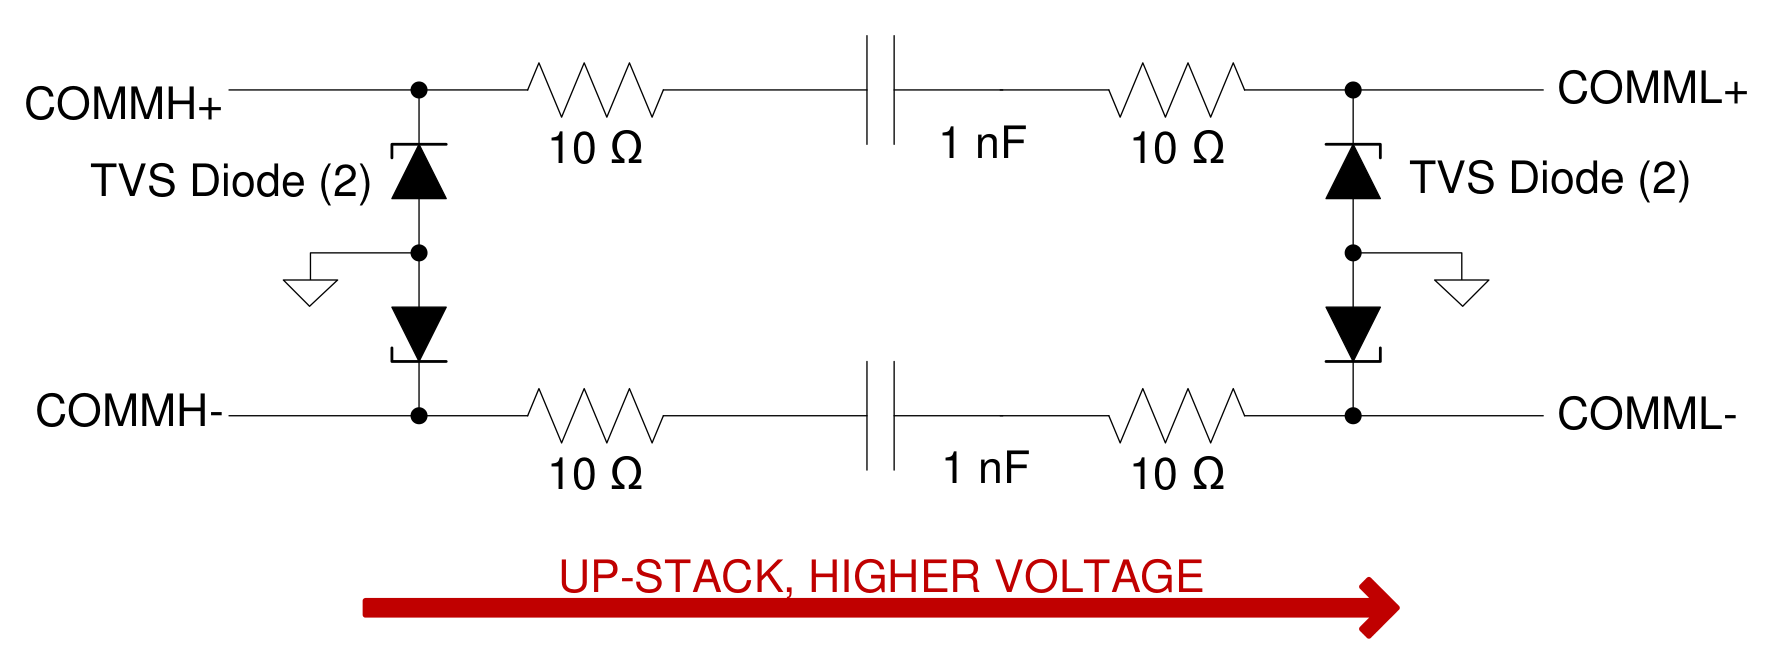
\includegraphics[width=12cm, height=5cm] {Prototip/esquemasamepcb.png}
    \caption{Circuit de connexió entre mòduls BQ a la mateixa PCB.}
\end{figure}

En canvi si els mòduls es troben allotjats en diferents PCBs, el disseny que s'empraria seria el següent:

\begin{figure}[H]
	\centering
    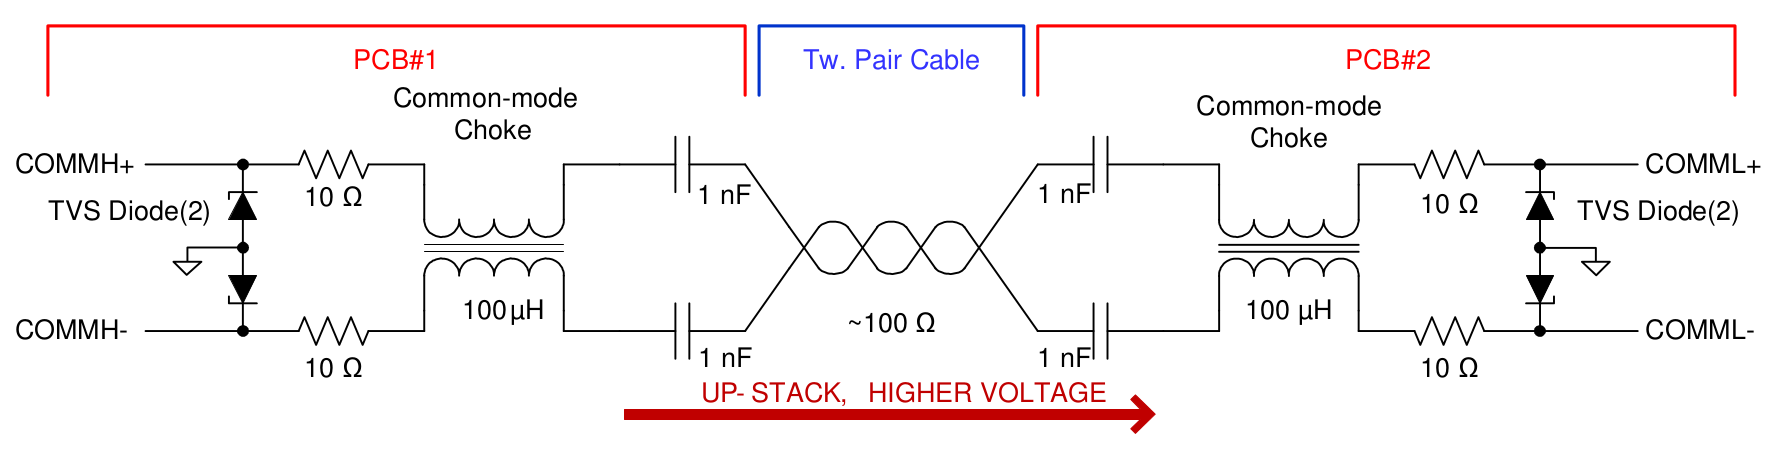
\includegraphics[width=12cm, height=5cm] {Prototip/esquemadifpcb.png}
    \caption{Circuit de connexió entre mòduls BQ en diferents PCB.}
\end{figure}

En el nostre cas ens hem basat en el segon disseny, ja que només tenim pensat posar un mòdul per PCB, on cada un d'aquests integrats controlaria fins a 16 cel·les. En aquest segon disseny l'aïllament es  realitza mitjançant un transformador i condensadors i resistències per a controlar el senyal.

\subsection{Comunicació serial amb el microcontrolador}

El protocol que empra aquest integrat per a la communicació el realitza mitjançant l'UART. Aquest mètode disposa de dos pins de comunicació, un per rebre (RX) i l'altre per enviar (TX). A través d'aquests pins serà per on el microcontrolador enviarà les ordres per a configurar l'integrat d'una manera concreta. 

\subsubsection{UART}
L'UART segueix el protocol estàndard serial 8-N-1, on s'envia la informació com: un bit de START, seguit dels 8 bits d'informació que es necessiten i terminant amb un bit de STOP. La data rebuda per l'integrat està sobre mostrejada per 16 cops per millorar la fiabilitat de la comunicació.

L'integrat permet que es configurin les comunicacions per a esperar un cert temps després de que s'hagi enviat l'últim bit de recepció per començar a transmetre. El protocol és half-duplex. Això vol dir que només pot estar realitzant-se una acció (entre enviar o rebre) a la vegada. Si està enviant dades pel pin TX ignora totalment el pin RX. Per evitar col·lisions és important que el microcontrolador de control estigui correctament programat i esperi a rebre totes les dades enviades per l'integrat. D'haver-hi alguna col·lisió i les comunicacions deixessin de funcionar el microcontrolador hauria d'enviar un reset de la comunicació. El baud rate del canal de comunicacions del BQ permet rangs que arriben al voltant d'1M. L'integrat també permet controlar uns registres que permeten marcar dos temps de timeout si no arriba cap paquet vàlid.  

\subsubsection{GPIO}
Hi ha 6 pins de GPIO al BQ. Poden ser programats com a entrades o com a sortides. Cada GPIO posseeix una resistència interna de pull-up o pull-down per mantenir el pin en tot moment en un estat conegut. Mitjançant la configuració de registres aquests pins es configuren per a ser connectats a la resistència de pull-up o la de pull-down. 

El pin de GPIO permet també enviar un senyal de FAULT. Normalment aquesta acció es realitzada pel pin de FAULTN, però es pot programar per a que els pins de GPIO també l'enviïn. 

\subsubsection{FAULTN}
El pin FAULTN està pensat per a enviar al microcontrolador un estat de fallida per part de l'integrat. En el moment que l'integrat detecta un signe de FAULT, aquest l'envia en forma de pols pel pin FAULTN per avisar al microcontrolador. 

\subsubsection{WAKEUP}
El pin de WAKEUP s'utilitza per encendre el BMS des del microcontrolador. Per a encendre aquest integrat és necessari que aquest pin rebi un senyal de 5V.  A més a més, si l'integrat ja es troba en estat IDLE i el pin de WAKEUP és posa a nivell alt, l'integrat realitzarà un reset.

\subsection{Atmega2560 com a microcontrolador de control}
El prototip es controlarà mitjançant l'integrat de l'Arduino Mega 2560. Donat que aquest tipus de tecnologia s'ha donat al llarg de la carrera, és molt més fàcil d'implementar i programar que no pas un integrat que no coneixem pas. La idea d'aquest control resideix en el fet de que primerament aquest prototip necessitarà d'un seguit de tests els quals validaran el seu funcionament. El fet de tenir un microcontrolador programable ja a la PCB del BMS suposa l'aplicació directe d'aquest, és a dir, cada cop que es vulguin fer canvis en paràmetres el microcontrolador podrà fer-ho directament. A més, com ja s'ha comentat al llarg del projecte, la implementació del BMS ha estat molt més complicada del que primerament ens semblava. És per això que els esquemàtics encara necessiten retocs per tal d'afegir per exemple vies les quals ens serveixin futurament per testejar el BMS. Per la nostra part el que s'ha volgut fer és únicament la implementació del que seria la circuiteria real del BMS. 

\subsection{Diagrama de blocs i disseny exterior}

\subsubsection{Diagrama de blocs}
\begin{figure}[H]
	\centering
    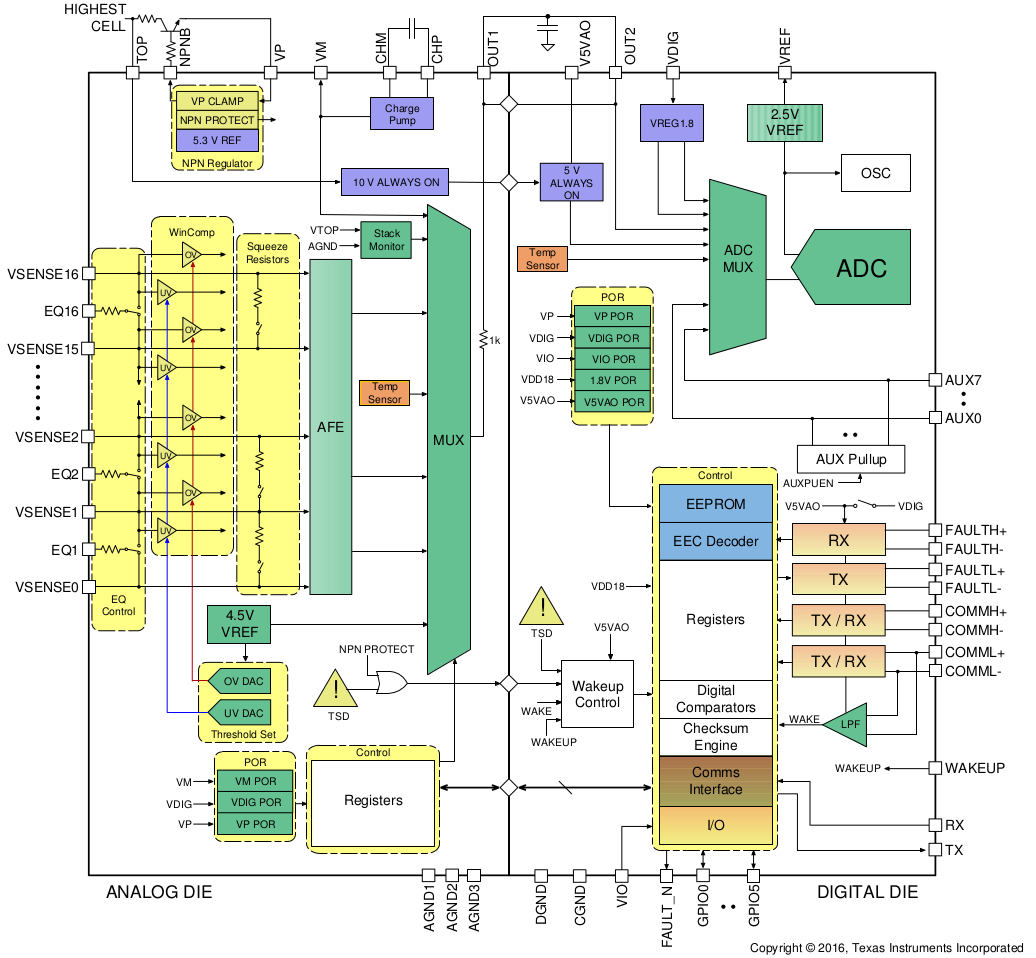
\includegraphics[width=\textwidth, height=14cm] {Prototip/diagramablocs.png}
    \caption{Diagrama de blocs del BQ76pl455a-q1}
\end{figure}

\subsubsection{Disseny exterior}
\begin{figure}[H]
	\centering
    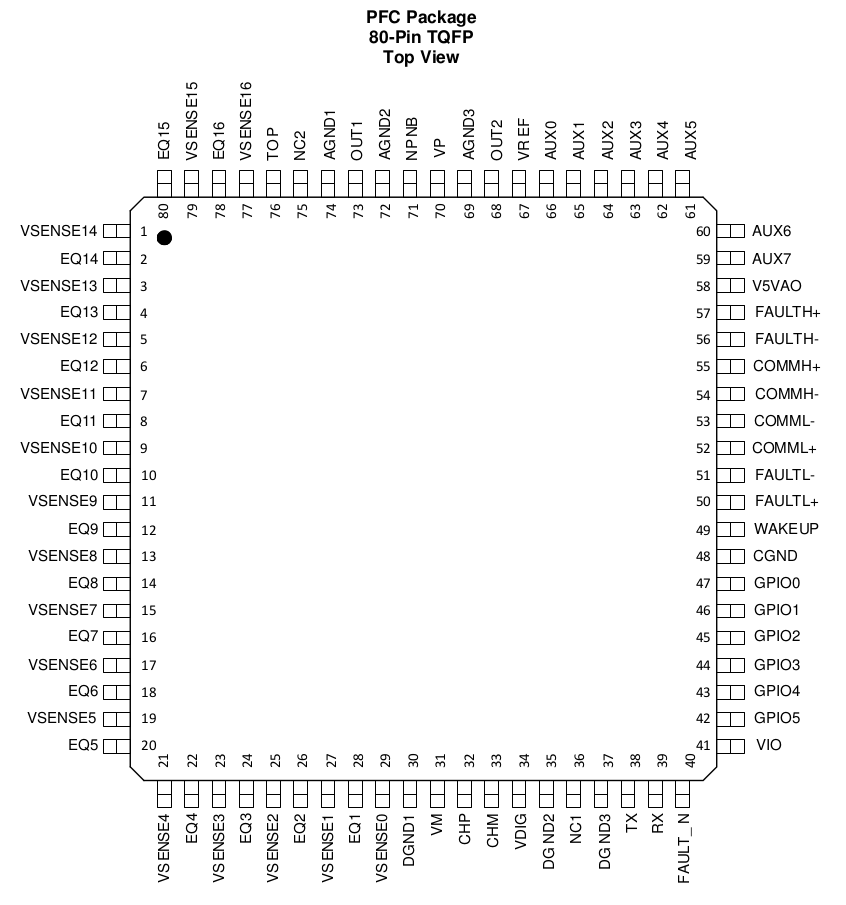
\includegraphics[width=\textwidth, height=14cm] {Prototip/layout.png}
    \caption{Disseny exterior i pins del BQ76pl455a-q1}
\end{figure}

\section{Esquemàtics}

En aquest apartat es mostrarà de forma desglossada els esquemàtics que implementen de forma teòrica el BMS basat en l'integrat BQ76pl455a-q1.

\subsection{Alimentació de l'integrat}
En primer lloc l'alimentació del BQ es realitza per medi del propi corrent de les bateries. Aquest integrat funciona a un rang de 5V mentre que la bateria funciona a uns 60V. L'esquema que es mostra a la figura indica el seu disseny per a passar aquests 60V als 5V. 

\begin{figure}[H]
	\centering
    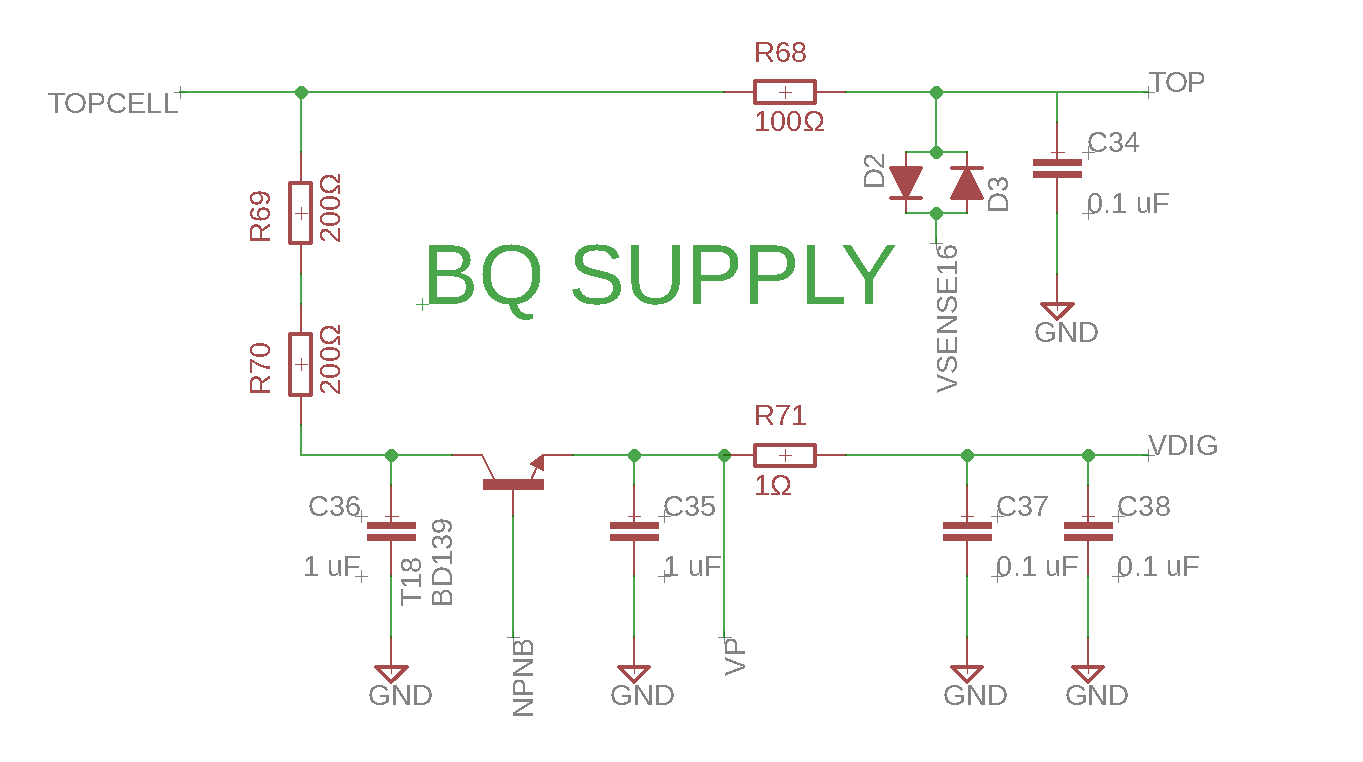
\includegraphics[width=\textwidth, height=8cm] {Prototip/schsupply.png}
    \caption{Alimentació de l'integrat BQ76pl455a-q1.}
\end{figure}

Primerament l'entrada que ve de la bateria ja té un filtrat del soroll \newline mitjançant el doble díode invertit i un filtre RC. Aquí ja el voltatge entra al microcontrolador pel pin TOP. La funció principal d'aquest pin consisteix en fer la lectura total de la bateria. El corrent és novament filtrat fins que arriba al transistor NPNB. Aquest transistor força que l'entrada d'alimentació al pin VP es realitzi a un voltatge de 5V. El col·lector del transistor porta conjuntament amb ell un condensador per evitar canvis bruscs de voltatge. El senyal és novament filtrat i ja entra al pin d'alimentació principal del BQ. El pin VP. A més el senyal és novament filtrat per arribar al pin d'alimentació VDIG, el qual s'encarrega d'alimentar tota la circuiteria dels conversors analògic-digital que incorpora el BQ. D'aquesta manera s'assegura que arriben voltatges de 5V totalment filtrats per evitar tots els problemes que suposa el soroll al corrent.

\subsection{Anivellació de cel·les}

En la següent figura es mostrarà com s'ha implementat l'anivellació de cel·les. Aquí ens hem basat totalment en les especificacions del fabricant ja que es desconeix com l'integrat realitza els algorismes de balanceig. Per VSENSEn entrarà el positiu de la bateria a l'integrat, on és recollirà el voltatge analitzat per l'AFE i enviat al control. El control enviarà aquesta energia a dissipar pel pin EQn. 

Cal destacar que el negatiu de les bateries és diferent al negatiu de tot el BMS, encara que el negatiu també es connecti al BMS.

\begin{figure}[H]
	\centering
    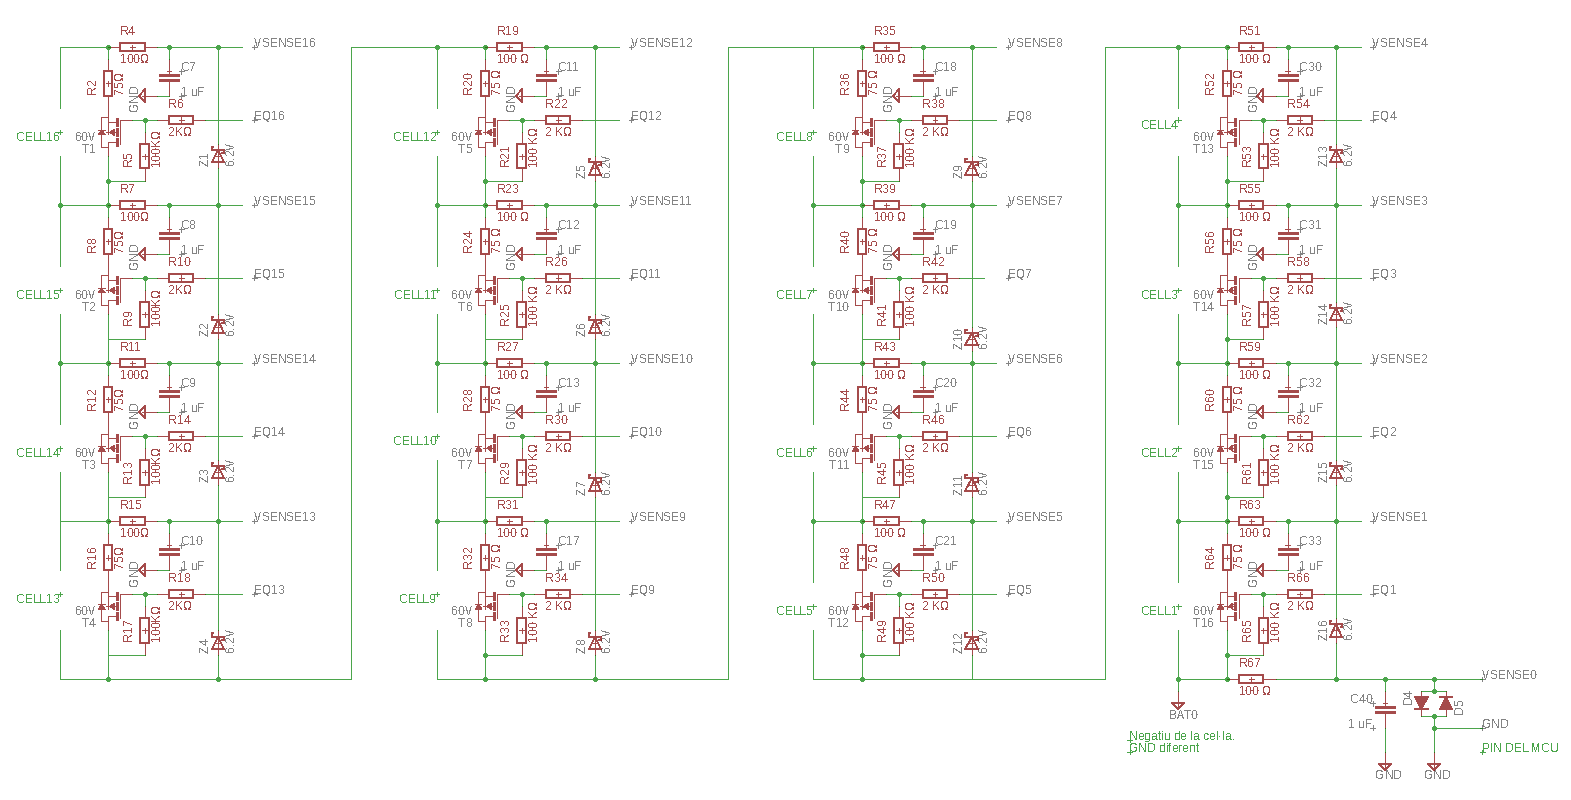
\includegraphics[width=\textwidth, height=10cm] {Prototip/schbalancing.png}
    \caption{Circuit de balanceig de les cel·les}
\end{figure}

\subsection{Tractament de la temperatura}
Encara que l'integrat de per sí ja porta sensors de temperatura interns, el fet de disposar d'entrades analògiques per a mesurar el voltatge ha fet que no les puguem deixar passar. La temperatura es calcula amb un termistor, que és una resistència variable la qual varia en funció de la temperatura. La temperatura és mesurada de forma diferencial per parelles. Fins a 4 mòduls de temperatura poden estar connectats a l'integrat, ja que l'integrat disposa de 8 entrades analògiques, les quals van per parelles. Aquestes entrades són gestionades per l'integrat, però en cap moment en processen la seva informació, solament envien la informació al micro el qual serà l'encarregat de processar aquestes temperatures.

A més el senyal és filtrat mitjançant un filtre RC per a que el senyal entri lo més net possible i no provoqui alteracions, encara que amb la mesura diferencial ja es tenen en compte.

\begin{figure}[H]
	\centering
    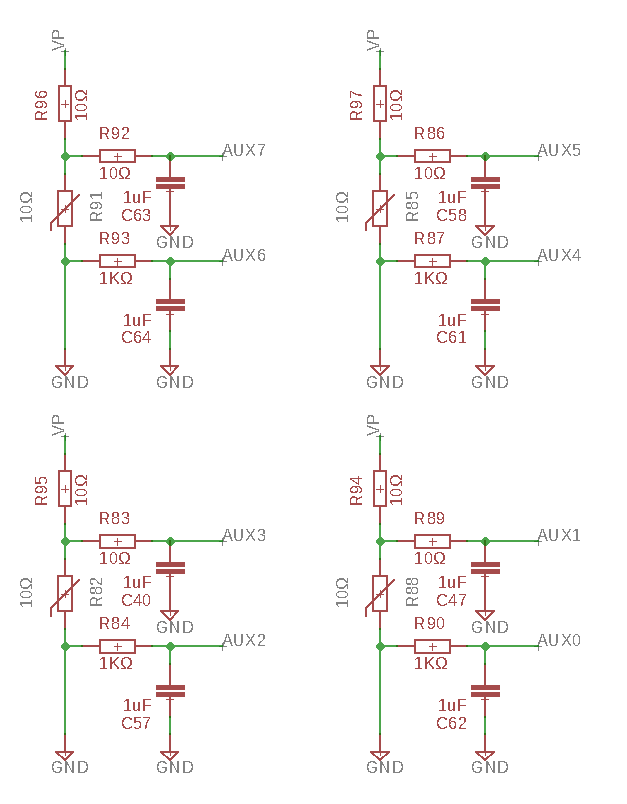
\includegraphics[width=\textwidth, height=14cm] {Prototip/schtemperatura.png}
    \caption{Mesurament extern de la temperatura.}
\end{figure}


\subsection{Comunicació entre Mestre/Esclau}

Depenent de si estem parlant d'un mòdul mestre o un mòdul esclau, aquest esquemàtic pot variar. En el cas de que sigui la placa mestre, les connexions cap a un mòdul n-1 no tenen cap mena de sentit ja que la placa mestre és la placa 1. Això vol dir que només necessita de la part de l'esquemàtic que es connecta a la següent placa BMS.

\begin{figure}[H]
	\centering
    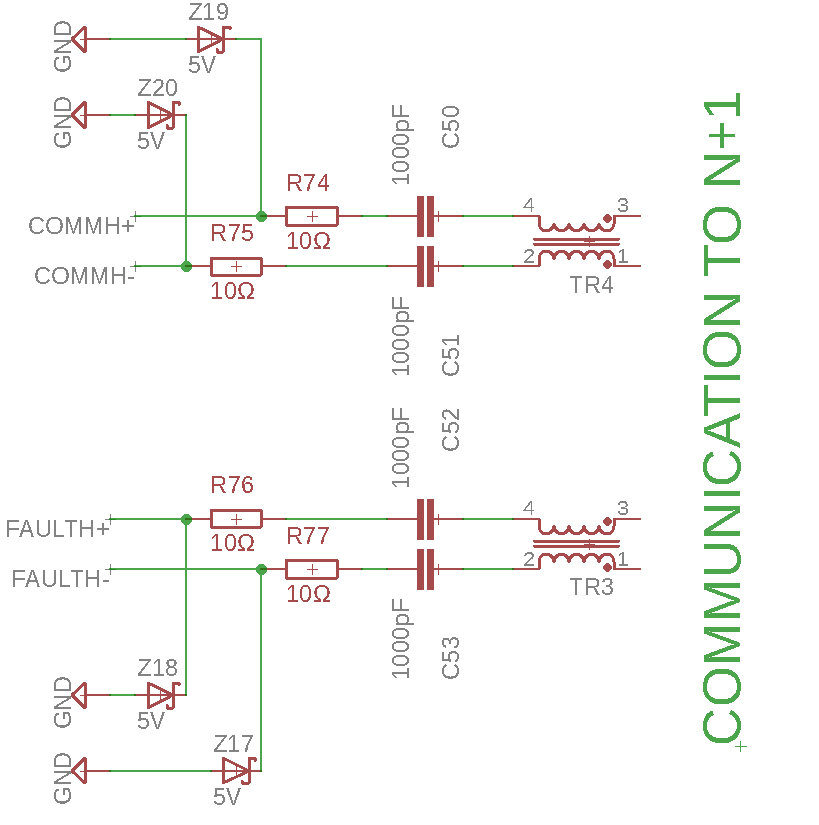
\includegraphics[width=\textwidth, height=12cm] {Prototip/schcomm+1.png}
    \caption{Comunicació amb el mòdul BQ76pl455a-q1 n+1.}
\end{figure}

\newpage

En canvi si estem parlant d'un mòdul esclau, aquest pot tenir els dos esquemàtics, és a dir, que ha de poder comunicar-se amb el mòdul inferior a ell i el mòdul superior a ell. Quan s'arriba a l'últim mòdul aquest només té l'esquemàtic per parlar amb el mòdul anterior. 

\begin{figure}[H]
	\centering
    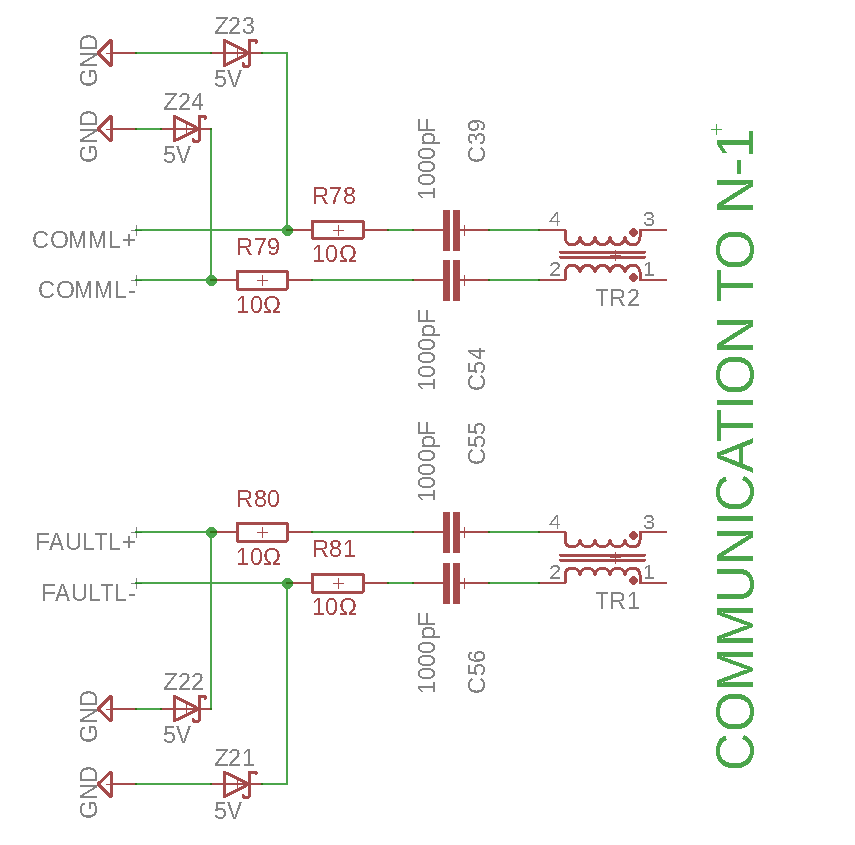
\includegraphics[width=\textwidth, height=14cm] {Prototip/schcomm-1.png}
    \caption{Comunicació amb el mòdul BQ76pl466a-q1 n-1.}
\end{figure}

\newpage 

La implementació d'ambdós esquemàtics és exactament la mateixa, amb la diferència de que estan connectats a diferents pins, ja que per comunicar-se amb el mòdul superior es parla a través dels pins acabats en H i per comunicar-se amb els inferiors amb els pins acabats en L. 

El circuit disposa de díodes zener, els quals limiten a que tot el voltatge sobrant no circuli pel circuit i sigui el zener qui l'atrapi. Amb això aconseguim que el voltatge no pugui sortir dels rangs de funcionament de les comunicacions. A més per comunicar entre dispositius BMS, el sistema de comunicacions queda totalment aïllat per un transformador (trafo). Aquest s'encarrega d'aïllar aquest voltatge per tal de poder-ho connectar de forma ideal al següent o anterior mòdul.

\subsection{Integrat BQ76pl455a-q1}

En aquest apartat tractarem l'integrat com a tal, encara que no es vegi d'una forma clara, s'utilitzen tots els pins d'aquest microcontrolador, \newline únicament que la connexió no es visible. El que si que es pot apreciar d'aquesta figura és com es realitza la comunicació entre la part que gestiona les bateries i la part que realitza el càlcul mitjançant els pins OUT. A més a més es veu la implementació dels pins CHP/CHM que s'utilitzen per a l'AFE. No s'ha entrat en detall en aquests aspectes degut a que simplement s'han seguit les especificacions del fabricant.

Cal destacar també que el VIO disposa de dos condensadors a massa per a evitar canvis bruscs de voltatge en aquest pin. 

\begin{figure}[H]
	\centering
    \includegraphics[width=\textwidth, height=15cm] {Prototip/schbq.png}
    \caption{Integrat BQ76pl455a-q1.}
\end{figure}

\newpage 

A més tampoc s'ha explicat res de les masses degut a que la implementació no ha pogut acabar de fer-se. El fabricant recomana l'utilització de diferents capes de massa a la PCB per tal d'evitar els retorns que els senyals analògics confronten amb els senyals digitals si van per la mateixa posició de la PCB. El fabricant mostra la següent figura indicant que cal realitzar aquesta diferenciació per tal de fer treballar el microcontrolador amb senyals el més nets possibles.

\begin{figure}[H]
	\centering
    \includegraphics[width=\textwidth, height=7cm] {Prototip/pcbgnd.png}
    \caption{Capa de masses de la futura PCB.}
\end{figure}

\newpage 

\subsection{Microcontrolador Atmel}
L'esquemàtic del microcontrolador ha estat extret del propi disseny de l'Arduino Mega. S'ha aprofitat tot el sector del rellotge del microcontrolador, del regulador de voltatge, per a què al micro li arribi un senyal pur de 5V i la implementació del reset. A més, per a poder carregar el programa al microcontrolador és precís d'un protocol de comunicacions entre un ordinador i aquest microcontrolador. La solució que normalment empra Arduino és mitjançant l'ús d'una comunicació Serial a partir de l'USB. El problema que té aquest tipus de comunicació és que requereix d'una electrònica molt més elaborada afegint un segon integrat (Atmega16U2), el qual permet gestionar el senyal provinent del Serial. És per això que la injecció de codi en el nostre cas es dóna a través del protocol SPI. L'integrat Atmega2560 permet el reconeixement d'aquest protocol de forma directa, amb la qual cosa només afegint un header per a poder connectar-nos nosaltres és suficient per a la injecció de codi.

El serial que s'utilitza per comunicar-nos entre el microcontrolador i el BQ és el Serial3, per el seu alt rendiment i configurabilitat. Els pins de GPIO es connecten al port A complert i els pins de WAKEUP i FAULTN es connecten als pins lliures del port B, que és el port més precís de l'Atmega2560.
\begin{figure}[H]
	\centering
    \includegraphics[width=\textwidth, height=10cm] {Prototip/schatmega2560.png}
    \caption{Implementació de l'Atmega 2560.}
\end{figure}
\chapter{Pressupost aproximat del prototip}
\label{chap:Pressupost del prototip}

%Introducció
Per falta de coneixements no s'ha pogut realitzar un prototip real funcional, el qual es pugui contrastar d'una forma objectiva i real amb \newline l'orionBMS, que era el que volíem mostrar. Tot i així si que podem fer una comparació a nivell econòmic per tal de veure per quin cost sortiria aquest BMS. S'han realitzat les recerques de components vàlids per a la implementació d'aquest prototip i s'han posat a més a més, els costos aproximats de la fabricació de la PCB i del muntatge mecànic i de soldadura de la PCB. Aquests preus de muntatge i fabricació estan contrastats amb els costos aproximats de l'empresa on hi treballo.

\begin{figure}[H]
	\centering
    \includegraphics[width=\textwidth, height=5cm] {Pressupost/costBMS.png}
\end{figure}

La llista de components queda mostrada a la següent taula:

\newpage

\begin{figure}[H]
	\centering
    \includegraphics[width=\textwidth, height=\textheight] {Pressupost/componentsp1.png}
\end{figure}

\begin{figure}[H]
	\centering
    \includegraphics[width=\textwidth, height=\textheight] {Pressupost/componentsp2.png}
\end{figure}
\chapter{Conclusions}
\label{chap:Conclusions}


Al llarg d'aquest projecte ens hem pogut adonar de tot l'abast que permet aquest camp de l'enginyeria. Hem pogut aprendre molts conceptes que ens serviran en el futur per a la nostra vida laboral. La tecnologia es va integrant en grans pasos a la societat i el món de les bateries i els vehicles elèctrics seran el futur sense cap mena de dubte. Amb aquests conceptes podem tenir una visió molt més crítica de la tecnologia en aquest camp. 

Actualment com hem vist amb el cas de l'OrionBMS els preus encara són molt cars, rondant els 1,000\$. Si la nostra alternativa de BMS s'arriba a implementar totalment, el preu de mercat podria arribar a competir amb el de l'OrionBMS i per tant, podem dir que la nostra idea de prototip s'apropa als models de gama alta del mercat. No obstant, les dificultats en la matèria han fet que només hàgim pogut arribar a implementar-ho a nivell esquemàtic. Falta una gran feina per a acabar tot el disseny i la part de software. Un cop dissenyat el BMS en la seva totalitat es podria implementar una interfície gràfica. Aquesta part ens resultaria molt més senzilla comparada amb el projecte, donat que és més el camp on ens hem format més. Un cop el producte estigués totalment implementat penso que seria un molt bon producte. 

Finalment cal dir que encara queda un llarg camí per a arribar a aconseguir el prototip de forma complerta. Encara que els preus estiguin molt per sota d'un BMS al mercat, la feina que encara queda per implementar-ho és lo suficientment gran com per no cantar victòria. Caldrà d'un gran esforç i futura dedicació per arribar a implementar aquest BMS a la vida real.


\begin{thebibliography}{X}
\bibitem{Baz} 
\textit{Bateries elèctriques}

https://es.wikipedia.org/wiki/Bateria\_electrica

http://www.areatecnologia.com/baterias-y-acumuladores.html

http://crashoil.blogspot.com/2014/06/apuntes-de-baterias-para-vehiculos.html

https://www.portatilmovil.com/blog/54\_carga-baterias-li-ion.html

http://elb105.com/battery-management-cargando-las-baterias/

\bibitem{asdf}
\textit{BMS}

http://www.intelite.com.mx/smart-hotels/conoces-como-funcionan-los-building-management-systems-bms/

https://www.youtube.com/watch?v=iSsDaH0SVzM

https://www.socomec.es/gama-almacenamiento-energia\_es.html?product=/flywheel\_es-1.html

https://www.orionbms.com/

https://cdn.shopify.com/s/files/1/1820/0269/files/\newline orion\_bms\_operational.pdf

https://foxbms.org/

http://docs.foxbms.org/en/latest/

http://bibing.us.es/proyectos/abreproy/5722/fichero/\newline Diseño+de+Sistemas+de+gestión+de+baterías.pdf

www.ti.com

\bibitem{VE}
\textit{Vehicles elèctrics}

www.amazon.es/

\bibitem{Prototipatge}
\textit{Prototipatge}

http://www.ti.com/product/BQ76PL455A-Q1

http://www.ti.com/lit/ds/symlink/bq76pl455a-q1.pdf

http://www.ti.com/lit/ds/symlink/bq76pl455a-q1.pdf

\end{thebibliography}


\bibliographystyle{apa}
\bibliography{thesis}


\end{document}